\documentclass[twoside]{book}

% Packages required by doxygen
\usepackage{fixltx2e}
\usepackage{calc}
\usepackage{doxygen}
\usepackage[export]{adjustbox} % also loads graphicx
\usepackage{graphicx}
\usepackage[utf8]{inputenc}
\usepackage{makeidx}
\usepackage{multicol}
\usepackage{multirow}
\PassOptionsToPackage{warn}{textcomp}
\usepackage{textcomp}
\usepackage[nointegrals]{wasysym}
\usepackage[table]{xcolor}

% NLS support packages
\usepackage[french]{babel}

% Font selection
\usepackage[T1]{fontenc}
\usepackage[scaled=.90]{helvet}
\usepackage{courier}
\usepackage{amssymb}
\usepackage{sectsty}
\renewcommand{\familydefault}{\sfdefault}
\allsectionsfont{%
  \fontseries{bc}\selectfont%
  \color{darkgray}%
}
\renewcommand{\DoxyLabelFont}{%
  \fontseries{bc}\selectfont%
  \color{darkgray}%
}
\newcommand{\+}{\discretionary{\mbox{\scriptsize$\hookleftarrow$}}{}{}}

% Page & text layout
\usepackage{geometry}
\geometry{%
  a4paper,%
  top=2.5cm,%
  bottom=2.5cm,%
  left=2.5cm,%
  right=2.5cm%
}
\tolerance=750
\hfuzz=15pt
\hbadness=750
\setlength{\emergencystretch}{15pt}
\setlength{\parindent}{0cm}
\setlength{\parskip}{3ex plus 2ex minus 2ex}
\makeatletter
\renewcommand{\paragraph}{%
  \@startsection{paragraph}{4}{0ex}{-1.0ex}{1.0ex}{%
    \normalfont\normalsize\bfseries\SS@parafont%
  }%
}
\renewcommand{\subparagraph}{%
  \@startsection{subparagraph}{5}{0ex}{-1.0ex}{1.0ex}{%
    \normalfont\normalsize\bfseries\SS@subparafont%
  }%
}
\makeatother

% Headers & footers
\usepackage{fancyhdr}
\pagestyle{fancyplain}
\fancyhead[LE]{\fancyplain{}{\bfseries\thepage}}
\fancyhead[CE]{\fancyplain{}{}}
\fancyhead[RE]{\fancyplain{}{\bfseries\leftmark}}
\fancyhead[LO]{\fancyplain{}{\bfseries\rightmark}}
\fancyhead[CO]{\fancyplain{}{}}
\fancyhead[RO]{\fancyplain{}{\bfseries\thepage}}
\fancyfoot[LE]{\fancyplain{}{}}
\fancyfoot[CE]{\fancyplain{}{}}
\fancyfoot[RE]{\fancyplain{}{\bfseries\scriptsize Généré par Doxygen }}
\fancyfoot[LO]{\fancyplain{}{\bfseries\scriptsize Généré par Doxygen }}
\fancyfoot[CO]{\fancyplain{}{}}
\fancyfoot[RO]{\fancyplain{}{}}
\renewcommand{\footrulewidth}{0.4pt}
\renewcommand{\chaptermark}[1]{%
  \markboth{#1}{}%
}
\renewcommand{\sectionmark}[1]{%
  \markright{\thesection\ #1}%
}

% Indices & bibliography
\usepackage{natbib}
\usepackage[titles]{tocloft}
\setcounter{tocdepth}{3}
\setcounter{secnumdepth}{5}
\makeindex

% Hyperlinks (required, but should be loaded last)
\usepackage{ifpdf}
\ifpdf
  \usepackage[pdftex,pagebackref=true]{hyperref}
\else
  \usepackage[ps2pdf,pagebackref=true]{hyperref}
\fi
\hypersetup{%
  colorlinks=true,%
  linkcolor=blue,%
  citecolor=blue,%
  unicode%
}

% Custom commands
\newcommand{\clearemptydoublepage}{%
  \newpage{\pagestyle{empty}\cleardoublepage}%
}

\usepackage{caption}
\captionsetup{labelsep=space,justification=centering,font={bf},singlelinecheck=off,skip=4pt,position=top}

%===== C O N T E N T S =====

\begin{document}

% Titlepage & ToC
\hypersetup{pageanchor=false,
             bookmarksnumbered=true,
             pdfencoding=unicode
            }
\pagenumbering{alph}
\begin{titlepage}
\vspace*{7cm}
\begin{center}%
{\Large Photobox }\\
\vspace*{1cm}
{\large Généré par Doxygen 1.8.13}\\
\end{center}
\end{titlepage}
\clearemptydoublepage
\pagenumbering{roman}
\tableofcontents
\clearemptydoublepage
\pagenumbering{arabic}
\hypersetup{pageanchor=true}

%--- Begin generated contents ---
\chapter{Index hiérarchique}
\section{Hiérarchie des classes}
Cette liste d\textquotesingle{}héritage est classée approximativement par ordre alphabétique \+:\begin{DoxyCompactList}
\item \contentsline{section}{Bibliotheque}{\pageref{classBibliotheque}}{}
\item \contentsline{section}{Image}{\pageref{classImage}}{}
\item Q\+Main\+Window\begin{DoxyCompactList}
\item \contentsline{section}{App\+Main\+Window}{\pageref{classAppMainWindow}}{}
\end{DoxyCompactList}
\end{DoxyCompactList}

\chapter{Index des classes}
\section{Liste des classes}
Liste des classes, structures, unions et interfaces avec une brève description \+:\begin{DoxyCompactList}
\item\contentsline{section}{\hyperlink{classAppMainWindow}{App\+Main\+Window} \\*The \hyperlink{classAppMainWindow}{App\+Main\+Window} class }{\pageref{classAppMainWindow}}{}
\item\contentsline{section}{\hyperlink{classBibliotheque}{Bibliotheque} \\*La classe \hyperlink{classBibliotheque}{Bibliotheque} permet la gestion d\textquotesingle{}une bibliotheque d\textquotesingle{}images }{\pageref{classBibliotheque}}{}
\item\contentsline{section}{\hyperlink{classImage}{Image} }{\pageref{classImage}}{}
\end{DoxyCompactList}

\chapter{Index des fichiers}
\section{Liste des fichiers}
Liste de tous les fichiers documentés avec une brève description \+:\begin{DoxyCompactList}
\item\contentsline{section}{\hyperlink{bibliotheque_8h}{bibliotheque.\+h} \\*Header de la classe \hyperlink{classBibliotheque}{Bibliotheque} }{\pageref{bibliotheque_8h}}{}
\item\contentsline{section}{{\bfseries complement.\+h} }{\pageref{complement_8h}}{}
\item\contentsline{section}{{\bfseries image.\+h} }{\pageref{image_8h}}{}
\item\contentsline{section}{{\bfseries mainwindow.\+h} }{\pageref{mainwindow_8h}}{}
\item\contentsline{section}{{\bfseries traitement\+Image.\+h} }{\pageref{traitementImage_8h}}{}
\end{DoxyCompactList}

\chapter{Documentation des classes}
\hypertarget{classBibliotheque}{}\section{Référence de la classe Bibliotheque}
\label{classBibliotheque}\index{Bibliotheque@{Bibliotheque}}


La classe \hyperlink{classBibliotheque}{Bibliotheque} permet la gestion d\textquotesingle{}une bibliotheque d\textquotesingle{}images.  




{\ttfamily \#include $<$bibliotheque.\+h$>$}

\subsection*{Fonctions membres publiques}
\begin{DoxyCompactItemize}
\item 
\mbox{\Hypertarget{classBibliotheque_a2b1ff298331a04c425926881e5f5ea49}\label{classBibliotheque_a2b1ff298331a04c425926881e5f5ea49}} 
\hyperlink{classBibliotheque_a2b1ff298331a04c425926881e5f5ea49}{Bibliotheque} ()
\begin{DoxyCompactList}\small\item\em Construire un nouveau objet \hyperlink{classBibliotheque}{Bibliotheque} vide. \end{DoxyCompactList}\item 
\hyperlink{classBibliotheque_ac18f721f99ed6699547099e554af08fe}{Bibliotheque} (string nom\+Bibliotheque)
\begin{DoxyCompactList}\small\item\em Construire un nouveau objet \hyperlink{classBibliotheque}{Bibliotheque} avec le nom de la bibliotheque. \end{DoxyCompactList}\item 
\hyperlink{classBibliotheque_abeef5fed51f37a993d77ba5af478051c}{Bibliotheque} (const Json\+::\+Value json\+Bibliotheque)
\begin{DoxyCompactList}\small\item\em Construire un nouveau objet \hyperlink{classBibliotheque}{Bibliotheque} avec un objet Json. \end{DoxyCompactList}\item 
Json\+::\+Value \hyperlink{classBibliotheque_a24b9cdc62d7bf2628e13ac9049dccaf3}{get\+Bilbiotheque} () const
\begin{DoxyCompactList}\small\item\em Obtenir l\textquotesingle{}objet Json de la \hyperlink{classBibliotheque}{Bibliotheque}. \end{DoxyCompactList}\item 
string \hyperlink{classBibliotheque_ace0c63ec27d7adfb7146406769f1a051}{get\+Chemin\+Json} () const
\begin{DoxyCompactList}\small\item\em Obtenir le chemin du fichier .json de la \hyperlink{classBibliotheque}{Bibliotheque}. \end{DoxyCompactList}\item 
void \hyperlink{classBibliotheque_a8dc396d28693e921f7fd849944356434}{set\+Bilbiotheque} (const Json\+::\+Value json\+Bibliotheque)
\begin{DoxyCompactList}\small\item\em Affecter l\textquotesingle{}objet Json de la Bilbiotheque. \end{DoxyCompactList}\item 
void \hyperlink{classBibliotheque_ac9201ed432b00fc3cd2621db1c8df78b}{set\+Chemin\+Json} (const string chemin\+Json)
\begin{DoxyCompactList}\small\item\em Affecter le chemin du fichier .json de la \hyperlink{classBibliotheque}{Bibliotheque}. \end{DoxyCompactList}\item 
void \hyperlink{classBibliotheque_a246e3a8893bb28b0d76845c624a1cd48}{Ajouter\+Image} (string chemin\+Acces\+Contenu, string titre, int numero, double cout, string source, string date\+Ajout, string date\+Creation, string acces)
\begin{DoxyCompactList}\small\item\em Ajouter une image a l\textquotesingle{}objet Json de la \hyperlink{classBibliotheque}{Bibliotheque}. \end{DoxyCompactList}\item 
void \hyperlink{classBibliotheque_a3e4940fd008650236beae91780d7b068}{Supprimer\+Image} (int numero)
\begin{DoxyCompactList}\small\item\em Supprimer une image de l\textquotesingle{}objet Json de la \hyperlink{classBibliotheque}{Bibliotheque}. \end{DoxyCompactList}\item 
void \hyperlink{classBibliotheque_abaf79da5c656d7cccb14b3c3a4b542f6}{Sauvegarder} (string file\+Name)
\begin{DoxyCompactList}\small\item\em Sauvegarder l\textquotesingle{}objet json de la \hyperlink{classBibliotheque}{Bibliotheque} dans un fichier .json. \end{DoxyCompactList}\item 
void \hyperlink{classBibliotheque_a61778c23eb938c95b4de4306c14fe754}{maj\+Biblio\+Suivant\+Droit\+Acces} (const bool droit\+Acces)
\begin{DoxyCompactList}\small\item\em Mettre à jour la \hyperlink{classBibliotheque}{Bibliotheque} suivant suivant les droits d\textquotesingle{}acces de l\textquotesingle{}utilisateur. ~\newline
 Si droit\+Acces = true (Utilisateur de Niveau 1) alors les images ayant un acces restreint sont supprimées de l\textquotesingle{}objet json de la \hyperlink{classBibliotheque}{Bibliotheque}. ~\newline
 Si droit\+Acces = false (Utilisateur de Niveau 2) alors on garde toutes les images dans l\textquotesingle{}objet json. \end{DoxyCompactList}\item 
Json\+::\+Value \hyperlink{classBibliotheque_a69655581e76d36176a4336a1504a2781}{Construire\+Afficher\+Sous\+Liste\+Cout} (const int choix)
\begin{DoxyCompactList}\small\item\em Construire une sous liste d\textquotesingle{}images de la \hyperlink{classBibliotheque}{Bibliotheque} suivant le choix de la plage de cout \+: ~\newline
 1 \+: gratuit ~\newline
 2 \+: cout $<$= 99,99€ ~\newline
 3 \+: cout $<$= 999,99€ ~\newline
 4 \+: cout $>$ 1000€ \end{DoxyCompactList}\item 
Json\+::\+Value \hyperlink{classBibliotheque_a3b03f7002bdb3bf8292ab5a676f74bf0}{Construire\+Afficher\+Sous\+Liste\+Cout} (double cout\+Min, double cout\+Max)
\begin{DoxyCompactList}\small\item\em Construire une sous liste d\textquotesingle{}images de la \hyperlink{classBibliotheque}{Bibliotheque} suivant la plage de cout \mbox{[}cout\+Min, cout\+Max\mbox{]}. \end{DoxyCompactList}\item 
Json\+::\+Value \hyperlink{classBibliotheque_a6b50b88a3f8f402052649e1bdc495b9a}{Construire\+Afficher\+Sous\+Liste\+Date\+Ajout} (const int choix)
\begin{DoxyCompactList}\small\item\em Construire une sous liste d\textquotesingle{}images de la \hyperlink{classBibliotheque}{Bibliotheque} suivant le choix de la plage de la date d\textquotesingle{}ajout \+: ~\newline
 1 \+: Ajouter aujourd\textquotesingle{}hui ~\newline
 2 \+: Ajouter il y a moins de 7 jours ~\newline
 3 \+: Ajouter ce mois ~\newline
 4 \+: Ajouter cette annee. \end{DoxyCompactList}\item 
Json\+::\+Value \hyperlink{classBibliotheque_aa06803a5d680126cdbddbe4e1ab9395c}{Trier} (const int choix)
\begin{DoxyCompactList}\small\item\em Trier l\textquotesingle{}objet json de la \hyperlink{classBibliotheque}{Bibliotheque} suivant les critères \+: ~\newline
 1 \+: Cout decroissant ~\newline
 2 \+: Numero decroissant ~\newline
 3 \+: Acces Restreint puis Acces Publique. \end{DoxyCompactList}\item 
vector$<$ int $>$ \hyperlink{classBibliotheque_ad62c3fc7fd3829a0634a22ad98aa9332}{Trier} (vector$<$ double $>$ valeur\+Non\+Tri)
\begin{DoxyCompactList}\small\item\em Trier un vecteur de reels dans l\textquotesingle{}ordre décroissant. \end{DoxyCompactList}\item 
vector$<$ int $>$ \hyperlink{classBibliotheque_af95534b5f7fba8f1a6dcd1215bd55f96}{Trier} (vector$<$ string $>$ valeur\+Non\+Tri)
\begin{DoxyCompactList}\small\item\em Trier un vecteur de chaines characteres dans l\textquotesingle{}ordre décroissant. \end{DoxyCompactList}\item 
vector$<$ int $>$ \hyperlink{classBibliotheque_a0a0c1d628bfa840f764d4ec483f4b1e6}{Trier} (vector$<$ int $>$ valeur\+Non\+Tri)
\begin{DoxyCompactList}\small\item\em Trier un vecteur d\textquotesingle{}entiers dans l\textquotesingle{}ordre décroissant. \end{DoxyCompactList}\end{DoxyCompactItemize}
\subsection*{Attributs privés}
\begin{DoxyCompactItemize}
\item 
\mbox{\Hypertarget{classBibliotheque_a15a693b9eedd442d0cc00489b5ea6e5e}\label{classBibliotheque_a15a693b9eedd442d0cc00489b5ea6e5e}} 
Json\+::\+Value \hyperlink{classBibliotheque_a15a693b9eedd442d0cc00489b5ea6e5e}{\+\_\+bibliotheque}
\begin{DoxyCompactList}\small\item\em Objet Json de la bibliotheque. \end{DoxyCompactList}\item 
\mbox{\Hypertarget{classBibliotheque_a9628b7dc59bbb3894c17634addc8016a}\label{classBibliotheque_a9628b7dc59bbb3894c17634addc8016a}} 
string \hyperlink{classBibliotheque_a9628b7dc59bbb3894c17634addc8016a}{\+\_\+chemin\+Json}
\begin{DoxyCompactList}\small\item\em Chemin du fichier .json de la bibliotheque. \end{DoxyCompactList}\end{DoxyCompactItemize}


\subsection{Description détaillée}
La classe \hyperlink{classBibliotheque}{Bibliotheque} permet la gestion d\textquotesingle{}une bibliotheque d\textquotesingle{}images. 

\subsection{Documentation des constructeurs et destructeur}
\mbox{\Hypertarget{classBibliotheque_ac18f721f99ed6699547099e554af08fe}\label{classBibliotheque_ac18f721f99ed6699547099e554af08fe}} 
\index{Bibliotheque@{Bibliotheque}!Bibliotheque@{Bibliotheque}}
\index{Bibliotheque@{Bibliotheque}!Bibliotheque@{Bibliotheque}}
\subsubsection{\texorpdfstring{Bibliotheque()}{Bibliotheque()}\hspace{0.1cm}{\footnotesize\ttfamily [1/2]}}
{\footnotesize\ttfamily Bibliotheque\+::\+Bibliotheque (\begin{DoxyParamCaption}\item[{string}]{nom\+Bibliotheque }\end{DoxyParamCaption})}



Construire un nouveau objet \hyperlink{classBibliotheque}{Bibliotheque} avec le nom de la bibliotheque. 


\begin{DoxyParams}{Paramètres}
{\em nom\+Bibliotheque} & string \\
\hline
\end{DoxyParams}
\mbox{\Hypertarget{classBibliotheque_abeef5fed51f37a993d77ba5af478051c}\label{classBibliotheque_abeef5fed51f37a993d77ba5af478051c}} 
\index{Bibliotheque@{Bibliotheque}!Bibliotheque@{Bibliotheque}}
\index{Bibliotheque@{Bibliotheque}!Bibliotheque@{Bibliotheque}}
\subsubsection{\texorpdfstring{Bibliotheque()}{Bibliotheque()}\hspace{0.1cm}{\footnotesize\ttfamily [2/2]}}
{\footnotesize\ttfamily Bibliotheque\+::\+Bibliotheque (\begin{DoxyParamCaption}\item[{const Json\+::\+Value}]{json\+Bibliotheque }\end{DoxyParamCaption})}



Construire un nouveau objet \hyperlink{classBibliotheque}{Bibliotheque} avec un objet Json. 


\begin{DoxyParams}{Paramètres}
{\em json\+Bibliotheque} & Json\+::\+Value \\
\hline
\end{DoxyParams}


\subsection{Documentation des fonctions membres}
\mbox{\Hypertarget{classBibliotheque_a246e3a8893bb28b0d76845c624a1cd48}\label{classBibliotheque_a246e3a8893bb28b0d76845c624a1cd48}} 
\index{Bibliotheque@{Bibliotheque}!Ajouter\+Image@{Ajouter\+Image}}
\index{Ajouter\+Image@{Ajouter\+Image}!Bibliotheque@{Bibliotheque}}
\subsubsection{\texorpdfstring{Ajouter\+Image()}{AjouterImage()}}
{\footnotesize\ttfamily void Bibliotheque\+::\+Ajouter\+Image (\begin{DoxyParamCaption}\item[{string}]{chemin\+Acces\+Contenu,  }\item[{string}]{titre,  }\item[{int}]{numero,  }\item[{double}]{cout,  }\item[{string}]{source,  }\item[{string}]{date\+Ajout,  }\item[{string}]{date\+Creation,  }\item[{string}]{acces }\end{DoxyParamCaption})}



Ajouter une image a l\textquotesingle{}objet Json de la \hyperlink{classBibliotheque}{Bibliotheque}. 


\begin{DoxyParams}{Paramètres}
{\em chemin\+Acces\+Contenu} & string \\
\hline
{\em titre} & string \\
\hline
{\em numero} & int \\
\hline
{\em cout} & double \\
\hline
{\em source} & string \\
\hline
{\em date\+Ajout} & string \\
\hline
{\em date\+Creation} & string \\
\hline
{\em acces} & string \\
\hline
\end{DoxyParams}
\mbox{\Hypertarget{classBibliotheque_a69655581e76d36176a4336a1504a2781}\label{classBibliotheque_a69655581e76d36176a4336a1504a2781}} 
\index{Bibliotheque@{Bibliotheque}!Construire\+Afficher\+Sous\+Liste\+Cout@{Construire\+Afficher\+Sous\+Liste\+Cout}}
\index{Construire\+Afficher\+Sous\+Liste\+Cout@{Construire\+Afficher\+Sous\+Liste\+Cout}!Bibliotheque@{Bibliotheque}}
\subsubsection{\texorpdfstring{Construire\+Afficher\+Sous\+Liste\+Cout()}{ConstruireAfficherSousListeCout()}\hspace{0.1cm}{\footnotesize\ttfamily [1/2]}}
{\footnotesize\ttfamily Json\+::\+Value Bibliotheque\+::\+Construire\+Afficher\+Sous\+Liste\+Cout (\begin{DoxyParamCaption}\item[{const int}]{choix }\end{DoxyParamCaption})}



Construire une sous liste d\textquotesingle{}images de la \hyperlink{classBibliotheque}{Bibliotheque} suivant le choix de la plage de cout \+: ~\newline
 1 \+: gratuit ~\newline
 2 \+: cout $<$= 99,99€ ~\newline
 3 \+: cout $<$= 999,99€ ~\newline
 4 \+: cout $>$ 1000€ 


\begin{DoxyParams}{Paramètres}
{\em choix} & int \\
\hline
\end{DoxyParams}
\begin{DoxyReturn}{Renvoie}
Json\+::\+Value \+: un objet json contenant la sous liste construite. 
\end{DoxyReturn}
\mbox{\Hypertarget{classBibliotheque_a3b03f7002bdb3bf8292ab5a676f74bf0}\label{classBibliotheque_a3b03f7002bdb3bf8292ab5a676f74bf0}} 
\index{Bibliotheque@{Bibliotheque}!Construire\+Afficher\+Sous\+Liste\+Cout@{Construire\+Afficher\+Sous\+Liste\+Cout}}
\index{Construire\+Afficher\+Sous\+Liste\+Cout@{Construire\+Afficher\+Sous\+Liste\+Cout}!Bibliotheque@{Bibliotheque}}
\subsubsection{\texorpdfstring{Construire\+Afficher\+Sous\+Liste\+Cout()}{ConstruireAfficherSousListeCout()}\hspace{0.1cm}{\footnotesize\ttfamily [2/2]}}
{\footnotesize\ttfamily Json\+::\+Value Bibliotheque\+::\+Construire\+Afficher\+Sous\+Liste\+Cout (\begin{DoxyParamCaption}\item[{double}]{cout\+Min,  }\item[{double}]{cout\+Max }\end{DoxyParamCaption})}



Construire une sous liste d\textquotesingle{}images de la \hyperlink{classBibliotheque}{Bibliotheque} suivant la plage de cout \mbox{[}cout\+Min, cout\+Max\mbox{]}. 


\begin{DoxyParams}{Paramètres}
{\em cout\+Min} & double \\
\hline
{\em cout\+Max} & double \\
\hline
\end{DoxyParams}
\begin{DoxyReturn}{Renvoie}
Json\+::\+Value \+: un objet json contenant la sous liste construite. 
\end{DoxyReturn}
\mbox{\Hypertarget{classBibliotheque_a6b50b88a3f8f402052649e1bdc495b9a}\label{classBibliotheque_a6b50b88a3f8f402052649e1bdc495b9a}} 
\index{Bibliotheque@{Bibliotheque}!Construire\+Afficher\+Sous\+Liste\+Date\+Ajout@{Construire\+Afficher\+Sous\+Liste\+Date\+Ajout}}
\index{Construire\+Afficher\+Sous\+Liste\+Date\+Ajout@{Construire\+Afficher\+Sous\+Liste\+Date\+Ajout}!Bibliotheque@{Bibliotheque}}
\subsubsection{\texorpdfstring{Construire\+Afficher\+Sous\+Liste\+Date\+Ajout()}{ConstruireAfficherSousListeDateAjout()}}
{\footnotesize\ttfamily Json\+::\+Value Bibliotheque\+::\+Construire\+Afficher\+Sous\+Liste\+Date\+Ajout (\begin{DoxyParamCaption}\item[{const int}]{choix }\end{DoxyParamCaption})}



Construire une sous liste d\textquotesingle{}images de la \hyperlink{classBibliotheque}{Bibliotheque} suivant le choix de la plage de la date d\textquotesingle{}ajout \+: ~\newline
 1 \+: Ajouter aujourd\textquotesingle{}hui ~\newline
 2 \+: Ajouter il y a moins de 7 jours ~\newline
 3 \+: Ajouter ce mois ~\newline
 4 \+: Ajouter cette annee. 


\begin{DoxyParams}{Paramètres}
{\em choix} & int \\
\hline
\end{DoxyParams}
\begin{DoxyReturn}{Renvoie}
Json\+::\+Value \+: un objet json contenant la sous liste construite suivant le critère choisi. 
\end{DoxyReturn}
\mbox{\Hypertarget{classBibliotheque_a24b9cdc62d7bf2628e13ac9049dccaf3}\label{classBibliotheque_a24b9cdc62d7bf2628e13ac9049dccaf3}} 
\index{Bibliotheque@{Bibliotheque}!get\+Bilbiotheque@{get\+Bilbiotheque}}
\index{get\+Bilbiotheque@{get\+Bilbiotheque}!Bibliotheque@{Bibliotheque}}
\subsubsection{\texorpdfstring{get\+Bilbiotheque()}{getBilbiotheque()}}
{\footnotesize\ttfamily Json\+::\+Value Bibliotheque\+::get\+Bilbiotheque (\begin{DoxyParamCaption}{ }\end{DoxyParamCaption}) const}



Obtenir l\textquotesingle{}objet Json de la \hyperlink{classBibliotheque}{Bibliotheque}. 

\begin{DoxyReturn}{Renvoie}
Json\+::\+Value \+: l\textquotesingle{}objet Json de la \hyperlink{classBibliotheque}{Bibliotheque} 
\end{DoxyReturn}
\mbox{\Hypertarget{classBibliotheque_ace0c63ec27d7adfb7146406769f1a051}\label{classBibliotheque_ace0c63ec27d7adfb7146406769f1a051}} 
\index{Bibliotheque@{Bibliotheque}!get\+Chemin\+Json@{get\+Chemin\+Json}}
\index{get\+Chemin\+Json@{get\+Chemin\+Json}!Bibliotheque@{Bibliotheque}}
\subsubsection{\texorpdfstring{get\+Chemin\+Json()}{getCheminJson()}}
{\footnotesize\ttfamily string Bibliotheque\+::get\+Chemin\+Json (\begin{DoxyParamCaption}{ }\end{DoxyParamCaption}) const}



Obtenir le chemin du fichier .json de la \hyperlink{classBibliotheque}{Bibliotheque}. 

\begin{DoxyReturn}{Renvoie}
string \+: une chaine de charactere contenant le chemin du fichier .json de la \hyperlink{classBibliotheque}{Bibliotheque}. 
\end{DoxyReturn}
\mbox{\Hypertarget{classBibliotheque_a61778c23eb938c95b4de4306c14fe754}\label{classBibliotheque_a61778c23eb938c95b4de4306c14fe754}} 
\index{Bibliotheque@{Bibliotheque}!maj\+Biblio\+Suivant\+Droit\+Acces@{maj\+Biblio\+Suivant\+Droit\+Acces}}
\index{maj\+Biblio\+Suivant\+Droit\+Acces@{maj\+Biblio\+Suivant\+Droit\+Acces}!Bibliotheque@{Bibliotheque}}
\subsubsection{\texorpdfstring{maj\+Biblio\+Suivant\+Droit\+Acces()}{majBiblioSuivantDroitAcces()}}
{\footnotesize\ttfamily void Bibliotheque\+::maj\+Biblio\+Suivant\+Droit\+Acces (\begin{DoxyParamCaption}\item[{const bool}]{droit\+Acces }\end{DoxyParamCaption})}



Mettre à jour la \hyperlink{classBibliotheque}{Bibliotheque} suivant suivant les droits d\textquotesingle{}acces de l\textquotesingle{}utilisateur. ~\newline
 Si droit\+Acces = true (Utilisateur de Niveau 1) alors les images ayant un acces restreint sont supprimées de l\textquotesingle{}objet json de la \hyperlink{classBibliotheque}{Bibliotheque}. ~\newline
 Si droit\+Acces = false (Utilisateur de Niveau 2) alors on garde toutes les images dans l\textquotesingle{}objet json. 


\begin{DoxyParams}{Paramètres}
{\em droit\+Acces} & bool \\
\hline
\end{DoxyParams}
\mbox{\Hypertarget{classBibliotheque_abaf79da5c656d7cccb14b3c3a4b542f6}\label{classBibliotheque_abaf79da5c656d7cccb14b3c3a4b542f6}} 
\index{Bibliotheque@{Bibliotheque}!Sauvegarder@{Sauvegarder}}
\index{Sauvegarder@{Sauvegarder}!Bibliotheque@{Bibliotheque}}
\subsubsection{\texorpdfstring{Sauvegarder()}{Sauvegarder()}}
{\footnotesize\ttfamily void Bibliotheque\+::\+Sauvegarder (\begin{DoxyParamCaption}\item[{string}]{file\+Name }\end{DoxyParamCaption})}



Sauvegarder l\textquotesingle{}objet json de la \hyperlink{classBibliotheque}{Bibliotheque} dans un fichier .json. 


\begin{DoxyParams}{Paramètres}
{\em file\+Name} & string \\
\hline
\end{DoxyParams}
\mbox{\Hypertarget{classBibliotheque_a8dc396d28693e921f7fd849944356434}\label{classBibliotheque_a8dc396d28693e921f7fd849944356434}} 
\index{Bibliotheque@{Bibliotheque}!set\+Bilbiotheque@{set\+Bilbiotheque}}
\index{set\+Bilbiotheque@{set\+Bilbiotheque}!Bibliotheque@{Bibliotheque}}
\subsubsection{\texorpdfstring{set\+Bilbiotheque()}{setBilbiotheque()}}
{\footnotesize\ttfamily void Bibliotheque\+::set\+Bilbiotheque (\begin{DoxyParamCaption}\item[{const Json\+::\+Value}]{json\+Bibliotheque }\end{DoxyParamCaption})}



Affecter l\textquotesingle{}objet Json de la Bilbiotheque. 


\begin{DoxyParams}{Paramètres}
{\em json\+Bibliotheque} & Json\+::\+Value \\
\hline
\end{DoxyParams}
\mbox{\Hypertarget{classBibliotheque_ac9201ed432b00fc3cd2621db1c8df78b}\label{classBibliotheque_ac9201ed432b00fc3cd2621db1c8df78b}} 
\index{Bibliotheque@{Bibliotheque}!set\+Chemin\+Json@{set\+Chemin\+Json}}
\index{set\+Chemin\+Json@{set\+Chemin\+Json}!Bibliotheque@{Bibliotheque}}
\subsubsection{\texorpdfstring{set\+Chemin\+Json()}{setCheminJson()}}
{\footnotesize\ttfamily void Bibliotheque\+::set\+Chemin\+Json (\begin{DoxyParamCaption}\item[{const string}]{chemin\+Json }\end{DoxyParamCaption})}



Affecter le chemin du fichier .json de la \hyperlink{classBibliotheque}{Bibliotheque}. 


\begin{DoxyParams}{Paramètres}
{\em chemin\+Json} & string \\
\hline
\end{DoxyParams}
\mbox{\Hypertarget{classBibliotheque_a3e4940fd008650236beae91780d7b068}\label{classBibliotheque_a3e4940fd008650236beae91780d7b068}} 
\index{Bibliotheque@{Bibliotheque}!Supprimer\+Image@{Supprimer\+Image}}
\index{Supprimer\+Image@{Supprimer\+Image}!Bibliotheque@{Bibliotheque}}
\subsubsection{\texorpdfstring{Supprimer\+Image()}{SupprimerImage()}}
{\footnotesize\ttfamily void Bibliotheque\+::\+Supprimer\+Image (\begin{DoxyParamCaption}\item[{int}]{numero }\end{DoxyParamCaption})}



Supprimer une image de l\textquotesingle{}objet Json de la \hyperlink{classBibliotheque}{Bibliotheque}. 


\begin{DoxyParams}{Paramètres}
{\em numero} & int \\
\hline
\end{DoxyParams}
\mbox{\Hypertarget{classBibliotheque_aa06803a5d680126cdbddbe4e1ab9395c}\label{classBibliotheque_aa06803a5d680126cdbddbe4e1ab9395c}} 
\index{Bibliotheque@{Bibliotheque}!Trier@{Trier}}
\index{Trier@{Trier}!Bibliotheque@{Bibliotheque}}
\subsubsection{\texorpdfstring{Trier()}{Trier()}\hspace{0.1cm}{\footnotesize\ttfamily [1/4]}}
{\footnotesize\ttfamily Json\+::\+Value Bibliotheque\+::\+Trier (\begin{DoxyParamCaption}\item[{const int}]{choix }\end{DoxyParamCaption})}



Trier l\textquotesingle{}objet json de la \hyperlink{classBibliotheque}{Bibliotheque} suivant les critères \+: ~\newline
 1 \+: Cout decroissant ~\newline
 2 \+: Numero decroissant ~\newline
 3 \+: Acces Restreint puis Acces Publique. 


\begin{DoxyParams}{Paramètres}
{\em choix} & \\
\hline
\end{DoxyParams}
\begin{DoxyReturn}{Renvoie}
Json\+::\+Value \+: un objet json de contenant une bibliothèque triée suivant le critère choisi. 
\end{DoxyReturn}
\mbox{\Hypertarget{classBibliotheque_ad62c3fc7fd3829a0634a22ad98aa9332}\label{classBibliotheque_ad62c3fc7fd3829a0634a22ad98aa9332}} 
\index{Bibliotheque@{Bibliotheque}!Trier@{Trier}}
\index{Trier@{Trier}!Bibliotheque@{Bibliotheque}}
\subsubsection{\texorpdfstring{Trier()}{Trier()}\hspace{0.1cm}{\footnotesize\ttfamily [2/4]}}
{\footnotesize\ttfamily vector$<$int$>$ Bibliotheque\+::\+Trier (\begin{DoxyParamCaption}\item[{vector$<$ double $>$}]{valeur\+Non\+Tri }\end{DoxyParamCaption})}



Trier un vecteur de reels dans l\textquotesingle{}ordre décroissant. 


\begin{DoxyParams}{Paramètres}
{\em valeur\+Non\+Tri} & vector$<$double$>$ \\
\hline
\end{DoxyParams}
\begin{DoxyReturn}{Renvoie}
vector$<$int$>$ \+: un vecteur d\textquotesingle{}entiers contenant les indices triés du vecteur d\textquotesingle{}entrée. 
\end{DoxyReturn}
\mbox{\Hypertarget{classBibliotheque_af95534b5f7fba8f1a6dcd1215bd55f96}\label{classBibliotheque_af95534b5f7fba8f1a6dcd1215bd55f96}} 
\index{Bibliotheque@{Bibliotheque}!Trier@{Trier}}
\index{Trier@{Trier}!Bibliotheque@{Bibliotheque}}
\subsubsection{\texorpdfstring{Trier()}{Trier()}\hspace{0.1cm}{\footnotesize\ttfamily [3/4]}}
{\footnotesize\ttfamily vector$<$int$>$ Bibliotheque\+::\+Trier (\begin{DoxyParamCaption}\item[{vector$<$ string $>$}]{valeur\+Non\+Tri }\end{DoxyParamCaption})}



Trier un vecteur de chaines characteres dans l\textquotesingle{}ordre décroissant. 


\begin{DoxyParams}{Paramètres}
{\em valeur\+Non\+Tri} & vector$<$string$>$ \\
\hline
\end{DoxyParams}
\begin{DoxyReturn}{Renvoie}
vector$<$int$>$ \+: un vecteur d\textquotesingle{}entiers contenant les indices triés du vecteur d\textquotesingle{}entrée. 
\end{DoxyReturn}
\mbox{\Hypertarget{classBibliotheque_a0a0c1d628bfa840f764d4ec483f4b1e6}\label{classBibliotheque_a0a0c1d628bfa840f764d4ec483f4b1e6}} 
\index{Bibliotheque@{Bibliotheque}!Trier@{Trier}}
\index{Trier@{Trier}!Bibliotheque@{Bibliotheque}}
\subsubsection{\texorpdfstring{Trier()}{Trier()}\hspace{0.1cm}{\footnotesize\ttfamily [4/4]}}
{\footnotesize\ttfamily vector$<$int$>$ Bibliotheque\+::\+Trier (\begin{DoxyParamCaption}\item[{vector$<$ int $>$}]{valeur\+Non\+Tri }\end{DoxyParamCaption})}



Trier un vecteur d\textquotesingle{}entiers dans l\textquotesingle{}ordre décroissant. 


\begin{DoxyParams}{Paramètres}
{\em valeur\+Non\+Tri} & vector$<$int$>$ \\
\hline
\end{DoxyParams}
\begin{DoxyReturn}{Renvoie}
vector$<$int$>$ \+: un vecteur d\textquotesingle{}entiers contenant les indices triés du vecteur d\textquotesingle{}entrée. 
\end{DoxyReturn}


La documentation de cette classe a été générée à partir du fichier suivant \+:\begin{DoxyCompactItemize}
\item 
\hyperlink{bibliotheque_8h}{bibliotheque.\+h}\end{DoxyCompactItemize}

\hypertarget{classMainWindow}{}\section{Référence de la classe Main\+Window}
\label{classMainWindow}\index{Main\+Window@{Main\+Window}}


The \hyperlink{classMainWindow}{Main\+Window} class.  




{\ttfamily \#include $<$mainwindow.\+h$>$}



Graphe d\textquotesingle{}héritage de Main\+Window\+:
\nopagebreak
\begin{figure}[H]
\begin{center}
\leavevmode
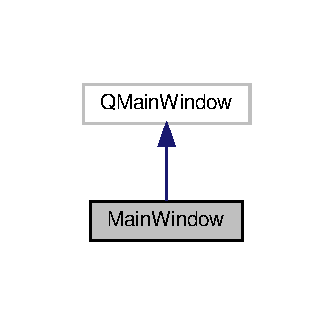
\includegraphics[width=160pt]{classMainWindow__inherit__graph}
\end{center}
\end{figure}


Graphe de collaboration de Main\+Window\+:
\nopagebreak
\begin{figure}[H]
\begin{center}
\leavevmode
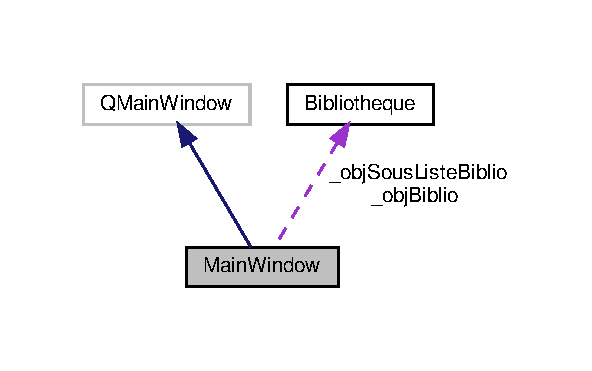
\includegraphics[width=284pt]{classMainWindow__coll__graph}
\end{center}
\end{figure}
\subsection*{Fonctions membres publiques}
\begin{DoxyCompactItemize}
\item 
\mbox{\Hypertarget{classMainWindow_a8b244be8b7b7db1b08de2a2acb9409db}\label{classMainWindow_a8b244be8b7b7db1b08de2a2acb9409db}} 
{\bfseries Main\+Window} (Q\+Widget $\ast$parent=0)
\end{DoxyCompactItemize}
\subsection*{Connecteurs privés}
\begin{DoxyCompactItemize}
\item 
\mbox{\Hypertarget{classMainWindow_a288eee5287611da2b2e5844478e7c928}\label{classMainWindow_a288eee5287611da2b2e5844478e7c928}} 
void \hyperlink{classMainWindow_a288eee5287611da2b2e5844478e7c928}{on\+\_\+push\+Button\+Identifier\+\_\+clicked} ()
\begin{DoxyCompactList}\small\item\em on\+\_\+push\+Button\+Identifier\+\_\+clicked \end{DoxyCompactList}\item 
\mbox{\Hypertarget{classMainWindow_a94045fe84db5691c70d2bb3e806f0812}\label{classMainWindow_a94045fe84db5691c70d2bb3e806f0812}} 
void \hyperlink{classMainWindow_a94045fe84db5691c70d2bb3e806f0812}{on\+\_\+push\+Button\+Quitter\+\_\+clicked} ()
\begin{DoxyCompactList}\small\item\em on\+\_\+push\+Button\+Quitter\+\_\+clicked \end{DoxyCompactList}\item 
\mbox{\Hypertarget{classMainWindow_a46c11c6c090ccb3cd8f9584c2b9dbf48}\label{classMainWindow_a46c11c6c090ccb3cd8f9584c2b9dbf48}} 
void \hyperlink{classMainWindow_a46c11c6c090ccb3cd8f9584c2b9dbf48}{on\+\_\+push\+Button\+Charger\+Biblio\+\_\+clicked} ()
\begin{DoxyCompactList}\small\item\em on\+\_\+push\+Button\+Charger\+Biblio\+\_\+clicked \end{DoxyCompactList}\item 
\mbox{\Hypertarget{classMainWindow_a141877383fb575d9e847e22ac7d274c7}\label{classMainWindow_a141877383fb575d9e847e22ac7d274c7}} 
void \hyperlink{classMainWindow_a141877383fb575d9e847e22ac7d274c7}{on\+\_\+push\+Button\+Retour\+Identification\+\_\+clicked} ()
\begin{DoxyCompactList}\small\item\em on\+\_\+push\+Button\+Retour\+Identification\+\_\+clicked \end{DoxyCompactList}\item 
\mbox{\Hypertarget{classMainWindow_a97069de59e1201e639a2dc064e6d2427}\label{classMainWindow_a97069de59e1201e639a2dc064e6d2427}} 
void \hyperlink{classMainWindow_a97069de59e1201e639a2dc064e6d2427}{on\+\_\+table\+Biblio\+Row\+Clicked} (int, int)
\begin{DoxyCompactList}\small\item\em on\+\_\+table\+Biblio\+Row\+Clicked \end{DoxyCompactList}\item 
\mbox{\Hypertarget{classMainWindow_a93279e87f7a6aa808619892c0c5f2f4a}\label{classMainWindow_a93279e87f7a6aa808619892c0c5f2f4a}} 
void \hyperlink{classMainWindow_a93279e87f7a6aa808619892c0c5f2f4a}{on\+\_\+push\+Button\+Sauvegarder\+\_\+clicked} ()
\begin{DoxyCompactList}\small\item\em on\+\_\+push\+Button\+Sauvegarder\+\_\+clicked \end{DoxyCompactList}\item 
\mbox{\Hypertarget{classMainWindow_ab4183704bae96b91f47d6f186612d4f9}\label{classMainWindow_ab4183704bae96b91f47d6f186612d4f9}} 
void \hyperlink{classMainWindow_ab4183704bae96b91f47d6f186612d4f9}{on\+\_\+push\+Button\+Supprimer\+Image\+\_\+clicked} ()
\begin{DoxyCompactList}\small\item\em on\+\_\+push\+Button\+Supprimer\+Image\+\_\+clicked \end{DoxyCompactList}\item 
\mbox{\Hypertarget{classMainWindow_a2ec76fe0831835fa115ccfca42297af6}\label{classMainWindow_a2ec76fe0831835fa115ccfca42297af6}} 
void \hyperlink{classMainWindow_a2ec76fe0831835fa115ccfca42297af6}{on\+\_\+push\+Button\+Retour\+Menu\+Principal\+\_\+clicked} ()
\begin{DoxyCompactList}\small\item\em on\+\_\+push\+Button\+Retour\+Menu\+Principal\+\_\+clicked \end{DoxyCompactList}\item 
\mbox{\Hypertarget{classMainWindow_a495b1763c99152a0a067d9efcd5867b6}\label{classMainWindow_a495b1763c99152a0a067d9efcd5867b6}} 
void \hyperlink{classMainWindow_a495b1763c99152a0a067d9efcd5867b6}{on\+\_\+line\+Edit\+Mdp\+\_\+return\+Pressed} ()
\begin{DoxyCompactList}\small\item\em on\+\_\+line\+Edit\+Mdp\+\_\+return\+Pressed \end{DoxyCompactList}\item 
\mbox{\Hypertarget{classMainWindow_ab6cdf8f1b4ab60072dc0ba1940e3544d}\label{classMainWindow_ab6cdf8f1b4ab60072dc0ba1940e3544d}} 
void \hyperlink{classMainWindow_ab6cdf8f1b4ab60072dc0ba1940e3544d}{on\+\_\+combo\+Box\+Trier\+Index\+Changed} (int)
\begin{DoxyCompactList}\small\item\em on\+\_\+combo\+Box\+Trier\+Index\+Changed \end{DoxyCompactList}\item 
\mbox{\Hypertarget{classMainWindow_a4ce966ee5dac14ecc0d7faf13fbe974d}\label{classMainWindow_a4ce966ee5dac14ecc0d7faf13fbe974d}} 
void \hyperlink{classMainWindow_a4ce966ee5dac14ecc0d7faf13fbe974d}{on\+\_\+combo\+Box\+Critere\+Cout\+Index\+Changed} (int)
\begin{DoxyCompactList}\small\item\em on\+\_\+combo\+Box\+Critere\+Cout\+Index\+Changed \end{DoxyCompactList}\item 
\mbox{\Hypertarget{classMainWindow_afd34abf465e165a2d8e3aa3b65451ee9}\label{classMainWindow_afd34abf465e165a2d8e3aa3b65451ee9}} 
void \hyperlink{classMainWindow_afd34abf465e165a2d8e3aa3b65451ee9}{on\+\_\+combo\+Box\+Critere\+Date\+Ajout\+Index\+Changed} (int)
\begin{DoxyCompactList}\small\item\em on\+\_\+combo\+Box\+Critere\+Date\+Ajout\+Index\+Changed \end{DoxyCompactList}\item 
\mbox{\Hypertarget{classMainWindow_a16d6f34d51ccffec28fc667cce4c4800}\label{classMainWindow_a16d6f34d51ccffec28fc667cce4c4800}} 
void \hyperlink{classMainWindow_a16d6f34d51ccffec28fc667cce4c4800}{on\+\_\+push\+Button\+Ajouter\+Image\+\_\+clicked} ()
\begin{DoxyCompactList}\small\item\em on\+\_\+push\+Button\+Ajouter\+Image\+\_\+clicked \end{DoxyCompactList}\item 
\mbox{\Hypertarget{classMainWindow_af8e692c3bce912dbdaf87e66db8ed9bc}\label{classMainWindow_af8e692c3bce912dbdaf87e66db8ed9bc}} 
void \hyperlink{classMainWindow_af8e692c3bce912dbdaf87e66db8ed9bc}{on\+\_\+push\+Button\+Ajout\+Image\+Annuler\+\_\+clicked} ()
\begin{DoxyCompactList}\small\item\em on\+\_\+push\+Button\+Ajout\+Image\+Annuler\+\_\+clicked \end{DoxyCompactList}\item 
\mbox{\Hypertarget{classMainWindow_a99a0007db57453254e82797b4eb4bf1a}\label{classMainWindow_a99a0007db57453254e82797b4eb4bf1a}} 
void \hyperlink{classMainWindow_a99a0007db57453254e82797b4eb4bf1a}{on\+\_\+push\+Button\+Ajout\+Image\+Ajouter\+\_\+clicked} ()
\begin{DoxyCompactList}\small\item\em on\+\_\+push\+Button\+Ajout\+Image\+Ajouter\+\_\+clicked \end{DoxyCompactList}\item 
\mbox{\Hypertarget{classMainWindow_ac70efc539a8c362a65469329f58e0db1}\label{classMainWindow_ac70efc539a8c362a65469329f58e0db1}} 
void \hyperlink{classMainWindow_ac70efc539a8c362a65469329f58e0db1}{on\+\_\+push\+Button\+Creer\+Biblio\+\_\+clicked} ()
\begin{DoxyCompactList}\small\item\em on\+\_\+push\+Button\+Creer\+Biblio\+\_\+clicked \end{DoxyCompactList}\item 
\mbox{\Hypertarget{classMainWindow_a9e4fb81b32de37afdbbddfa67288452a}\label{classMainWindow_a9e4fb81b32de37afdbbddfa67288452a}} 
void \hyperlink{classMainWindow_a9e4fb81b32de37afdbbddfa67288452a}{on\+\_\+push\+Button\+Sauvegarder\+Sous\+Liste\+\_\+clicked} ()
\begin{DoxyCompactList}\small\item\em on\+\_\+push\+Button\+Sauvegarder\+Sous\+Liste\+\_\+clicked \end{DoxyCompactList}\item 
\mbox{\Hypertarget{classMainWindow_a07a876cbbff67e47d60cbda1316d5b75}\label{classMainWindow_a07a876cbbff67e47d60cbda1316d5b75}} 
void \hyperlink{classMainWindow_a07a876cbbff67e47d60cbda1316d5b75}{on\+\_\+push\+Button\+Ouvrir\+Image\+\_\+clicked} ()
\begin{DoxyCompactList}\small\item\em on\+\_\+push\+Button\+Ouvrir\+Image\+\_\+clicked \end{DoxyCompactList}\item 
\mbox{\Hypertarget{classMainWindow_ae1ca6c5420cf50c889056f3732b271bf}\label{classMainWindow_ae1ca6c5420cf50c889056f3732b271bf}} 
void \hyperlink{classMainWindow_ae1ca6c5420cf50c889056f3732b271bf}{on\+\_\+push\+Button\+Retour\+Menu\+Modification\+Image\+\_\+clicked} ()
\begin{DoxyCompactList}\small\item\em on\+\_\+push\+Button\+Retour\+Menu\+Modification\+Image\+\_\+clicked \end{DoxyCompactList}\item 
\mbox{\Hypertarget{classMainWindow_a94b88633fa3b8b6eb9727f973f20a8a1}\label{classMainWindow_a94b88633fa3b8b6eb9727f973f20a8a1}} 
void \hyperlink{classMainWindow_a94b88633fa3b8b6eb9727f973f20a8a1}{on\+\_\+double\+Spin\+Box\+Min\+\_\+value\+Changed} (double)
\begin{DoxyCompactList}\small\item\em on\+\_\+double\+Spin\+Box\+Min\+\_\+value\+Changed \end{DoxyCompactList}\item 
\mbox{\Hypertarget{classMainWindow_a9c2d4a213092fef9a1ca6341bf01f558}\label{classMainWindow_a9c2d4a213092fef9a1ca6341bf01f558}} 
void \hyperlink{classMainWindow_a9c2d4a213092fef9a1ca6341bf01f558}{on\+\_\+double\+Spin\+Box\+Max\+\_\+value\+Changed} (double)
\begin{DoxyCompactList}\small\item\em on\+\_\+double\+Spin\+Box\+Max\+\_\+value\+Changed \end{DoxyCompactList}\item 
\mbox{\Hypertarget{classMainWindow_a37fc7ed847837660646dcf4d315f72b6}\label{classMainWindow_a37fc7ed847837660646dcf4d315f72b6}} 
void \hyperlink{classMainWindow_a37fc7ed847837660646dcf4d315f72b6}{on\+\_\+horizontal\+Slider\+\_\+agrandissement\+Non\+Modifiable\+\_\+value\+Changed} (int)
\begin{DoxyCompactList}\small\item\em on\+\_\+horizontal\+Slider\+\_\+agrandissement\+Non\+Modifiable\+\_\+value\+Changed \end{DoxyCompactList}\item 
\mbox{\Hypertarget{classMainWindow_a70f495382f691edf5ac4c5b754249c21}\label{classMainWindow_a70f495382f691edf5ac4c5b754249c21}} 
void \hyperlink{classMainWindow_a70f495382f691edf5ac4c5b754249c21}{on\+\_\+push\+Button\+\_\+modifier\+\_\+clicked} ()
\begin{DoxyCompactList}\small\item\em on\+\_\+push\+Button\+\_\+modifier\+\_\+clicked \end{DoxyCompactList}\item 
\mbox{\Hypertarget{classMainWindow_acb133bc5aa31c34985de1f1d29ad17f9}\label{classMainWindow_acb133bc5aa31c34985de1f1d29ad17f9}} 
void \hyperlink{classMainWindow_acb133bc5aa31c34985de1f1d29ad17f9}{on\+\_\+horizontal\+Slider\+\_\+agrandissement\+\_\+value\+Changed} (int)
\begin{DoxyCompactList}\small\item\em on\+\_\+horizontal\+Slider\+\_\+agrandissement\+\_\+value\+Changed \end{DoxyCompactList}\item 
\mbox{\Hypertarget{classMainWindow_adf60caef775208cb39eff294981c9e88}\label{classMainWindow_adf60caef775208cb39eff294981c9e88}} 
void \hyperlink{classMainWindow_adf60caef775208cb39eff294981c9e88}{on\+\_\+push\+Button\+\_\+traitement\+Image\+\_\+clicked} ()
\begin{DoxyCompactList}\small\item\em on\+\_\+push\+Button\+\_\+traitement\+Image\+\_\+clicked \end{DoxyCompactList}\item 
\mbox{\Hypertarget{classMainWindow_aec65250d1c32225746ec18aa394a943f}\label{classMainWindow_aec65250d1c32225746ec18aa394a943f}} 
void \hyperlink{classMainWindow_aec65250d1c32225746ec18aa394a943f}{on\+\_\+push\+Button\+\_\+retour\+\_\+clicked} ()
\begin{DoxyCompactList}\small\item\em on\+\_\+push\+Button\+\_\+retour\+\_\+clicked \end{DoxyCompactList}\item 
\mbox{\Hypertarget{classMainWindow_aa9835b27970c4d853eda5430f168145f}\label{classMainWindow_aa9835b27970c4d853eda5430f168145f}} 
void \hyperlink{classMainWindow_aa9835b27970c4d853eda5430f168145f}{on\+\_\+horizontal\+Slider\+\_\+image\+Originale\+\_\+value\+Changed} (int)
\begin{DoxyCompactList}\small\item\em on\+\_\+horizontal\+Slider\+\_\+image\+Originale\+\_\+value\+Changed \end{DoxyCompactList}\item 
\mbox{\Hypertarget{classMainWindow_aa02bacdc44ef7bf15d0ed596a08c30a7}\label{classMainWindow_aa02bacdc44ef7bf15d0ed596a08c30a7}} 
void \hyperlink{classMainWindow_aa02bacdc44ef7bf15d0ed596a08c30a7}{on\+\_\+horizontal\+Slider\+\_\+image\+Traitee\+\_\+value\+Changed} (int)
\begin{DoxyCompactList}\small\item\em on\+\_\+horizontal\+Slider\+\_\+image\+Traitee\+\_\+value\+Changed \end{DoxyCompactList}\item 
\mbox{\Hypertarget{classMainWindow_a13a2050ed2e2434b34f8e78917782680}\label{classMainWindow_a13a2050ed2e2434b34f8e78917782680}} 
void \hyperlink{classMainWindow_a13a2050ed2e2434b34f8e78917782680}{on\+\_\+push\+Button\+\_\+traitement\+Reinitialiser\+\_\+clicked} ()
\begin{DoxyCompactList}\small\item\em on\+\_\+push\+Button\+\_\+traitement\+Reinitialiser\+\_\+clicked \end{DoxyCompactList}\item 
\mbox{\Hypertarget{classMainWindow_a95dfac4432df7db5a514e297568d9c4b}\label{classMainWindow_a95dfac4432df7db5a514e297568d9c4b}} 
void \hyperlink{classMainWindow_a95dfac4432df7db5a514e297568d9c4b}{on\+\_\+push\+Button\+\_\+traitement\+Appliquer\+\_\+clicked} ()
\begin{DoxyCompactList}\small\item\em on\+\_\+push\+Button\+\_\+traitement\+Appliquer\+\_\+clicked \end{DoxyCompactList}\item 
\mbox{\Hypertarget{classMainWindow_af6a18794abeab4023d0c80e287c7f27c}\label{classMainWindow_af6a18794abeab4023d0c80e287c7f27c}} 
void \hyperlink{classMainWindow_af6a18794abeab4023d0c80e287c7f27c}{on\+\_\+group\+Box\+\_\+correction\+\_\+clicked} ()
\begin{DoxyCompactList}\small\item\em on\+\_\+group\+Box\+\_\+correction\+\_\+clicked \end{DoxyCompactList}\item 
\mbox{\Hypertarget{classMainWindow_a46cfe3aff7aa1b223f0b34aaf251e351}\label{classMainWindow_a46cfe3aff7aa1b223f0b34aaf251e351}} 
void \hyperlink{classMainWindow_a46cfe3aff7aa1b223f0b34aaf251e351}{on\+\_\+radio\+Button\+\_\+luminosite\+\_\+clicked} ()
\begin{DoxyCompactList}\small\item\em on\+\_\+radio\+Button\+\_\+luminosite\+\_\+clicked \end{DoxyCompactList}\item 
\mbox{\Hypertarget{classMainWindow_a049310c5a29f1b9b0a948e08865ac470}\label{classMainWindow_a049310c5a29f1b9b0a948e08865ac470}} 
void \hyperlink{classMainWindow_a049310c5a29f1b9b0a948e08865ac470}{on\+\_\+horizontal\+Slider\+\_\+luminosite\+\_\+value\+Changed} (int)
\begin{DoxyCompactList}\small\item\em on\+\_\+horizontal\+Slider\+\_\+luminosite\+\_\+value\+Changed \end{DoxyCompactList}\item 
\mbox{\Hypertarget{classMainWindow_ad38ae230bebcd4dc68b5a2fe5c18cf4b}\label{classMainWindow_ad38ae230bebcd4dc68b5a2fe5c18cf4b}} 
void \hyperlink{classMainWindow_ad38ae230bebcd4dc68b5a2fe5c18cf4b}{on\+\_\+radio\+Button\+\_\+contraste\+\_\+clicked} ()
\begin{DoxyCompactList}\small\item\em on\+\_\+radio\+Button\+\_\+contraste\+\_\+clicked \end{DoxyCompactList}\item 
\mbox{\Hypertarget{classMainWindow_adb1efa488197404fc8e27cd0864348bd}\label{classMainWindow_adb1efa488197404fc8e27cd0864348bd}} 
void \hyperlink{classMainWindow_adb1efa488197404fc8e27cd0864348bd}{on\+\_\+horizontal\+Slider\+\_\+contraste\+\_\+value\+Changed} (int)
\begin{DoxyCompactList}\small\item\em on\+\_\+horizontal\+Slider\+\_\+contraste\+\_\+value\+Changed \end{DoxyCompactList}\item 
\mbox{\Hypertarget{classMainWindow_ab70e3fe99b0d5341caf390b77a7f139b}\label{classMainWindow_ab70e3fe99b0d5341caf390b77a7f139b}} 
void \hyperlink{classMainWindow_ab70e3fe99b0d5341caf390b77a7f139b}{on\+\_\+radio\+Button\+\_\+ombre\+\_\+clicked} ()
\begin{DoxyCompactList}\small\item\em on\+\_\+radio\+Button\+\_\+ombre\+\_\+clicked \end{DoxyCompactList}\item 
\mbox{\Hypertarget{classMainWindow_ac0eee404a887a264d0c7b7f5e2fd5c16}\label{classMainWindow_ac0eee404a887a264d0c7b7f5e2fd5c16}} 
void \hyperlink{classMainWindow_ac0eee404a887a264d0c7b7f5e2fd5c16}{on\+\_\+horizontal\+Slider\+\_\+ombre\+\_\+value\+Changed} (int)
\begin{DoxyCompactList}\small\item\em on\+\_\+horizontal\+Slider\+\_\+ombre\+\_\+value\+Changed \end{DoxyCompactList}\item 
\mbox{\Hypertarget{classMainWindow_ad4ac905771cedf7d802d6ce7b0fa242e}\label{classMainWindow_ad4ac905771cedf7d802d6ce7b0fa242e}} 
void \hyperlink{classMainWindow_ad4ac905771cedf7d802d6ce7b0fa242e}{on\+\_\+radio\+Button\+\_\+brillance\+\_\+clicked} ()
\begin{DoxyCompactList}\small\item\em on\+\_\+radio\+Button\+\_\+brillance\+\_\+clicked \end{DoxyCompactList}\item 
\mbox{\Hypertarget{classMainWindow_a2f09785d376668bf1df5508753e3a66d}\label{classMainWindow_a2f09785d376668bf1df5508753e3a66d}} 
void \hyperlink{classMainWindow_a2f09785d376668bf1df5508753e3a66d}{on\+\_\+horizontal\+Slider\+\_\+brillance\+\_\+value\+Changed} (int)
\begin{DoxyCompactList}\small\item\em on\+\_\+horizontal\+Slider\+\_\+brillance\+\_\+value\+Changed \end{DoxyCompactList}\item 
\mbox{\Hypertarget{classMainWindow_a38b3e512cfc669706a4238dc17aa8d1f}\label{classMainWindow_a38b3e512cfc669706a4238dc17aa8d1f}} 
void \hyperlink{classMainWindow_a38b3e512cfc669706a4238dc17aa8d1f}{on\+\_\+group\+Box\+\_\+details\+\_\+clicked} ()
\begin{DoxyCompactList}\small\item\em on\+\_\+group\+Box\+\_\+details\+\_\+clicked \end{DoxyCompactList}\item 
\mbox{\Hypertarget{classMainWindow_a2f78b38c6a3ea4b7d0515b4f10dc2c0e}\label{classMainWindow_a2f78b38c6a3ea4b7d0515b4f10dc2c0e}} 
void \hyperlink{classMainWindow_a2f78b38c6a3ea4b7d0515b4f10dc2c0e}{on\+\_\+radio\+Button\+\_\+nettete\+\_\+clicked} ()
\begin{DoxyCompactList}\small\item\em on\+\_\+radio\+Button\+\_\+nettete\+\_\+clicked \end{DoxyCompactList}\item 
\mbox{\Hypertarget{classMainWindow_a3db26b38033cbb9eb6ff08f6aa50abcb}\label{classMainWindow_a3db26b38033cbb9eb6ff08f6aa50abcb}} 
void \hyperlink{classMainWindow_a3db26b38033cbb9eb6ff08f6aa50abcb}{on\+\_\+horizontal\+Slider\+\_\+nettete\+\_\+value\+Changed} (int)
\begin{DoxyCompactList}\small\item\em on\+\_\+horizontal\+Slider\+\_\+nettete\+\_\+value\+Changed \end{DoxyCompactList}\item 
\mbox{\Hypertarget{classMainWindow_a9b6edbac08ead702bbfcd04d6b416831}\label{classMainWindow_a9b6edbac08ead702bbfcd04d6b416831}} 
void \hyperlink{classMainWindow_a9b6edbac08ead702bbfcd04d6b416831}{on\+\_\+radio\+Button\+\_\+bruitage\+\_\+clicked} ()
\begin{DoxyCompactList}\small\item\em on\+\_\+radio\+Button\+\_\+bruitage\+\_\+clicked \end{DoxyCompactList}\item 
\mbox{\Hypertarget{classMainWindow_a9b8d63047bfc67fb655e6a98a1231984}\label{classMainWindow_a9b8d63047bfc67fb655e6a98a1231984}} 
void \hyperlink{classMainWindow_a9b8d63047bfc67fb655e6a98a1231984}{on\+\_\+horizontal\+Slider\+\_\+\+Bruitage\+\_\+value\+Changed} (int)
\begin{DoxyCompactList}\small\item\em on\+\_\+horizontal\+Slider\+\_\+\+Bruitage\+\_\+value\+Changed \end{DoxyCompactList}\item 
\mbox{\Hypertarget{classMainWindow_a5358808e6910fab1d30a8a5215e29ae7}\label{classMainWindow_a5358808e6910fab1d30a8a5215e29ae7}} 
void \hyperlink{classMainWindow_a5358808e6910fab1d30a8a5215e29ae7}{on\+\_\+group\+Box\+\_\+filtres\+\_\+clicked} ()
\begin{DoxyCompactList}\small\item\em on\+\_\+group\+Box\+\_\+filtres\+\_\+clicked \end{DoxyCompactList}\item 
\mbox{\Hypertarget{classMainWindow_ad8f6a3b5cb5accbb03bf20a0aa7c8e49}\label{classMainWindow_ad8f6a3b5cb5accbb03bf20a0aa7c8e49}} 
void \hyperlink{classMainWindow_ad8f6a3b5cb5accbb03bf20a0aa7c8e49}{on\+\_\+radio\+Button\+\_\+originale\+\_\+clicked} ()
\begin{DoxyCompactList}\small\item\em on\+\_\+radio\+Button\+\_\+originale\+\_\+clicked \end{DoxyCompactList}\item 
\mbox{\Hypertarget{classMainWindow_a9eb58116f007312b8b77c997308a2290}\label{classMainWindow_a9eb58116f007312b8b77c997308a2290}} 
void \hyperlink{classMainWindow_a9eb58116f007312b8b77c997308a2290}{on\+\_\+radio\+Button\+\_\+niveau\+Gris\+\_\+clicked} ()
\begin{DoxyCompactList}\small\item\em on\+\_\+radio\+Button\+\_\+niveau\+Gris\+\_\+clicked \end{DoxyCompactList}\item 
\mbox{\Hypertarget{classMainWindow_a8a4f1cd0f33bc30dc04761c2f7267f20}\label{classMainWindow_a8a4f1cd0f33bc30dc04761c2f7267f20}} 
void \hyperlink{classMainWindow_a8a4f1cd0f33bc30dc04761c2f7267f20}{on\+\_\+radio\+Button\+\_\+inversement\+\_\+clicked} ()
\begin{DoxyCompactList}\small\item\em on\+\_\+radio\+Button\+\_\+inversement\+\_\+clicked \end{DoxyCompactList}\item 
\mbox{\Hypertarget{classMainWindow_a9d571dd0b7fc606e4881e237a720d295}\label{classMainWindow_a9d571dd0b7fc606e4881e237a720d295}} 
void \hyperlink{classMainWindow_a9d571dd0b7fc606e4881e237a720d295}{on\+\_\+radio\+Button\+\_\+rouge\+\_\+clicked} ()
\begin{DoxyCompactList}\small\item\em on\+\_\+radio\+Button\+\_\+rouge\+\_\+clicked \end{DoxyCompactList}\item 
\mbox{\Hypertarget{classMainWindow_a7e733a84b4d9544190ce8f4a85a42b5f}\label{classMainWindow_a7e733a84b4d9544190ce8f4a85a42b5f}} 
void \hyperlink{classMainWindow_a7e733a84b4d9544190ce8f4a85a42b5f}{on\+\_\+radio\+Button\+\_\+vert\+\_\+clicked} ()
\begin{DoxyCompactList}\small\item\em on\+\_\+radio\+Button\+\_\+vert\+\_\+clicked \end{DoxyCompactList}\item 
\mbox{\Hypertarget{classMainWindow_a6b57e90800526b9218644e5569b40471}\label{classMainWindow_a6b57e90800526b9218644e5569b40471}} 
void \hyperlink{classMainWindow_a6b57e90800526b9218644e5569b40471}{on\+\_\+radio\+Button\+\_\+bleu\+\_\+clicked} ()
\begin{DoxyCompactList}\small\item\em on\+\_\+radio\+Button\+\_\+bleu\+\_\+clicked \end{DoxyCompactList}\item 
\mbox{\Hypertarget{classMainWindow_ae618d92ac47808e6f846fde6f7549277}\label{classMainWindow_ae618d92ac47808e6f846fde6f7549277}} 
void \hyperlink{classMainWindow_ae618d92ac47808e6f846fde6f7549277}{on\+\_\+radio\+Button\+\_\+jaune\+\_\+clicked} ()
\begin{DoxyCompactList}\small\item\em on\+\_\+radio\+Button\+\_\+jaune\+\_\+clicked \end{DoxyCompactList}\item 
\mbox{\Hypertarget{classMainWindow_a4ce0e94016a53d79e6cdf6eaf8b7a417}\label{classMainWindow_a4ce0e94016a53d79e6cdf6eaf8b7a417}} 
void \hyperlink{classMainWindow_a4ce0e94016a53d79e6cdf6eaf8b7a417}{on\+\_\+radio\+Button\+\_\+cyan\+\_\+clicked} ()
\begin{DoxyCompactList}\small\item\em on\+\_\+radio\+Button\+\_\+cyan\+\_\+clicked \end{DoxyCompactList}\item 
\mbox{\Hypertarget{classMainWindow_a330ba7333408e84f5259c55bab38a033}\label{classMainWindow_a330ba7333408e84f5259c55bab38a033}} 
void \hyperlink{classMainWindow_a330ba7333408e84f5259c55bab38a033}{on\+\_\+radio\+Button\+\_\+sepia\+\_\+clicked} ()
\begin{DoxyCompactList}\small\item\em on\+\_\+radio\+Button\+\_\+sepia\+\_\+clicked \end{DoxyCompactList}\item 
\mbox{\Hypertarget{classMainWindow_ad90a23f641924d6cf4c5f399bdb22c2e}\label{classMainWindow_ad90a23f641924d6cf4c5f399bdb22c2e}} 
void \hyperlink{classMainWindow_ad90a23f641924d6cf4c5f399bdb22c2e}{on\+\_\+radio\+Button\+\_\+magenta\+\_\+clicked} ()
\begin{DoxyCompactList}\small\item\em on\+\_\+radio\+Button\+\_\+magenta\+\_\+clicked \end{DoxyCompactList}\item 
\mbox{\Hypertarget{classMainWindow_a029c841c8d1452bab969569f3001840a}\label{classMainWindow_a029c841c8d1452bab969569f3001840a}} 
void \hyperlink{classMainWindow_a029c841c8d1452bab969569f3001840a}{on\+\_\+radio\+Button\+\_\+rgb\+\_\+clicked} ()
\begin{DoxyCompactList}\small\item\em on\+\_\+radio\+Button\+\_\+rgb\+\_\+clicked \end{DoxyCompactList}\item 
\mbox{\Hypertarget{classMainWindow_a643b2edab2f78bab60c3e3dd5993409e}\label{classMainWindow_a643b2edab2f78bab60c3e3dd5993409e}} 
void \hyperlink{classMainWindow_a643b2edab2f78bab60c3e3dd5993409e}{on\+\_\+group\+Box\+\_\+extraction\+R\+V\+B\+\_\+clicked} ()
\begin{DoxyCompactList}\small\item\em on\+\_\+group\+Box\+\_\+extraction\+R\+V\+B\+\_\+clicked \end{DoxyCompactList}\item 
\mbox{\Hypertarget{classMainWindow_a70993f7b7d5f3cbd67979813234da83a}\label{classMainWindow_a70993f7b7d5f3cbd67979813234da83a}} 
void \hyperlink{classMainWindow_a70993f7b7d5f3cbd67979813234da83a}{on\+\_\+radio\+Button\+\_\+extraction\+R\+\_\+clicked} ()
\begin{DoxyCompactList}\small\item\em on\+\_\+radio\+Button\+\_\+extraction\+R\+\_\+clicked \end{DoxyCompactList}\item 
\mbox{\Hypertarget{classMainWindow_a73f419590c6daf7f3a40fe480c22779a}\label{classMainWindow_a73f419590c6daf7f3a40fe480c22779a}} 
void \hyperlink{classMainWindow_a73f419590c6daf7f3a40fe480c22779a}{on\+\_\+radio\+Button\+\_\+extraction\+V\+\_\+clicked} ()
\begin{DoxyCompactList}\small\item\em on\+\_\+radio\+Button\+\_\+extraction\+V\+\_\+clicked \end{DoxyCompactList}\item 
\mbox{\Hypertarget{classMainWindow_a1632f39c370309f84beef1262e176cc0}\label{classMainWindow_a1632f39c370309f84beef1262e176cc0}} 
void \hyperlink{classMainWindow_a1632f39c370309f84beef1262e176cc0}{on\+\_\+radio\+Button\+\_\+extraction\+B\+\_\+clicked} ()
\begin{DoxyCompactList}\small\item\em on\+\_\+radio\+Button\+\_\+extraction\+B\+\_\+clicked \end{DoxyCompactList}\item 
\mbox{\Hypertarget{classMainWindow_a550c0d329f7ddaef00162e5960e75d3d}\label{classMainWindow_a550c0d329f7ddaef00162e5960e75d3d}} 
void \hyperlink{classMainWindow_a550c0d329f7ddaef00162e5960e75d3d}{on\+\_\+group\+Box\+\_\+seuillage\+Segmentation\+\_\+clicked} ()
\begin{DoxyCompactList}\small\item\em on\+\_\+group\+Box\+\_\+seuillage\+Segmentation\+\_\+clicked \end{DoxyCompactList}\item 
\mbox{\Hypertarget{classMainWindow_a2674db4d7c9dca3608d7bba7e5c19712}\label{classMainWindow_a2674db4d7c9dca3608d7bba7e5c19712}} 
void \hyperlink{classMainWindow_a2674db4d7c9dca3608d7bba7e5c19712}{on\+\_\+radio\+Button\+\_\+seuillage\+\_\+clicked} ()
\begin{DoxyCompactList}\small\item\em on\+\_\+radio\+Button\+\_\+seuillage\+\_\+clicked \end{DoxyCompactList}\item 
\mbox{\Hypertarget{classMainWindow_abcf9df73bb70a451ebec8981b9de97a5}\label{classMainWindow_abcf9df73bb70a451ebec8981b9de97a5}} 
void \hyperlink{classMainWindow_abcf9df73bb70a451ebec8981b9de97a5}{on\+\_\+radio\+Button\+\_\+segmentation\+\_\+clicked} ()
\begin{DoxyCompactList}\small\item\em on\+\_\+radio\+Button\+\_\+segmentation\+\_\+clicked \end{DoxyCompactList}\item 
\mbox{\Hypertarget{classMainWindow_acd3de1b1aba25842b7cd46f6b16a7e14}\label{classMainWindow_acd3de1b1aba25842b7cd46f6b16a7e14}} 
void \hyperlink{classMainWindow_acd3de1b1aba25842b7cd46f6b16a7e14}{on\+\_\+radio\+Button\+\_\+seuillage\+Simple\+\_\+clicked} ()
\begin{DoxyCompactList}\small\item\em on\+\_\+radio\+Button\+\_\+seuillage\+Simple\+\_\+clicked \end{DoxyCompactList}\item 
\mbox{\Hypertarget{classMainWindow_a86a77b82762aa811b0a89cc8be7ce59e}\label{classMainWindow_a86a77b82762aa811b0a89cc8be7ce59e}} 
void \hyperlink{classMainWindow_a86a77b82762aa811b0a89cc8be7ce59e}{on\+\_\+radio\+Button\+\_\+seuillage\+Hysteresis\+\_\+clicked} ()
\begin{DoxyCompactList}\small\item\em on\+\_\+radio\+Button\+\_\+seuillage\+Hysteresis\+\_\+clicked \end{DoxyCompactList}\item 
\mbox{\Hypertarget{classMainWindow_a8d42f39e072db3ba34dbd693fb3e03b1}\label{classMainWindow_a8d42f39e072db3ba34dbd693fb3e03b1}} 
void \hyperlink{classMainWindow_a8d42f39e072db3ba34dbd693fb3e03b1}{on\+\_\+vertical\+Slider\+\_\+seuil\+Bas\+R\+\_\+2\+\_\+value\+Changed} (int)
\begin{DoxyCompactList}\small\item\em on\+\_\+vertical\+Slider\+\_\+seuil\+Bas\+R\+\_\+2\+\_\+value\+Changed \end{DoxyCompactList}\item 
\mbox{\Hypertarget{classMainWindow_aff55460fade4cfec35d634a75e53f2b0}\label{classMainWindow_aff55460fade4cfec35d634a75e53f2b0}} 
void \hyperlink{classMainWindow_aff55460fade4cfec35d634a75e53f2b0}{on\+\_\+vertical\+Slider\+\_\+seuil\+Bas\+V\+\_\+2\+\_\+value\+Changed} (int)
\begin{DoxyCompactList}\small\item\em on\+\_\+vertical\+Slider\+\_\+seuil\+Bas\+V\+\_\+2\+\_\+value\+Changed \end{DoxyCompactList}\item 
\mbox{\Hypertarget{classMainWindow_a4da5b6fd53c17717eb29e287a0d3b49d}\label{classMainWindow_a4da5b6fd53c17717eb29e287a0d3b49d}} 
void \hyperlink{classMainWindow_a4da5b6fd53c17717eb29e287a0d3b49d}{on\+\_\+vertical\+Slider\+\_\+seuil\+Bas\+B\+\_\+2\+\_\+value\+Changed} (int)
\begin{DoxyCompactList}\small\item\em on\+\_\+vertical\+Slider\+\_\+seuil\+Bas\+B\+\_\+2\+\_\+value\+Changed \end{DoxyCompactList}\item 
\mbox{\Hypertarget{classMainWindow_adb86796f8b99a463f50b10cd98d44676}\label{classMainWindow_adb86796f8b99a463f50b10cd98d44676}} 
void \hyperlink{classMainWindow_adb86796f8b99a463f50b10cd98d44676}{on\+\_\+vertical\+Slider\+\_\+seuil\+Haut\+R\+\_\+2\+\_\+value\+Changed} (int)
\begin{DoxyCompactList}\small\item\em on\+\_\+vertical\+Slider\+\_\+seuil\+Haut\+R\+\_\+2\+\_\+value\+Changed \end{DoxyCompactList}\item 
\mbox{\Hypertarget{classMainWindow_a7800e4bb1bbfe1e956e4379ce7127677}\label{classMainWindow_a7800e4bb1bbfe1e956e4379ce7127677}} 
void \hyperlink{classMainWindow_a7800e4bb1bbfe1e956e4379ce7127677}{on\+\_\+vertical\+Slider\+\_\+seuil\+Haut\+V\+\_\+2\+\_\+value\+Changed} (int)
\begin{DoxyCompactList}\small\item\em on\+\_\+vertical\+Slider\+\_\+seuil\+Haut\+V\+\_\+2\+\_\+value\+Changed \end{DoxyCompactList}\item 
\mbox{\Hypertarget{classMainWindow_a697625302189c63431547221bc6cbab2}\label{classMainWindow_a697625302189c63431547221bc6cbab2}} 
void \hyperlink{classMainWindow_a697625302189c63431547221bc6cbab2}{on\+\_\+vertical\+Slider\+\_\+seuil\+Haut\+B\+\_\+2\+\_\+value\+Changed} (int)
\begin{DoxyCompactList}\small\item\em on\+\_\+vertical\+Slider\+\_\+seuil\+Haut\+B\+\_\+2\+\_\+value\+Changed \end{DoxyCompactList}\item 
\mbox{\Hypertarget{classMainWindow_a5818966b3d0af54935e5bd1675c94665}\label{classMainWindow_a5818966b3d0af54935e5bd1675c94665}} 
void \hyperlink{classMainWindow_a5818966b3d0af54935e5bd1675c94665}{on\+\_\+push\+Button\+\_\+seuil\+Bas\+R\+\_\+clicked} ()
\begin{DoxyCompactList}\small\item\em on\+\_\+push\+Button\+\_\+seuil\+Bas\+R\+\_\+clicked \end{DoxyCompactList}\item 
\mbox{\Hypertarget{classMainWindow_ad0e42a59ec6774929767d0897ce195ba}\label{classMainWindow_ad0e42a59ec6774929767d0897ce195ba}} 
void \hyperlink{classMainWindow_ad0e42a59ec6774929767d0897ce195ba}{on\+\_\+push\+Button\+\_\+seuil\+Bas\+V\+\_\+clicked} ()
\begin{DoxyCompactList}\small\item\em on\+\_\+push\+Button\+\_\+seuil\+Bas\+V\+\_\+clicked \end{DoxyCompactList}\item 
\mbox{\Hypertarget{classMainWindow_addb0990dd617b755d2e14481b032fe1c}\label{classMainWindow_addb0990dd617b755d2e14481b032fe1c}} 
void \hyperlink{classMainWindow_addb0990dd617b755d2e14481b032fe1c}{on\+\_\+push\+Button\+\_\+seuil\+Bas\+B\+\_\+clicked} ()
\begin{DoxyCompactList}\small\item\em on\+\_\+push\+Button\+\_\+seuil\+Bas\+B\+\_\+clicked \end{DoxyCompactList}\item 
\mbox{\Hypertarget{classMainWindow_a0955f000872ed7a2b3d8e14f4de65f15}\label{classMainWindow_a0955f000872ed7a2b3d8e14f4de65f15}} 
void \hyperlink{classMainWindow_a0955f000872ed7a2b3d8e14f4de65f15}{on\+\_\+push\+Button\+\_\+seuil\+Haut\+R\+\_\+clicked} ()
\begin{DoxyCompactList}\small\item\em on\+\_\+push\+Button\+\_\+seuil\+Haut\+R\+\_\+clicked \end{DoxyCompactList}\item 
\mbox{\Hypertarget{classMainWindow_a330bc9f755ba342c39bb8473154307a4}\label{classMainWindow_a330bc9f755ba342c39bb8473154307a4}} 
void \hyperlink{classMainWindow_a330bc9f755ba342c39bb8473154307a4}{on\+\_\+push\+Button\+\_\+seuil\+Haut\+V\+\_\+clicked} ()
\begin{DoxyCompactList}\small\item\em on\+\_\+push\+Button\+\_\+seuil\+Haut\+V\+\_\+clicked \end{DoxyCompactList}\item 
\mbox{\Hypertarget{classMainWindow_a0f1550fb16b2b9f9f167d357b0ac6210}\label{classMainWindow_a0f1550fb16b2b9f9f167d357b0ac6210}} 
void \hyperlink{classMainWindow_a0f1550fb16b2b9f9f167d357b0ac6210}{on\+\_\+push\+Button\+\_\+seuil\+Haut\+B\+\_\+clicked} ()
\begin{DoxyCompactList}\small\item\em on\+\_\+push\+Button\+\_\+seuil\+Haut\+B\+\_\+clicked \end{DoxyCompactList}\item 
\mbox{\Hypertarget{classMainWindow_a6a2703678a7578bc5a8644408266c202}\label{classMainWindow_a6a2703678a7578bc5a8644408266c202}} 
void \hyperlink{classMainWindow_a6a2703678a7578bc5a8644408266c202}{on\+\_\+group\+Box\+\_\+contours\+\_\+clicked} ()
\begin{DoxyCompactList}\small\item\em on\+\_\+group\+Box\+\_\+contours\+\_\+clicked \end{DoxyCompactList}\item 
\mbox{\Hypertarget{classMainWindow_ac94c3ca9b44aaf147ca376d3a88b6ab2}\label{classMainWindow_ac94c3ca9b44aaf147ca376d3a88b6ab2}} 
void \hyperlink{classMainWindow_ac94c3ca9b44aaf147ca376d3a88b6ab2}{on\+\_\+radio\+Button\+\_\+contours\+Gradient\+\_\+clicked} ()
\begin{DoxyCompactList}\small\item\em on\+\_\+radio\+Button\+\_\+contours\+Gradient\+\_\+clicked \end{DoxyCompactList}\item 
\mbox{\Hypertarget{classMainWindow_a1d04ac03f359e95a2abb371f0f0d82e1}\label{classMainWindow_a1d04ac03f359e95a2abb371f0f0d82e1}} 
void \hyperlink{classMainWindow_a1d04ac03f359e95a2abb371f0f0d82e1}{on\+\_\+radio\+Button\+\_\+contours\+Laplacien\+\_\+clicked} ()
\begin{DoxyCompactList}\small\item\em on\+\_\+radio\+Button\+\_\+contours\+Laplacien\+\_\+clicked \end{DoxyCompactList}\item 
\mbox{\Hypertarget{classMainWindow_ae9b4e5c812b35987f1e188dc5f4ad534}\label{classMainWindow_ae9b4e5c812b35987f1e188dc5f4ad534}} 
void \hyperlink{classMainWindow_ae9b4e5c812b35987f1e188dc5f4ad534}{on\+\_\+group\+Box\+\_\+resolution\+Quantification\+\_\+clicked} ()
\begin{DoxyCompactList}\small\item\em on\+\_\+group\+Box\+\_\+resolution\+Quantification\+\_\+clicked \end{DoxyCompactList}\item 
\mbox{\Hypertarget{classMainWindow_a89fcd1468300d25c34b6c35188e8dd52}\label{classMainWindow_a89fcd1468300d25c34b6c35188e8dd52}} 
void \hyperlink{classMainWindow_a89fcd1468300d25c34b6c35188e8dd52}{on\+\_\+radio\+Button\+\_\+resolution\+\_\+clicked} ()
\begin{DoxyCompactList}\small\item\em on\+\_\+radio\+Button\+\_\+resolution\+\_\+clicked \end{DoxyCompactList}\item 
\mbox{\Hypertarget{classMainWindow_a0f6b5671436b52118a5758c15a3735c2}\label{classMainWindow_a0f6b5671436b52118a5758c15a3735c2}} 
void \hyperlink{classMainWindow_a0f6b5671436b52118a5758c15a3735c2}{on\+\_\+radio\+Button\+\_\+\+P\+P\+P\+\_\+clicked} ()
\begin{DoxyCompactList}\small\item\em on\+\_\+radio\+Button\+\_\+\+P\+P\+P\+\_\+clicked \end{DoxyCompactList}\item 
\mbox{\Hypertarget{classMainWindow_a130c57540974796d0d852500b5e8bf17}\label{classMainWindow_a130c57540974796d0d852500b5e8bf17}} 
void \hyperlink{classMainWindow_a130c57540974796d0d852500b5e8bf17}{on\+\_\+radio\+Button\+\_\+bipolaire\+\_\+clicked} ()
\begin{DoxyCompactList}\small\item\em on\+\_\+radio\+Button\+\_\+bipolaire\+\_\+clicked \end{DoxyCompactList}\item 
void \hyperlink{classMainWindow_a4494766914e41c3351f7c1e690968154}{on\+\_\+horizontal\+Slider\+\_\+resolution\+\_\+value\+Changed} (int value)
\begin{DoxyCompactList}\small\item\em on\+\_\+horizontal\+Slider\+\_\+resolution\+\_\+value\+Changed \end{DoxyCompactList}\item 
\mbox{\Hypertarget{classMainWindow_a8cd0cb42f3c2938fed72485017821bd1}\label{classMainWindow_a8cd0cb42f3c2938fed72485017821bd1}} 
void \hyperlink{classMainWindow_a8cd0cb42f3c2938fed72485017821bd1}{on\+\_\+radio\+Button\+\_\+quantification\+\_\+clicked} ()
\begin{DoxyCompactList}\small\item\em on\+\_\+radio\+Button\+\_\+quantification\+\_\+clicked \end{DoxyCompactList}\item 
void \hyperlink{classMainWindow_a99e8722ec23f19c1d8bda4d38e06435c}{on\+\_\+horizontal\+Slider\+\_\+quantification\+\_\+value\+Changed} (int value)
\begin{DoxyCompactList}\small\item\em on\+\_\+horizontal\+Slider\+\_\+quantification\+\_\+value\+Changed \end{DoxyCompactList}\item 
\mbox{\Hypertarget{classMainWindow_a841611a6fb40370ae0d321e479e761eb}\label{classMainWindow_a841611a6fb40370ae0d321e479e761eb}} 
void \hyperlink{classMainWindow_a841611a6fb40370ae0d321e479e761eb}{on\+\_\+group\+Box\+\_\+debruitage\+\_\+clicked} ()
\begin{DoxyCompactList}\small\item\em on\+\_\+group\+Box\+\_\+debruitage\+\_\+clicked \end{DoxyCompactList}\item 
\mbox{\Hypertarget{classMainWindow_aad60cb1c0c65e4bcd627c82b79c60841}\label{classMainWindow_aad60cb1c0c65e4bcd627c82b79c60841}} 
void \hyperlink{classMainWindow_aad60cb1c0c65e4bcd627c82b79c60841}{on\+\_\+radio\+Button\+\_\+moyenneur\+\_\+clicked} ()
\begin{DoxyCompactList}\small\item\em on\+\_\+radio\+Button\+\_\+moyenneur\+\_\+clicked \end{DoxyCompactList}\item 
\mbox{\Hypertarget{classMainWindow_a73757dee3a85b6fe6c81bb543c8c15e9}\label{classMainWindow_a73757dee3a85b6fe6c81bb543c8c15e9}} 
void \hyperlink{classMainWindow_a73757dee3a85b6fe6c81bb543c8c15e9}{on\+\_\+radio\+Button\+\_\+gaussien\+\_\+clicked} ()
\begin{DoxyCompactList}\small\item\em on\+\_\+radio\+Button\+\_\+gaussien\+\_\+clicked \end{DoxyCompactList}\item 
\mbox{\Hypertarget{classMainWindow_a0232e17dff3e5531a8ec8b5f93766a87}\label{classMainWindow_a0232e17dff3e5531a8ec8b5f93766a87}} 
void \hyperlink{classMainWindow_a0232e17dff3e5531a8ec8b5f93766a87}{on\+\_\+radio\+Button\+\_\+median\+\_\+clicked} ()
\begin{DoxyCompactList}\small\item\em on\+\_\+radio\+Button\+\_\+median\+\_\+clicked \end{DoxyCompactList}\item 
\mbox{\Hypertarget{classMainWindow_a613137e99b4e04a8aa4143f1daa2286a}\label{classMainWindow_a613137e99b4e04a8aa4143f1daa2286a}} 
void \hyperlink{classMainWindow_a613137e99b4e04a8aa4143f1daa2286a}{on\+\_\+radio\+Button\+\_\+kuwahara\+\_\+clicked} ()
\begin{DoxyCompactList}\small\item\em on\+\_\+radio\+Button\+\_\+kuwahara\+\_\+clicked \end{DoxyCompactList}\item 
\mbox{\Hypertarget{classMainWindow_a4d9bf83c8cffaac0b6feda0e00dd76f0}\label{classMainWindow_a4d9bf83c8cffaac0b6feda0e00dd76f0}} 
void \hyperlink{classMainWindow_a4d9bf83c8cffaac0b6feda0e00dd76f0}{on\+\_\+group\+Box\+\_\+couleur\+\_\+clicked} ()
\begin{DoxyCompactList}\small\item\em on\+\_\+group\+Box\+\_\+couleur\+\_\+clicked \end{DoxyCompactList}\item 
\mbox{\Hypertarget{classMainWindow_ae176e250dbd50fcabf40064101a90987}\label{classMainWindow_ae176e250dbd50fcabf40064101a90987}} 
void \hyperlink{classMainWindow_ae176e250dbd50fcabf40064101a90987}{on\+\_\+radio\+Button\+\_\+temperature\+\_\+clicked} ()
\begin{DoxyCompactList}\small\item\em on\+\_\+radio\+Button\+\_\+temperature\+\_\+clicked \end{DoxyCompactList}\item 
void \hyperlink{classMainWindow_a73f04012a1def56b994904685190fa88}{on\+\_\+horizontal\+Slider\+\_\+temperature\+\_\+value\+Changed} (int value)
\begin{DoxyCompactList}\small\item\em on\+\_\+horizontal\+Slider\+\_\+temperature\+\_\+value\+Changed \end{DoxyCompactList}\item 
\mbox{\Hypertarget{classMainWindow_a56fc0fe0a0c6150aef0d877f219d666d}\label{classMainWindow_a56fc0fe0a0c6150aef0d877f219d666d}} 
void \hyperlink{classMainWindow_a56fc0fe0a0c6150aef0d877f219d666d}{on\+\_\+radio\+Button\+\_\+vividite\+\_\+clicked} ()
\begin{DoxyCompactList}\small\item\em on\+\_\+radio\+Button\+\_\+vividite\+\_\+clicked \end{DoxyCompactList}\item 
void \hyperlink{classMainWindow_a942e6acdcf4b25419e338bd17b663930}{on\+\_\+horizontal\+Slider\+\_\+vividite\+\_\+value\+Changed} (int value)
\begin{DoxyCompactList}\small\item\em on\+\_\+horizontal\+Slider\+\_\+vividite\+\_\+value\+Changed \end{DoxyCompactList}\item 
\mbox{\Hypertarget{classMainWindow_a313f05860248e6079a494d57308c17f7}\label{classMainWindow_a313f05860248e6079a494d57308c17f7}} 
void \hyperlink{classMainWindow_a313f05860248e6079a494d57308c17f7}{on\+\_\+radio\+Button\+\_\+teinte\+\_\+clicked} ()
\begin{DoxyCompactList}\small\item\em on\+\_\+radio\+Button\+\_\+teinte\+\_\+clicked \end{DoxyCompactList}\item 
void \hyperlink{classMainWindow_ac4163b8831a31c30a30a09947cb67a25}{on\+\_\+horizontal\+Slider\+\_\+teinte\+\_\+value\+Changed} (int value)
\begin{DoxyCompactList}\small\item\em on\+\_\+horizontal\+Slider\+\_\+teinte\+\_\+value\+Changed \end{DoxyCompactList}\item 
\mbox{\Hypertarget{classMainWindow_a69d3be028b0f27bbccc93da966be4de8}\label{classMainWindow_a69d3be028b0f27bbccc93da966be4de8}} 
void \hyperlink{classMainWindow_a69d3be028b0f27bbccc93da966be4de8}{on\+\_\+radio\+Button\+\_\+saturation\+\_\+clicked} ()
\begin{DoxyCompactList}\small\item\em on\+\_\+radio\+Button\+\_\+saturation\+\_\+clicked \end{DoxyCompactList}\item 
void \hyperlink{classMainWindow_a0f51359ee25e28f44d1d39c0f16f5082}{on\+\_\+horizontal\+Slider\+\_\+saturation\+\_\+value\+Changed} (int value)
\begin{DoxyCompactList}\small\item\em on\+\_\+horizontal\+Slider\+\_\+saturation\+\_\+value\+Changed \end{DoxyCompactList}\item 
\mbox{\Hypertarget{classMainWindow_ac7607afeed0426a455c2cb4832ce9e80}\label{classMainWindow_ac7607afeed0426a455c2cb4832ce9e80}} 
void \hyperlink{classMainWindow_ac7607afeed0426a455c2cb4832ce9e80}{Generer\+Icone} ()
\begin{DoxyCompactList}\small\item\em Generer\+Icone. \end{DoxyCompactList}\item 
void \hyperlink{classMainWindow_a6a5fc1b965e50e296003a94a73fea202}{Affichage\+Resultat} (const Mat image, const int choix)
\begin{DoxyCompactList}\small\item\em Affichage\+Resultat. \end{DoxyCompactList}\item 
\mbox{\Hypertarget{classMainWindow_af468eb0ea0e800a7c54c13da1cafc1e6}\label{classMainWindow_af468eb0ea0e800a7c54c13da1cafc1e6}} 
void \hyperlink{classMainWindow_af468eb0ea0e800a7c54c13da1cafc1e6}{Afficher\+Message\+Aide} ()
\begin{DoxyCompactList}\small\item\em Afficher\+Message\+Aide. \end{DoxyCompactList}\item 
\mbox{\Hypertarget{classMainWindow_a6845f6f23cac943966de6cd177263607}\label{classMainWindow_a6845f6f23cac943966de6cd177263607}} 
void \hyperlink{classMainWindow_a6845f6f23cac943966de6cd177263607}{Afficher\+Message\+Aide\+Luminosite} ()
\begin{DoxyCompactList}\small\item\em Afficher\+Message\+Aide\+Luminosite. \end{DoxyCompactList}\item 
\mbox{\Hypertarget{classMainWindow_a7ff4fa7f02281f49507bc54e980fe759}\label{classMainWindow_a7ff4fa7f02281f49507bc54e980fe759}} 
void \hyperlink{classMainWindow_a7ff4fa7f02281f49507bc54e980fe759}{Afficher\+Message\+Aide\+Couleur} ()
\begin{DoxyCompactList}\small\item\em Afficher\+Message\+Aide\+Couleur. \end{DoxyCompactList}\item 
\mbox{\Hypertarget{classMainWindow_a3ead1323a922267903ef930220741242}\label{classMainWindow_a3ead1323a922267903ef930220741242}} 
void \hyperlink{classMainWindow_a3ead1323a922267903ef930220741242}{Afficher\+Message\+Aide\+Detail} ()
\begin{DoxyCompactList}\small\item\em Afficher\+Message\+Aide\+Detail. \end{DoxyCompactList}\item 
\mbox{\Hypertarget{classMainWindow_a739230f160f977f84bbd1aa6b8b3bed6}\label{classMainWindow_a739230f160f977f84bbd1aa6b8b3bed6}} 
void \hyperlink{classMainWindow_a739230f160f977f84bbd1aa6b8b3bed6}{Afficher\+Message\+Aide\+Resolution} ()
\begin{DoxyCompactList}\small\item\em Afficher\+Message\+Aide\+Resolution. \end{DoxyCompactList}\item 
\mbox{\Hypertarget{classMainWindow_a0686a5e005ce5ad4c4bea3a6224b552d}\label{classMainWindow_a0686a5e005ce5ad4c4bea3a6224b552d}} 
void \hyperlink{classMainWindow_a0686a5e005ce5ad4c4bea3a6224b552d}{Afficher\+Message\+Aide\+Extraction} ()
\begin{DoxyCompactList}\small\item\em Afficher\+Message\+Aide\+Extraction. \end{DoxyCompactList}\item 
\mbox{\Hypertarget{classMainWindow_ac243627f25330122f272623cc1e87736}\label{classMainWindow_ac243627f25330122f272623cc1e87736}} 
void \hyperlink{classMainWindow_ac243627f25330122f272623cc1e87736}{Afficher\+Message\+Aide\+Contour} ()
\begin{DoxyCompactList}\small\item\em Afficher\+Message\+Aide\+Contour. \end{DoxyCompactList}\item 
\mbox{\Hypertarget{classMainWindow_ab3fd048b197f1854d173268ec4de9741}\label{classMainWindow_ab3fd048b197f1854d173268ec4de9741}} 
void \hyperlink{classMainWindow_ab3fd048b197f1854d173268ec4de9741}{Afficher\+Message\+Aide\+Debruitage} ()
\begin{DoxyCompactList}\small\item\em Afficher\+Message\+Aide\+Debruitage. \end{DoxyCompactList}\item 
\mbox{\Hypertarget{classMainWindow_aae084a3e268d6651c65cebda3dae97ff}\label{classMainWindow_aae084a3e268d6651c65cebda3dae97ff}} 
void \hyperlink{classMainWindow_aae084a3e268d6651c65cebda3dae97ff}{Afficher\+Message\+Aide\+Seuillage\+Segmentation} ()
\begin{DoxyCompactList}\small\item\em Afficher\+Message\+Aide\+Seuillage\+Segmentation. \end{DoxyCompactList}\item 
\mbox{\Hypertarget{classMainWindow_a848fc8dfd5998110e4e9ca090888d1d0}\label{classMainWindow_a848fc8dfd5998110e4e9ca090888d1d0}} 
void \hyperlink{classMainWindow_a848fc8dfd5998110e4e9ca090888d1d0}{Afficher\+Message\+Aide\+Filtre} ()
\begin{DoxyCompactList}\small\item\em Afficher\+Message\+Aide\+Filtre. \end{DoxyCompactList}\item 
\mbox{\Hypertarget{classMainWindow_a114d78d426978460d4754dd60203b7f5}\label{classMainWindow_a114d78d426978460d4754dd60203b7f5}} 
void \hyperlink{classMainWindow_a114d78d426978460d4754dd60203b7f5}{Reinitialiser} ()
\begin{DoxyCompactList}\small\item\em Reinitialiser. \end{DoxyCompactList}\item 
\mbox{\Hypertarget{classMainWindow_a5b45edb0ce86fd7531122ed80ca99765}\label{classMainWindow_a5b45edb0ce86fd7531122ed80ca99765}} 
void \hyperlink{classMainWindow_a5b45edb0ce86fd7531122ed80ca99765}{Reinitialiser\+Luminosite} ()
\begin{DoxyCompactList}\small\item\em Reinitialiser\+Luminosite. \end{DoxyCompactList}\item 
\mbox{\Hypertarget{classMainWindow_a087ced99dca5285829d37dab61313854}\label{classMainWindow_a087ced99dca5285829d37dab61313854}} 
void \hyperlink{classMainWindow_a087ced99dca5285829d37dab61313854}{Reinitialiser\+Couleur} ()
\begin{DoxyCompactList}\small\item\em Reinitialiser\+Couleur. \end{DoxyCompactList}\item 
\mbox{\Hypertarget{classMainWindow_adb6915340748065a5cb96bd9741d0851}\label{classMainWindow_adb6915340748065a5cb96bd9741d0851}} 
void \hyperlink{classMainWindow_adb6915340748065a5cb96bd9741d0851}{Reinitialiser\+Resolution} ()
\begin{DoxyCompactList}\small\item\em Reinitialiser\+Resolution. \end{DoxyCompactList}\item 
\mbox{\Hypertarget{classMainWindow_add48dd5bca9aa13eeb05b9173ef3826f}\label{classMainWindow_add48dd5bca9aa13eeb05b9173ef3826f}} 
void \hyperlink{classMainWindow_add48dd5bca9aa13eeb05b9173ef3826f}{Reinitialiser\+Detail} ()
\begin{DoxyCompactList}\small\item\em Reinitialiser\+Detail. \end{DoxyCompactList}\item 
\mbox{\Hypertarget{classMainWindow_aa520f4402e8909e4915e0ba6f5bf31ba}\label{classMainWindow_aa520f4402e8909e4915e0ba6f5bf31ba}} 
void \hyperlink{classMainWindow_aa520f4402e8909e4915e0ba6f5bf31ba}{Reinitialiser\+Extraction} ()
\begin{DoxyCompactList}\small\item\em Reinitialiser\+Extraction. \end{DoxyCompactList}\item 
\mbox{\Hypertarget{classMainWindow_ae0d786ec22520c25dcd34dbca7e1469b}\label{classMainWindow_ae0d786ec22520c25dcd34dbca7e1469b}} 
void \hyperlink{classMainWindow_ae0d786ec22520c25dcd34dbca7e1469b}{Reinitialiser\+Contour} ()
\begin{DoxyCompactList}\small\item\em Reinitialiser\+Contour. \end{DoxyCompactList}\item 
\mbox{\Hypertarget{classMainWindow_a6b8c6ba3326af79981bb6f8590080261}\label{classMainWindow_a6b8c6ba3326af79981bb6f8590080261}} 
void \hyperlink{classMainWindow_a6b8c6ba3326af79981bb6f8590080261}{Reinitialiser\+Debruitage} ()
\begin{DoxyCompactList}\small\item\em Reinitialiser\+Debruitage. \end{DoxyCompactList}\item 
\mbox{\Hypertarget{classMainWindow_a3020a2c1b7baa34fe4efb1acc9b5ec9c}\label{classMainWindow_a3020a2c1b7baa34fe4efb1acc9b5ec9c}} 
void \hyperlink{classMainWindow_a3020a2c1b7baa34fe4efb1acc9b5ec9c}{Reinitialiser\+Seuillage\+Segmentation} ()
\begin{DoxyCompactList}\small\item\em Reinitialiser\+Seuillage\+Segmentation. \end{DoxyCompactList}\item 
\mbox{\Hypertarget{classMainWindow_aba12787d81815d7519c98caae1f4d1cf}\label{classMainWindow_aba12787d81815d7519c98caae1f4d1cf}} 
void \hyperlink{classMainWindow_aba12787d81815d7519c98caae1f4d1cf}{Reinitialiser\+Filtre} ()
\begin{DoxyCompactList}\small\item\em Reinitialiser\+Filtre. \end{DoxyCompactList}\item 
\mbox{\Hypertarget{classMainWindow_aa1da2bfa32a98ddfe7724f8b58d07dab}\label{classMainWindow_aa1da2bfa32a98ddfe7724f8b58d07dab}} 
void \hyperlink{classMainWindow_aa1da2bfa32a98ddfe7724f8b58d07dab}{on\+\_\+radio\+Button\+\_\+fourier\+\_\+clicked} ()
\begin{DoxyCompactList}\small\item\em on\+\_\+radio\+Button\+\_\+fourier\+\_\+clicked \end{DoxyCompactList}\item 
\mbox{\Hypertarget{classMainWindow_a746e53ef1b2e87f421756acd96844096}\label{classMainWindow_a746e53ef1b2e87f421756acd96844096}} 
void \hyperlink{classMainWindow_a746e53ef1b2e87f421756acd96844096}{on\+\_\+radio\+Button\+Egalisation\+\_\+clicked} ()
\begin{DoxyCompactList}\small\item\em on\+\_\+radio\+Button\+Egalisation\+\_\+clicked \end{DoxyCompactList}\item 
\mbox{\Hypertarget{classMainWindow_afe756729e53a981bfd2e25f0551c378b}\label{classMainWindow_afe756729e53a981bfd2e25f0551c378b}} 
void \hyperlink{classMainWindow_afe756729e53a981bfd2e25f0551c378b}{on\+\_\+radio\+Button\+Bruit\+Poivre\+Sel\+\_\+clicked} ()
\begin{DoxyCompactList}\small\item\em on\+\_\+radio\+Button\+Bruit\+Poivre\+Sel\+\_\+clicked \end{DoxyCompactList}\item 
\mbox{\Hypertarget{classMainWindow_a908bfb9e085d25a116ad56ec8e976f5d}\label{classMainWindow_a908bfb9e085d25a116ad56ec8e976f5d}} 
void \hyperlink{classMainWindow_a908bfb9e085d25a116ad56ec8e976f5d}{on\+\_\+group\+Box\+\_\+autre\+\_\+clicked} ()
\begin{DoxyCompactList}\small\item\em on\+\_\+group\+Box\+\_\+autre\+\_\+clicked \end{DoxyCompactList}\item 
\mbox{\Hypertarget{classMainWindow_aa2fe1d15891827da32e14c28567fc66a}\label{classMainWindow_aa2fe1d15891827da32e14c28567fc66a}} 
void \hyperlink{classMainWindow_aa2fe1d15891827da32e14c28567fc66a}{Reinitialiser\+Autre} ()
\begin{DoxyCompactList}\small\item\em Reinitialiser\+Autre. \end{DoxyCompactList}\item 
\mbox{\Hypertarget{classMainWindow_a78ca3c2a493a26f99743a6833a35a6f7}\label{classMainWindow_a78ca3c2a493a26f99743a6833a35a6f7}} 
void \hyperlink{classMainWindow_a78ca3c2a493a26f99743a6833a35a6f7}{on\+\_\+radio\+Button\+Kmeans\+\_\+clicked} ()
\begin{DoxyCompactList}\small\item\em on\+\_\+radio\+Button\+Kmeans\+\_\+clicked \end{DoxyCompactList}\item 
\mbox{\Hypertarget{classMainWindow_a04343ce587aba1572cac5247e6a27816}\label{classMainWindow_a04343ce587aba1572cac5247e6a27816}} 
void \hyperlink{classMainWindow_a04343ce587aba1572cac5247e6a27816}{on\+\_\+radio\+Button\+Transformee\+Hough\+\_\+clicked} ()
\begin{DoxyCompactList}\small\item\em on\+\_\+radio\+Button\+Transformee\+Hough\+\_\+clicked \end{DoxyCompactList}\item 
\mbox{\Hypertarget{classMainWindow_ad2834e748144af0bfad4218e0b324eeb}\label{classMainWindow_ad2834e748144af0bfad4218e0b324eeb}} 
void \hyperlink{classMainWindow_ad2834e748144af0bfad4218e0b324eeb}{on\+\_\+push\+Button\+Retour\+Menu\+Consultation\+Image\+\_\+clicked} ()
\begin{DoxyCompactList}\small\item\em on\+\_\+push\+Button\+Retour\+Menu\+Consultation\+Image\+\_\+clicked \end{DoxyCompactList}\item 
\mbox{\Hypertarget{classMainWindow_a6469f0c600cec5c950ce8e6ea6ea8b30}\label{classMainWindow_a6469f0c600cec5c950ce8e6ea6ea8b30}} 
void \hyperlink{classMainWindow_a6469f0c600cec5c950ce8e6ea6ea8b30}{on\+\_\+push\+Button\+\_\+traitement\+Sauvegarder\+\_\+clicked} ()
\begin{DoxyCompactList}\small\item\em on\+\_\+push\+Button\+\_\+traitement\+Sauvegarder\+\_\+clicked \end{DoxyCompactList}\item 
\mbox{\Hypertarget{classMainWindow_ae4205e696ff8a01767c88add581c4067}\label{classMainWindow_ae4205e696ff8a01767c88add581c4067}} 
void \hyperlink{classMainWindow_ae4205e696ff8a01767c88add581c4067}{on\+\_\+push\+Button\+Afficher\+Image\+Traitee\+\_\+clicked} ()
\begin{DoxyCompactList}\small\item\em on\+\_\+push\+Button\+Afficher\+Image\+Traitee\+\_\+clicked \end{DoxyCompactList}\item 
\mbox{\Hypertarget{classMainWindow_a4de79c63c7fa0b8d7c468ac71f20be81}\label{classMainWindow_a4de79c63c7fa0b8d7c468ac71f20be81}} 
void {\bfseries on\+\_\+push\+Button\+\_\+clicked} ()
\end{DoxyCompactItemize}
\subsection*{Fonctions membres privées}
\begin{DoxyCompactItemize}
\item 
\mbox{\Hypertarget{classMainWindow_a3d2244f7cd6754e296d550a8774db184}\label{classMainWindow_a3d2244f7cd6754e296d550a8774db184}} 
void \hyperlink{classMainWindow_a3d2244f7cd6754e296d550a8774db184}{update\+Table\+Widget\+Biblio} ()
\begin{DoxyCompactList}\small\item\em update\+Table\+Widget\+Biblio \end{DoxyCompactList}\item 
\mbox{\Hypertarget{classMainWindow_a2c69407063bbc24fae04879a40fd762d}\label{classMainWindow_a2c69407063bbc24fae04879a40fd762d}} 
void \hyperlink{classMainWindow_a2c69407063bbc24fae04879a40fd762d}{update\+Table\+Widget\+Sous\+Liste\+Biblio} (Json\+::\+Value)
\begin{DoxyCompactList}\small\item\em update\+Table\+Widget\+Sous\+Liste\+Biblio \end{DoxyCompactList}\end{DoxyCompactItemize}
\subsection*{Attributs privés}
\begin{DoxyCompactItemize}
\item 
\mbox{\Hypertarget{classMainWindow_a35466a70ed47252a0191168126a352a5}\label{classMainWindow_a35466a70ed47252a0191168126a352a5}} 
Ui\+::\+Main\+Window $\ast$ {\bfseries ui}
\item 
\mbox{\Hypertarget{classMainWindow_a7bc14d77c1e29f3e18a4a8ced1598a39}\label{classMainWindow_a7bc14d77c1e29f3e18a4a8ced1598a39}} 
\hyperlink{classBibliotheque}{Bibliotheque} \hyperlink{classMainWindow_a7bc14d77c1e29f3e18a4a8ced1598a39}{\+\_\+obj\+Biblio}
\begin{DoxyCompactList}\small\item\em \+\_\+obj\+Biblio \end{DoxyCompactList}\item 
\mbox{\Hypertarget{classMainWindow_ad8c738f663993bed8612b9d6497bb801}\label{classMainWindow_ad8c738f663993bed8612b9d6497bb801}} 
bool \hyperlink{classMainWindow_ad8c738f663993bed8612b9d6497bb801}{\+\_\+droit\+Acces}
\begin{DoxyCompactList}\small\item\em \+\_\+droit\+Acces \end{DoxyCompactList}\item 
\mbox{\Hypertarget{classMainWindow_ac5d1fb1630bbe5e776a6a4ffaafb014a}\label{classMainWindow_ac5d1fb1630bbe5e776a6a4ffaafb014a}} 
int \hyperlink{classMainWindow_ac5d1fb1630bbe5e776a6a4ffaafb014a}{\+\_\+num\+Image\+Selected}
\begin{DoxyCompactList}\small\item\em \+\_\+num\+Image\+Selected \end{DoxyCompactList}\item 
\mbox{\Hypertarget{classMainWindow_a9ecf93350e24597f4889b43e00b62def}\label{classMainWindow_a9ecf93350e24597f4889b43e00b62def}} 
string \hyperlink{classMainWindow_a9ecf93350e24597f4889b43e00b62def}{\+\_\+\+Image\+Ajoutee\+File\+Name}
\begin{DoxyCompactList}\small\item\em \+\_\+\+Image\+Ajoutee\+File\+Name \end{DoxyCompactList}\item 
\mbox{\Hypertarget{classMainWindow_ad6dc0e2f10d08ebe158f027eb757688e}\label{classMainWindow_ad6dc0e2f10d08ebe158f027eb757688e}} 
\hyperlink{classBibliotheque}{Bibliotheque} \hyperlink{classMainWindow_ad6dc0e2f10d08ebe158f027eb757688e}{\+\_\+obj\+Sous\+Liste\+Biblio}
\begin{DoxyCompactList}\small\item\em \+\_\+obj\+Sous\+Liste\+Biblio \end{DoxyCompactList}\item 
\mbox{\Hypertarget{classMainWindow_a6fca176578fd3004f28deed54a983ca3}\label{classMainWindow_a6fca176578fd3004f28deed54a983ca3}} 
int \hyperlink{classMainWindow_a6fca176578fd3004f28deed54a983ca3}{\+\_\+indice\+Image\+Selectionnee}
\begin{DoxyCompactList}\small\item\em \+\_\+indice\+Image\+Selectionnee \end{DoxyCompactList}\item 
\mbox{\Hypertarget{classMainWindow_aee8761b9ae0b6541b321d6512adf6f6b}\label{classMainWindow_aee8761b9ae0b6541b321d6512adf6f6b}} 
Mat \hyperlink{classMainWindow_aee8761b9ae0b6541b321d6512adf6f6b}{\+\_\+image\+Originale}
\begin{DoxyCompactList}\small\item\em \+\_\+image\+Originale \end{DoxyCompactList}\item 
\mbox{\Hypertarget{classMainWindow_af221480371f407be5563d9396ab7755e}\label{classMainWindow_af221480371f407be5563d9396ab7755e}} 
Mat \hyperlink{classMainWindow_af221480371f407be5563d9396ab7755e}{\+\_\+histo\+Image\+Originale}
\begin{DoxyCompactList}\small\item\em \+\_\+histo\+Image\+Originale \end{DoxyCompactList}\item 
\mbox{\Hypertarget{classMainWindow_a26822b1b1e1967e7aab7d3d8cbbca9ed}\label{classMainWindow_a26822b1b1e1967e7aab7d3d8cbbca9ed}} 
Mat \hyperlink{classMainWindow_a26822b1b1e1967e7aab7d3d8cbbca9ed}{\+\_\+image\+Resultat}
\begin{DoxyCompactList}\small\item\em \+\_\+image\+Resultat \end{DoxyCompactList}\item 
\mbox{\Hypertarget{classMainWindow_a4b3f8fe0c509133a0781edf94c0ae32e}\label{classMainWindow_a4b3f8fe0c509133a0781edf94c0ae32e}} 
Mat \hyperlink{classMainWindow_a4b3f8fe0c509133a0781edf94c0ae32e}{\+\_\+histo\+Image\+Resultat}
\begin{DoxyCompactList}\small\item\em \+\_\+histo\+Image\+Resultat \end{DoxyCompactList}\item 
\mbox{\Hypertarget{classMainWindow_aee7331f7bf3b93d7992c57688ce5a181}\label{classMainWindow_aee7331f7bf3b93d7992c57688ce5a181}} 
vector$<$ int $>$ \hyperlink{classMainWindow_aee7331f7bf3b93d7992c57688ce5a181}{\+\_\+seuil\+Bas}
\begin{DoxyCompactList}\small\item\em \+\_\+seuil\+Bas \end{DoxyCompactList}\item 
\mbox{\Hypertarget{classMainWindow_a3f1d161a1e50f63886103e22630212fb}\label{classMainWindow_a3f1d161a1e50f63886103e22630212fb}} 
vector$<$ int $>$ \hyperlink{classMainWindow_a3f1d161a1e50f63886103e22630212fb}{\+\_\+seuil\+Haut}
\begin{DoxyCompactList}\small\item\em \+\_\+seuil\+Haut \end{DoxyCompactList}\end{DoxyCompactItemize}


\subsection{Description détaillée}
The \hyperlink{classMainWindow}{Main\+Window} class. 

\subsection{Documentation des fonctions membres}
\mbox{\Hypertarget{classMainWindow_a6a5fc1b965e50e296003a94a73fea202}\label{classMainWindow_a6a5fc1b965e50e296003a94a73fea202}} 
\index{Main\+Window@{Main\+Window}!Affichage\+Resultat@{Affichage\+Resultat}}
\index{Affichage\+Resultat@{Affichage\+Resultat}!Main\+Window@{Main\+Window}}
\subsubsection{\texorpdfstring{Affichage\+Resultat}{AffichageResultat}}
{\footnotesize\ttfamily void Main\+Window\+::\+Affichage\+Resultat (\begin{DoxyParamCaption}\item[{const Mat}]{image,  }\item[{const int}]{choix }\end{DoxyParamCaption})\hspace{0.3cm}{\ttfamily [private]}, {\ttfamily [slot]}}



Affichage\+Resultat. 


\begin{DoxyParams}{Paramètres}
{\em image} & \\
\hline
{\em choix} & \\
\hline
\end{DoxyParams}
\mbox{\Hypertarget{classMainWindow_a99e8722ec23f19c1d8bda4d38e06435c}\label{classMainWindow_a99e8722ec23f19c1d8bda4d38e06435c}} 
\index{Main\+Window@{Main\+Window}!on\+\_\+horizontal\+Slider\+\_\+quantification\+\_\+value\+Changed@{on\+\_\+horizontal\+Slider\+\_\+quantification\+\_\+value\+Changed}}
\index{on\+\_\+horizontal\+Slider\+\_\+quantification\+\_\+value\+Changed@{on\+\_\+horizontal\+Slider\+\_\+quantification\+\_\+value\+Changed}!Main\+Window@{Main\+Window}}
\subsubsection{\texorpdfstring{on\+\_\+horizontal\+Slider\+\_\+quantification\+\_\+value\+Changed}{on\_horizontalSlider\_quantification\_valueChanged}}
{\footnotesize\ttfamily void Main\+Window\+::on\+\_\+horizontal\+Slider\+\_\+quantification\+\_\+value\+Changed (\begin{DoxyParamCaption}\item[{int}]{value }\end{DoxyParamCaption})\hspace{0.3cm}{\ttfamily [private]}, {\ttfamily [slot]}}



on\+\_\+horizontal\+Slider\+\_\+quantification\+\_\+value\+Changed 


\begin{DoxyParams}{Paramètres}
{\em value} & \\
\hline
\end{DoxyParams}
\mbox{\Hypertarget{classMainWindow_a4494766914e41c3351f7c1e690968154}\label{classMainWindow_a4494766914e41c3351f7c1e690968154}} 
\index{Main\+Window@{Main\+Window}!on\+\_\+horizontal\+Slider\+\_\+resolution\+\_\+value\+Changed@{on\+\_\+horizontal\+Slider\+\_\+resolution\+\_\+value\+Changed}}
\index{on\+\_\+horizontal\+Slider\+\_\+resolution\+\_\+value\+Changed@{on\+\_\+horizontal\+Slider\+\_\+resolution\+\_\+value\+Changed}!Main\+Window@{Main\+Window}}
\subsubsection{\texorpdfstring{on\+\_\+horizontal\+Slider\+\_\+resolution\+\_\+value\+Changed}{on\_horizontalSlider\_resolution\_valueChanged}}
{\footnotesize\ttfamily void Main\+Window\+::on\+\_\+horizontal\+Slider\+\_\+resolution\+\_\+value\+Changed (\begin{DoxyParamCaption}\item[{int}]{value }\end{DoxyParamCaption})\hspace{0.3cm}{\ttfamily [private]}, {\ttfamily [slot]}}



on\+\_\+horizontal\+Slider\+\_\+resolution\+\_\+value\+Changed 


\begin{DoxyParams}{Paramètres}
{\em value} & \\
\hline
\end{DoxyParams}
\mbox{\Hypertarget{classMainWindow_a0f51359ee25e28f44d1d39c0f16f5082}\label{classMainWindow_a0f51359ee25e28f44d1d39c0f16f5082}} 
\index{Main\+Window@{Main\+Window}!on\+\_\+horizontal\+Slider\+\_\+saturation\+\_\+value\+Changed@{on\+\_\+horizontal\+Slider\+\_\+saturation\+\_\+value\+Changed}}
\index{on\+\_\+horizontal\+Slider\+\_\+saturation\+\_\+value\+Changed@{on\+\_\+horizontal\+Slider\+\_\+saturation\+\_\+value\+Changed}!Main\+Window@{Main\+Window}}
\subsubsection{\texorpdfstring{on\+\_\+horizontal\+Slider\+\_\+saturation\+\_\+value\+Changed}{on\_horizontalSlider\_saturation\_valueChanged}}
{\footnotesize\ttfamily void Main\+Window\+::on\+\_\+horizontal\+Slider\+\_\+saturation\+\_\+value\+Changed (\begin{DoxyParamCaption}\item[{int}]{value }\end{DoxyParamCaption})\hspace{0.3cm}{\ttfamily [private]}, {\ttfamily [slot]}}



on\+\_\+horizontal\+Slider\+\_\+saturation\+\_\+value\+Changed 


\begin{DoxyParams}{Paramètres}
{\em value} & \\
\hline
\end{DoxyParams}
\mbox{\Hypertarget{classMainWindow_ac4163b8831a31c30a30a09947cb67a25}\label{classMainWindow_ac4163b8831a31c30a30a09947cb67a25}} 
\index{Main\+Window@{Main\+Window}!on\+\_\+horizontal\+Slider\+\_\+teinte\+\_\+value\+Changed@{on\+\_\+horizontal\+Slider\+\_\+teinte\+\_\+value\+Changed}}
\index{on\+\_\+horizontal\+Slider\+\_\+teinte\+\_\+value\+Changed@{on\+\_\+horizontal\+Slider\+\_\+teinte\+\_\+value\+Changed}!Main\+Window@{Main\+Window}}
\subsubsection{\texorpdfstring{on\+\_\+horizontal\+Slider\+\_\+teinte\+\_\+value\+Changed}{on\_horizontalSlider\_teinte\_valueChanged}}
{\footnotesize\ttfamily void Main\+Window\+::on\+\_\+horizontal\+Slider\+\_\+teinte\+\_\+value\+Changed (\begin{DoxyParamCaption}\item[{int}]{value }\end{DoxyParamCaption})\hspace{0.3cm}{\ttfamily [private]}, {\ttfamily [slot]}}



on\+\_\+horizontal\+Slider\+\_\+teinte\+\_\+value\+Changed 


\begin{DoxyParams}{Paramètres}
{\em value} & \\
\hline
\end{DoxyParams}
\mbox{\Hypertarget{classMainWindow_a73f04012a1def56b994904685190fa88}\label{classMainWindow_a73f04012a1def56b994904685190fa88}} 
\index{Main\+Window@{Main\+Window}!on\+\_\+horizontal\+Slider\+\_\+temperature\+\_\+value\+Changed@{on\+\_\+horizontal\+Slider\+\_\+temperature\+\_\+value\+Changed}}
\index{on\+\_\+horizontal\+Slider\+\_\+temperature\+\_\+value\+Changed@{on\+\_\+horizontal\+Slider\+\_\+temperature\+\_\+value\+Changed}!Main\+Window@{Main\+Window}}
\subsubsection{\texorpdfstring{on\+\_\+horizontal\+Slider\+\_\+temperature\+\_\+value\+Changed}{on\_horizontalSlider\_temperature\_valueChanged}}
{\footnotesize\ttfamily void Main\+Window\+::on\+\_\+horizontal\+Slider\+\_\+temperature\+\_\+value\+Changed (\begin{DoxyParamCaption}\item[{int}]{value }\end{DoxyParamCaption})\hspace{0.3cm}{\ttfamily [private]}, {\ttfamily [slot]}}



on\+\_\+horizontal\+Slider\+\_\+temperature\+\_\+value\+Changed 


\begin{DoxyParams}{Paramètres}
{\em value} & \\
\hline
\end{DoxyParams}
\mbox{\Hypertarget{classMainWindow_a942e6acdcf4b25419e338bd17b663930}\label{classMainWindow_a942e6acdcf4b25419e338bd17b663930}} 
\index{Main\+Window@{Main\+Window}!on\+\_\+horizontal\+Slider\+\_\+vividite\+\_\+value\+Changed@{on\+\_\+horizontal\+Slider\+\_\+vividite\+\_\+value\+Changed}}
\index{on\+\_\+horizontal\+Slider\+\_\+vividite\+\_\+value\+Changed@{on\+\_\+horizontal\+Slider\+\_\+vividite\+\_\+value\+Changed}!Main\+Window@{Main\+Window}}
\subsubsection{\texorpdfstring{on\+\_\+horizontal\+Slider\+\_\+vividite\+\_\+value\+Changed}{on\_horizontalSlider\_vividite\_valueChanged}}
{\footnotesize\ttfamily void Main\+Window\+::on\+\_\+horizontal\+Slider\+\_\+vividite\+\_\+value\+Changed (\begin{DoxyParamCaption}\item[{int}]{value }\end{DoxyParamCaption})\hspace{0.3cm}{\ttfamily [private]}, {\ttfamily [slot]}}



on\+\_\+horizontal\+Slider\+\_\+vividite\+\_\+value\+Changed 


\begin{DoxyParams}{Paramètres}
{\em value} & \\
\hline
\end{DoxyParams}


La documentation de cette classe a été générée à partir du fichier suivant \+:\begin{DoxyCompactItemize}
\item 
\hyperlink{mainwindow_8h}{mainwindow.\+h}\end{DoxyCompactItemize}

\chapter{Documentation des fichiers}
\hypertarget{bibliotheque_8h}{}\section{Référence du fichier bibliotheque.\+h}
\label{bibliotheque_8h}\index{bibliotheque.\+h@{bibliotheque.\+h}}


Header de la classe \hyperlink{classBibliotheque}{Bibliotheque}.  


{\ttfamily \#include $<$iostream$>$}\newline
{\ttfamily \#include $<$string$>$}\newline
{\ttfamily \#include $<$vector$>$}\newline
{\ttfamily \#include $<$fstream$>$}\newline
{\ttfamily \#include $<$algorithm$>$}\newline
{\ttfamily \#include $<$experimental/filesystem$>$}\newline
{\ttfamily \#include $<$jsoncpp/json/value.\+h$>$}\newline
{\ttfamily \#include $<$jsoncpp/json/json.\+h$>$}\newline
{\ttfamily \#include \char`\"{}rapidjson/document.\+h\char`\"{}}\newline
{\ttfamily \#include \char`\"{}rapidjson/writer.\+h\char`\"{}}\newline
{\ttfamily \#include $<$Q\+Date\+Time$>$}\newline
Graphe des dépendances par inclusion de bibliotheque.\+h\+:
\nopagebreak
\begin{figure}[H]
\begin{center}
\leavevmode
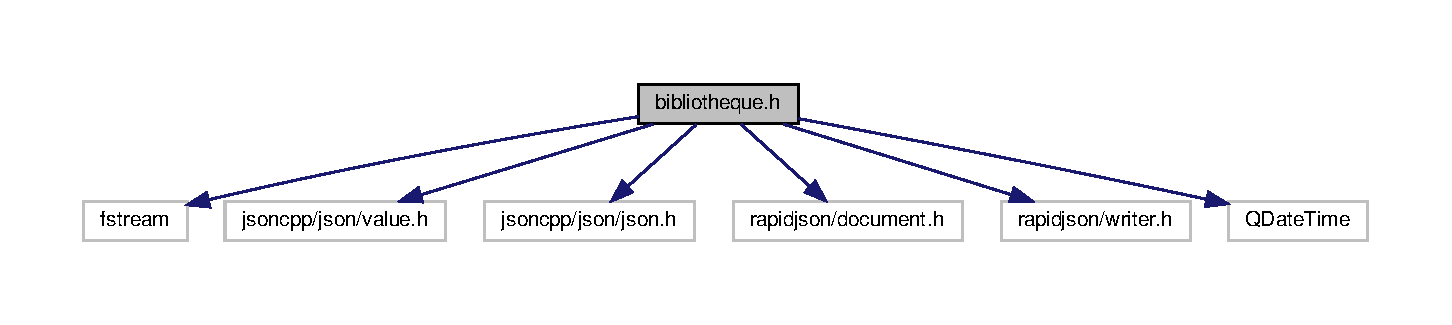
\includegraphics[width=350pt]{bibliotheque_8h__incl}
\end{center}
\end{figure}
Ce graphe montre quels fichiers incluent directement ou indirectement ce fichier \+:
\nopagebreak
\begin{figure}[H]
\begin{center}
\leavevmode
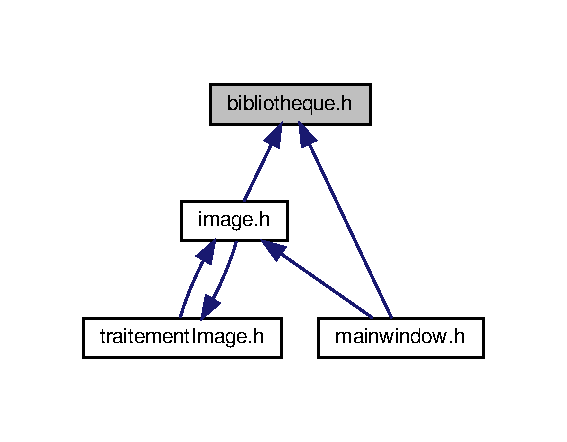
\includegraphics[width=200pt]{bibliotheque_8h__dep__incl}
\end{center}
\end{figure}
\subsection*{Classes}
\begin{DoxyCompactItemize}
\item 
class \hyperlink{classBibliotheque}{Bibliotheque}
\begin{DoxyCompactList}\small\item\em La classe \hyperlink{classBibliotheque}{Bibliotheque} permet la gestion d\textquotesingle{}une bibliotheque d\textquotesingle{}images. \end{DoxyCompactList}\end{DoxyCompactItemize}


\subsection{Description détaillée}
Header de la classe \hyperlink{classBibliotheque}{Bibliotheque}. 

\begin{DoxyVersion}{Version}
0.\+1 
\end{DoxyVersion}
\begin{DoxyDate}{Date}
2022-\/01-\/22
\end{DoxyDate}
\begin{DoxyCopyright}{Copyright}
Copyright (c) 2022 
\end{DoxyCopyright}

\hypertarget{ImageToolBox_8h}{}\section{Référence du fichier Image\+Tool\+Box.\+h}
\label{ImageToolBox_8h}\index{Image\+Tool\+Box.\+h@{Image\+Tool\+Box.\+h}}


Header du namespace Image\+Tool\+Box.  


{\ttfamily \#include $<$iostream$>$}\newline
{\ttfamily \#include $<$string$>$}\newline
{\ttfamily \#include $<$vector$>$}\newline
{\ttfamily \#include $<$fstream$>$}\newline
{\ttfamily \#include $<$algorithm$>$}\newline
{\ttfamily \#include $<$cmath$>$}\newline
{\ttfamily \#include $<$complex$>$}\newline
{\ttfamily \#include $<$jsoncpp/json/value.\+h$>$}\newline
{\ttfamily \#include $<$jsoncpp/json/json.\+h$>$}\newline
{\ttfamily \#include \char`\"{}rapidjson/document.\+h\char`\"{}}\newline
{\ttfamily \#include \char`\"{}rapidjson/writer.\+h\char`\"{}}\newline
{\ttfamily \#include $<$opencv2/core/core.\+hpp$>$}\newline
{\ttfamily \#include $<$opencv2/highgui/highgui.\+hpp$>$}\newline
{\ttfamily \#include $<$opencv2/imgproc/imgproc.\+hpp$>$}\newline
{\ttfamily \#include $<$experimental/filesystem$>$}\newline
{\ttfamily \#include \char`\"{}headers/bibliotheque.\+h\char`\"{}}\newline
Graphe des dépendances par inclusion de Image\+Tool\+Box.\+h\+:
\nopagebreak
\begin{figure}[H]
\begin{center}
\leavevmode
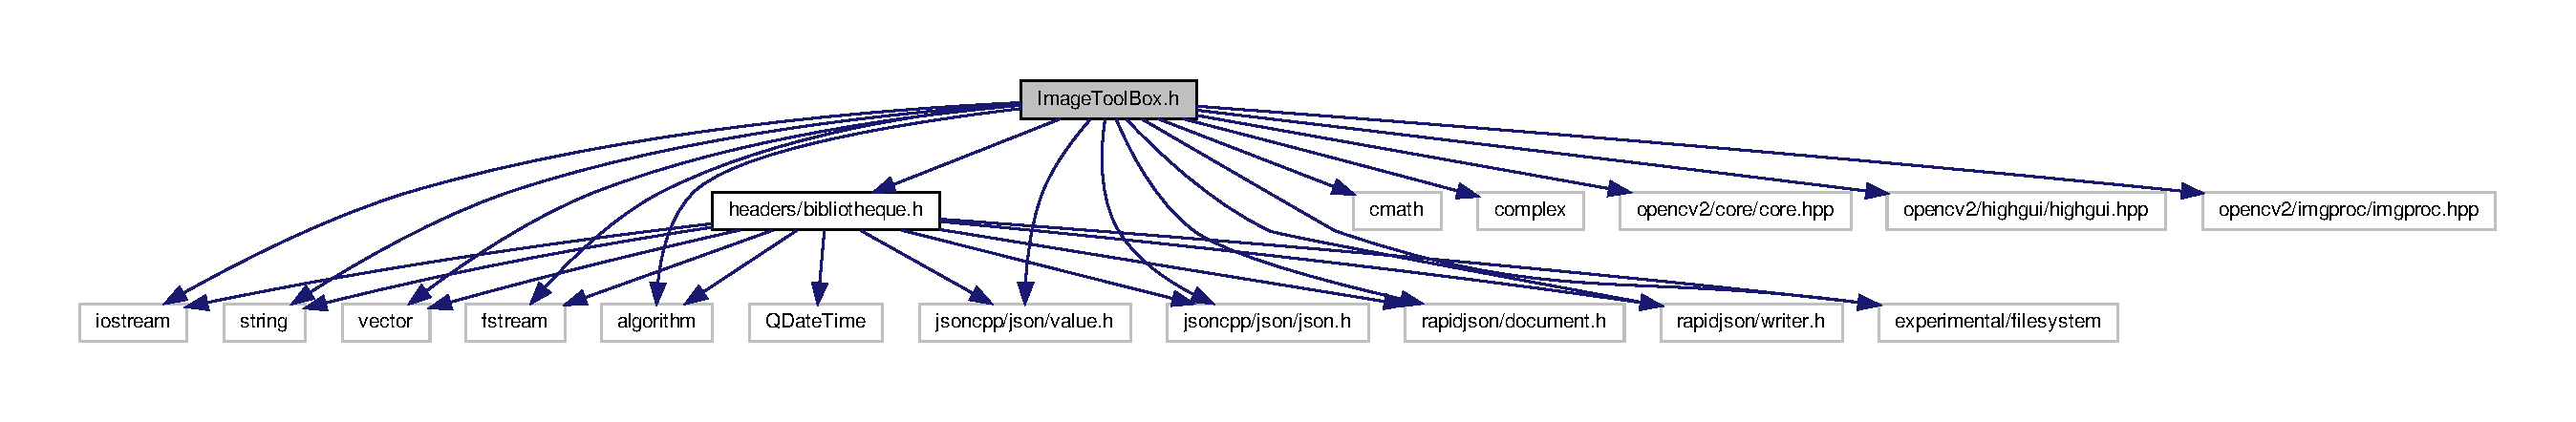
\includegraphics[width=350pt]{ImageToolBox_8h__incl}
\end{center}
\end{figure}
Ce graphe montre quels fichiers incluent directement ou indirectement ce fichier \+:
\nopagebreak
\begin{figure}[H]
\begin{center}
\leavevmode
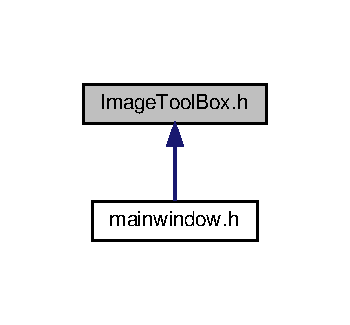
\includegraphics[width=168pt]{ImageToolBox_8h__dep__incl}
\end{center}
\end{figure}
\subsection*{Macros}
\begin{DoxyCompactItemize}
\item 
\mbox{\Hypertarget{ImageToolBox_8h_ae3b21f339690a966e921fe2545939862}\label{ImageToolBox_8h_ae3b21f339690a966e921fe2545939862}} 
\#define {\bfseries json\+\_\+char}~T\+C\+H\+AR
\end{DoxyCompactItemize}
\subsection*{Fonctions}
\begin{DoxyCompactItemize}
\item 
Mat \hyperlink{ImageToolBox_8h_addd661843fdb0c511f46875651edcbd6}{Image\+Tool\+Box\+::\+Image\+Temperature} (const Mat image, const int valeur)
\begin{DoxyCompactList}\small\item\em Ajuster la temperature de l\textquotesingle{}image. \end{DoxyCompactList}\item 
Mat \hyperlink{ImageToolBox_8h_a7d3e92ec25a4afce06055184f7756486}{Image\+Tool\+Box\+::\+Image\+Saturation} (const Mat image, const int valeur)
\begin{DoxyCompactList}\small\item\em Ajuster la saturation de l\textquotesingle{}image. \end{DoxyCompactList}\item 
Mat \hyperlink{ImageToolBox_8h_af034b8d1ea327a6439d3fed3695d2240}{Image\+Tool\+Box\+::\+Image\+Saturation\+Element} (const Mat image, const int valeur)
\begin{DoxyCompactList}\small\item\em Ajuster la saturation d\textquotesingle{}une composante de l\textquotesingle{}image. \end{DoxyCompactList}\item 
Mat \hyperlink{ImageToolBox_8h_aaf46a0ed6cb4afd5588f6b2e0ef4c7b8}{Image\+Tool\+Box\+::\+Image\+Teinte} (const Mat image, const int valeur)
\begin{DoxyCompactList}\small\item\em Ajuster la teinte de l\textquotesingle{}image. \end{DoxyCompactList}\item 
Mat \hyperlink{ImageToolBox_8h_a425a7cc2c4e74cbefba456fee2fdccde}{Image\+Tool\+Box\+::\+Image\+Vividite} (const Mat image, const int valeur)
\begin{DoxyCompactList}\small\item\em Ajuster la vividité de l\textquotesingle{}image. \end{DoxyCompactList}\item 
Mat \hyperlink{ImageToolBox_8h_af5c13d5031a214a04e534605c75e5850}{Image\+Tool\+Box\+::\+Image\+Monochrome} (const Mat image)
\begin{DoxyCompactList}\small\item\em Convertir une image en couleurs en une image en niveau de gris. \end{DoxyCompactList}\item 
Mat \hyperlink{ImageToolBox_8h_aa5ca2c6d296f029dabd1639ef6499f5d}{Image\+Tool\+Box\+::\+Image\+Sepia} (const Mat image)
\begin{DoxyCompactList}\small\item\em Appliquer un filtre de couleur sépia sur l\textquotesingle{}image. \end{DoxyCompactList}\item 
Mat \hyperlink{ImageToolBox_8h_a636100f0cf56ab824af80dce516348d6}{Image\+Tool\+Box\+::\+Image\+Inversement\+Mono} (const Mat image)
\begin{DoxyCompactList}\small\item\em Calculer la négative d\textquotesingle{}une composante de l\textquotesingle{}image de départ. \end{DoxyCompactList}\item 
Mat \hyperlink{ImageToolBox_8h_a23ade7732b5a8efcb44b7b08633ac47d}{Image\+Tool\+Box\+::\+Image\+Inversement} (const Mat image)
\begin{DoxyCompactList}\small\item\em Calculer l\textquotesingle{}image négative de l\textquotesingle{}image de départ. \end{DoxyCompactList}\item 
Mat \hyperlink{ImageToolBox_8h_aebdaf523e99806e1da3e44a90ee1c8a4}{Image\+Tool\+Box\+::\+Image\+Extraction\+Couleur} (const Mat image, int choix)
\begin{DoxyCompactList}\small\item\em Extraire une composante de couleur (R/\+V/B) de l\textquotesingle{}image. \end{DoxyCompactList}\item 
Mat \hyperlink{ImageToolBox_8h_a23b7c155298aba8b4211add64433b596}{Image\+Tool\+Box\+::\+Image\+Rouge} (const Mat image)
\begin{DoxyCompactList}\small\item\em Segmenter l\textquotesingle{}image en couleur rouge en annulant les composantes verte et bleue. \end{DoxyCompactList}\item 
Mat \hyperlink{ImageToolBox_8h_aaf314069648d59ceaf6c9a1939eb2c3c}{Image\+Tool\+Box\+::\+Image\+Vert} (const Mat image)
\begin{DoxyCompactList}\small\item\em Segmenter l\textquotesingle{}image en couleur verte en annulant les composantes rouge et bleue. \end{DoxyCompactList}\item 
Mat \hyperlink{ImageToolBox_8h_a8f31ad6d72f97d8a56472d946a85b22d}{Image\+Tool\+Box\+::\+Image\+Bleu} (const Mat image)
\begin{DoxyCompactList}\small\item\em Segmenter l\textquotesingle{}image en couleur bleue en annulant les composantes rouge et verte. \end{DoxyCompactList}\item 
Mat \hyperlink{ImageToolBox_8h_a70b7c621d8bafe9d1654b5a6e0e4b253}{Image\+Tool\+Box\+::\+Image\+Jaune} (const Mat image)
\begin{DoxyCompactList}\small\item\em Segmenter l\textquotesingle{}image en couleur jaune en annulant la composante bleue. \end{DoxyCompactList}\item 
Mat \hyperlink{ImageToolBox_8h_af2cf6ccdbc004892ab2a1092a5cefabd}{Image\+Tool\+Box\+::\+Image\+Cyan} (const Mat image)
\begin{DoxyCompactList}\small\item\em Segmenter l\textquotesingle{}image en couleur cyan en annulant la composante rouge. \end{DoxyCompactList}\item 
Mat \hyperlink{ImageToolBox_8h_a3653ad6e4ece5fd234d92909ff327610}{Image\+Tool\+Box\+::\+Image\+Magenta} (const Mat image)
\begin{DoxyCompactList}\small\item\em Segmenter l\textquotesingle{}image en couleur magenta en annulant la composante verte. \end{DoxyCompactList}\item 
Mat \hyperlink{ImageToolBox_8h_ab51b91eec0f177cd9448148e500c8c56}{Image\+Tool\+Box\+::\+Image\+R\+GB} (const Mat image)
\begin{DoxyCompactList}\small\item\em Pour chaque pixel de l\textquotesingle{}image, segmenter la composante ayant la plus grande valeur. \end{DoxyCompactList}\item 
Mat \hyperlink{ImageToolBox_8h_a67f6b69518001f06feb3f493a2bda23f}{Image\+Tool\+Box\+::\+Normalisation\+Mono} (const Mat image, const int valeur)
\begin{DoxyCompactList}\small\item\em Normaliser l\textquotesingle{}histogramme d\textquotesingle{}une composante de l\textquotesingle{}image avec intervalle réglable. \end{DoxyCompactList}\item 
Mat \hyperlink{ImageToolBox_8h_a41217fcb585826a2a94ee4ac2d75fc65}{Image\+Tool\+Box\+::\+Normalisation} (const Mat image, const int valeur)
\begin{DoxyCompactList}\small\item\em Normaliser l\textquotesingle{}histogramme de l\textquotesingle{}image avec intervalle réglable. \end{DoxyCompactList}\item 
Mat \hyperlink{ImageToolBox_8h_a24a9a180918331ed450f1ae2d37b2848}{Image\+Tool\+Box\+::\+Image\+Egalisation\+Mono} (const Mat image, const int valeur)
\begin{DoxyCompactList}\small\item\em Égaliser l\textquotesingle{}histogramme d\textquotesingle{}une composante de l\textquotesingle{}image avec nombre de pics réglable. \end{DoxyCompactList}\item 
Mat \hyperlink{ImageToolBox_8h_aa0c7afb42ac63297cbc57be5216ca611}{Image\+Tool\+Box\+::\+Image\+Egalisation} (const Mat image)
\begin{DoxyCompactList}\small\item\em Égaliser l\textquotesingle{}histogramme de l\textquotesingle{}image sur 255 pics. \end{DoxyCompactList}\item 
Mat \hyperlink{ImageToolBox_8h_a5b0402233752d5308aaa2233e60c98f9}{Image\+Tool\+Box\+::\+Image\+Luminosite} (const Mat image, const int valeur)
\begin{DoxyCompactList}\small\item\em Modifier l\textquotesingle{}intensité lumineuse de l\textquotesingle{}image en décalant son histogramme par un paramètre ajustable. \end{DoxyCompactList}\item 
Mat \hyperlink{ImageToolBox_8h_a656e1e221891d290e8c82ae66ca4c68b}{Image\+Tool\+Box\+::\+Image\+Ombre} (const Mat image, int valeur)
\begin{DoxyCompactList}\small\item\em Décaler la partie des niveaux d\textquotesingle{}intensité lumineuse inférieurs à 128 de l\textquotesingle{}histogramme de l\textquotesingle{}image en fonction d\textquotesingle{}un paramètre réglable. \end{DoxyCompactList}\item 
Mat \hyperlink{ImageToolBox_8h_a6dd26ed1096f5d37bf27fe60a3ca2457}{Image\+Tool\+Box\+::\+Image\+Haute\+Lumiere} (const Mat image, int valeur)
\begin{DoxyCompactList}\small\item\em Décaler la partie des niveaux d\textquotesingle{}intensité lumineuse supérieurs à 128 de l\textquotesingle{}histogramme de l\textquotesingle{}image en fonction d\textquotesingle{}un paramètre réglable. \end{DoxyCompactList}\item 
Mat \hyperlink{ImageToolBox_8h_aa316c5cd36631f2c48f6cd21a52d537b}{Image\+Tool\+Box\+::\+Image\+Median\+Mono} (const Mat image)
\begin{DoxyCompactList}\small\item\em Appliquer le filtre médian 3x3 sur une composante de l\textquotesingle{}image. \end{DoxyCompactList}\item 
Mat \hyperlink{ImageToolBox_8h_aebed3acea4d8f04dd863d7e4c7f6166d}{Image\+Tool\+Box\+::\+Image\+Median} (const Mat image)
\begin{DoxyCompactList}\small\item\em Appliquer un filtre médian 3x3 sur l\textquotesingle{}image de façon marginale. \end{DoxyCompactList}\item 
Mat \hyperlink{ImageToolBox_8h_a9e241aff7551628d51427e8daa5c177a}{Image\+Tool\+Box\+::\+Image\+Filtrage} (const Mat image, const int choix)
\begin{DoxyCompactList}\small\item\em Appliquer par convolution sur l\textquotesingle{}image un filtre 3x3 choisi en fonction d\textquotesingle{}un paramètre de choix. \end{DoxyCompactList}\item 
Mat \hyperlink{ImageToolBox_8h_a2e910f9392c9458c4992dc7f398389a7}{Image\+Tool\+Box\+::\+Image\+Lissage} (const Mat image, const int valeur)
\begin{DoxyCompactList}\small\item\em Lisser plusieurs fois les contours de l\textquotesingle{}image par application sucessive d\textquotesingle{}un filtre gaussien. \end{DoxyCompactList}\item 
Mat \hyperlink{ImageToolBox_8h_ac098042bb200aa93bd2c3ee655a73b73}{Image\+Tool\+Box\+::\+Image\+Kuwahara\+Mono} (const Mat image)
\begin{DoxyCompactList}\small\item\em Appliquer un filtre Kuwahara-\/\+Nagao (5x5) sur une composante de l\textquotesingle{}image. \end{DoxyCompactList}\item 
Mat \hyperlink{ImageToolBox_8h_aba41eed351a4ef55beb98aa8b7996ee0}{Image\+Tool\+Box\+::\+Image\+Kuwahara} (const Mat image)
\begin{DoxyCompactList}\small\item\em Appliquer le filtre Kuwahara-\/\+Nagao (5x5) sur l\textquotesingle{}image. \end{DoxyCompactList}\item 
Mat \hyperlink{ImageToolBox_8h_aece1e0759319d910e8e8a2ca05c67f7f}{Image\+Tool\+Box\+::\+Image\+Bruit\+Gaussien} (const Mat image, const double moyenne, const double sigma)
\begin{DoxyCompactList}\small\item\em Ajouter un bruit gaussien de moyenne et écart-\/type réglable sur l\textquotesingle{}image. \end{DoxyCompactList}\item 
Mat \hyperlink{ImageToolBox_8h_a8f6c520daae0b9cbab7d6cf0fc33c742}{Image\+Tool\+Box\+::\+Image\+Bruit\+Poivre\+Sel} (const Mat image)
\begin{DoxyCompactList}\small\item\em Bruiter l\textquotesingle{}image par un bruit poivre et sel. \end{DoxyCompactList}\item 
Mat \hyperlink{ImageToolBox_8h_af4c775b3cfe9eee037b773aa7a64457e}{Image\+Tool\+Box\+::\+Image\+Contour\+Gradient} (const Mat image)
\begin{DoxyCompactList}\small\item\em Détecter les contours dans l\textquotesingle{}image par la norme du gradient (filtres gradients 3x3) \end{DoxyCompactList}\item 
Mat \hyperlink{ImageToolBox_8h_a9e7de80e685011b2f9359c9dd71f7a73}{Image\+Tool\+Box\+::\+Image\+Contour\+Laplace} (const Mat image)
\begin{DoxyCompactList}\small\item\em Détecter les contours dans l\textquotesingle{}image par un filtre laplacien (3x3) \end{DoxyCompactList}\item 
Mat \hyperlink{ImageToolBox_8h_aea6bb5426267ff811c98091d99353b48}{Image\+Tool\+Box\+::\+Image\+Rehaussement\+Contour} (const Mat image, const int val, const int choix)
\begin{DoxyCompactList}\small\item\em Rehausser les contours de l\textquotesingle{}image en rajoutant d\textquotesingle{}une valeur d\textquotesingle{}intensité lumineuse sur les pixels des contours détéctés par un filtre choisi (3x3) \end{DoxyCompactList}\item 
Mat \hyperlink{ImageToolBox_8h_a7d1e3341d7f49b5e3a018554fb00cdea}{Image\+Tool\+Box\+::\+Image\+Seuillage} (const Mat image, const int seuil)
\begin{DoxyCompactList}\small\item\em Seuiller d\textquotesingle{}une composante de l\textquotesingle{}image avec un seui de valeur réglable. \end{DoxyCompactList}\item 
Mat \hyperlink{ImageToolBox_8h_a5ef757c9b5de9fb9d8db7eb095b84204}{Image\+Tool\+Box\+::\+Image\+Seuillage} (const Mat image, vector$<$ int $>$ seuil)
\begin{DoxyCompactList}\small\item\em Seuiller une image avec des seuils réglables pour chauqe composante. \end{DoxyCompactList}\item 
Mat \hyperlink{ImageToolBox_8h_acd44389eeda6d28216382b07233c3e4e}{Image\+Tool\+Box\+::\+Image\+Seuillage} (const Mat image, const int seuil\+Bas, const int seuil\+Haut)
\begin{DoxyCompactList}\small\item\em Seuiller de façon hystérésis une composante de l\textquotesingle{}image avec les valeurs des seuils réglables. \end{DoxyCompactList}\item 
Mat \hyperlink{ImageToolBox_8h_ae2b7c207740071d68971ce1d93d299bc}{Image\+Tool\+Box\+::\+Image\+Seuillage} (const Mat image, vector$<$ int $>$ seuil\+Bas, vector$<$ int $>$ seuil\+Haut)
\begin{DoxyCompactList}\small\item\em Seuiller de façon hystérésis une image avec les valeurs des seuils réglables pour chaque composante. \end{DoxyCompactList}\item 
Mat \hyperlink{ImageToolBox_8h_a72c917fcb65d8ecced0245200d11267d}{Image\+Tool\+Box\+::\+Image\+Segmentation} (const Mat image, const int seuil)
\begin{DoxyCompactList}\small\item\em Segmenter une composante de l\textquotesingle{}image par un seuillage simple avec la valeur du seuil réglable. \end{DoxyCompactList}\item 
Mat \hyperlink{ImageToolBox_8h_aa2e0aaa5e194a6486414858e1594bdf6}{Image\+Tool\+Box\+::\+Image\+Segmentation} (const Mat image, vector$<$ int $>$ seuil)
\begin{DoxyCompactList}\small\item\em Segmenter une image par un seuillage simple avec les valeurs des seuils réglables pour chaque composante. \end{DoxyCompactList}\item 
Mat \hyperlink{ImageToolBox_8h_a40bc78a2185a7f9401abb44602076b03}{Image\+Tool\+Box\+::\+Image\+Segmentation} (const Mat image, const int seuil\+Bas, const int seuil\+Haut)
\begin{DoxyCompactList}\small\item\em Segmenter une composante de l\textquotesingle{}image par un seuillage à hystérésis avec les valeurs des seuils réglables. \end{DoxyCompactList}\item 
Mat \hyperlink{ImageToolBox_8h_a4a2ddcf100e57cdf74a078fad7068fff}{Image\+Tool\+Box\+::\+Image\+Segmentation} (const Mat image, vector$<$ int $>$ seuil\+Bas, vector$<$ int $>$ seuil\+Haut)
\begin{DoxyCompactList}\small\item\em Segmenter une image par un seuillage à hystérésis avec les valeurs des seuils réglables pour chaque composante. \end{DoxyCompactList}\item 
Mat \hyperlink{ImageToolBox_8h_a0817ef801078f740b09029ee054ed4c1}{Image\+Tool\+Box\+::\+Image\+Quantification} (const Mat image, const int valeur)
\begin{DoxyCompactList}\small\item\em Modifier le nombre de bits à coder les intensités lumineuses de l\textquotesingle{}image. \end{DoxyCompactList}\item 
Mat \hyperlink{ImageToolBox_8h_ad3060691d16fe608aa5fcd4f715f9c8a}{Image\+Tool\+Box\+::\+Image\+Resolution\+Reduction} (const Mat image, const int valeur)
\begin{DoxyCompactList}\small\item\em Réduire la résolution d\textquotesingle{}une image par sous-\/échantillonnage. \end{DoxyCompactList}\item 
Mat \hyperlink{ImageToolBox_8h_accb8d215c8b6516f9029875db9f2a128}{Image\+Tool\+Box\+::\+Interpolation\+P\+PP} (const Mat image, const int valeur)
\begin{DoxyCompactList}\small\item\em Augmenter la résolution d\textquotesingle{}une image par interpolation par pixel le plus proche. \end{DoxyCompactList}\item 
Mat \hyperlink{ImageToolBox_8h_af622a53adfeb58fe99d171a427162686}{Image\+Tool\+Box\+::\+Interpolation\+Bilineaire} (const Mat image, const int valeur)
\begin{DoxyCompactList}\small\item\em Augmenter la résolution d\textquotesingle{}une image par interpolation bilinéaire. \end{DoxyCompactList}\item 
Mat \hyperlink{ImageToolBox_8h_a949347b021d7a4b1886ca20dea09d8f1}{Image\+Tool\+Box\+::\+Interpolation\+Bilineaire\+Mono} (const Mat image, const int valeur)
\begin{DoxyCompactList}\small\item\em Augmenter la résolution d\textquotesingle{}une composante de l\textquotesingle{}image par interpolation bilinéaire. \end{DoxyCompactList}\item 
int \hyperlink{ImageToolBox_8h_af4723186573a960f2e40a7794a8a2843}{Image\+Tool\+Box\+::\+Min\+Image} (const Mat image)
\begin{DoxyCompactList}\small\item\em Déterminer la valeur minimale d\textquotesingle{}une matrice de type entier. \end{DoxyCompactList}\item 
int \hyperlink{ImageToolBox_8h_ad3f83f15fa84a972418caecd26014cc0}{Image\+Tool\+Box\+::\+Max\+Image} (const Mat image)
\begin{DoxyCompactList}\small\item\em Déterminer la valeur maximale d\textquotesingle{}une matrice de type entier. \end{DoxyCompactList}\item 
double \hyperlink{ImageToolBox_8h_a0fb0fd1d1ee00e522de2544f1e938b1c}{Image\+Tool\+Box\+::\+Min\+Vecteur} (const vector$<$ double $>$ vecteur)
\begin{DoxyCompactList}\small\item\em Déterminer la valeur minimale d\textquotesingle{}un vecteur de type réel. \end{DoxyCompactList}\item 
double \hyperlink{ImageToolBox_8h_a47cfca23f6ecfa9b039e036d23280722}{Image\+Tool\+Box\+::\+Max\+Vecteur} (const vector$<$ double $>$ vecteur)
\begin{DoxyCompactList}\small\item\em Déterminer la valeur maximale d\textquotesingle{}un vecteur de type réel. \end{DoxyCompactList}\item 
int \hyperlink{ImageToolBox_8h_aac980b1ad3c55e5ce18dc43a867d56e5}{Image\+Tool\+Box\+::\+Min\+Vecteur} (const vector$<$ int $>$ vecteur)
\begin{DoxyCompactList}\small\item\em Déterminer la valeur minimale d\textquotesingle{}un vecteur de type entier. \end{DoxyCompactList}\item 
int \hyperlink{ImageToolBox_8h_a67040c0394a74803361ff86dd0331a27}{Image\+Tool\+Box\+::\+Max\+Vecteur} (const vector$<$ int $>$ vecteur)
\begin{DoxyCompactList}\small\item\em Déterminer la valeur maximale d\textquotesingle{}un vecteur de type entier. \end{DoxyCompactList}\item 
int \hyperlink{ImageToolBox_8h_aa66d565bea8f8e8d3490cdf1eeb2eb3a}{Image\+Tool\+Box\+::\+Min\+Vecteur\+Indice} (const vector$<$ int $>$ vecteur)
\begin{DoxyCompactList}\small\item\em Déterminer l\textquotesingle{}indice de la valeur minimale d\textquotesingle{}un vecteur de type entier. \end{DoxyCompactList}\item 
int \hyperlink{ImageToolBox_8h_a9dc4b2ebdc57ab762baef8078179b4ea}{Image\+Tool\+Box\+::\+Min\+Vecteur\+Indice} (const vector$<$ double $>$ vecteur)
\begin{DoxyCompactList}\small\item\em Déterminer l\textquotesingle{}indice de la valeur minimale d\textquotesingle{}un vecteur de type réel. \end{DoxyCompactList}\item 
vector$<$ int $>$ \hyperlink{ImageToolBox_8h_a1282e097d7e2138715ef3b30f9a4ac04}{Image\+Tool\+Box\+::\+Histogramme} (const Mat image, const int nb\+Intervalle)
\begin{DoxyCompactList}\small\item\em Calculer l\textquotesingle{}histogramme d\textquotesingle{}une image avec le nombre d\textquotesingle{}intervalles réglable. \end{DoxyCompactList}\item 
vector$<$ int $>$ \hyperlink{ImageToolBox_8h_a52c9a676a7649169f62d8c49ad95fed8}{Image\+Tool\+Box\+::\+Egalisation} (const Mat image, const int nb\+Intervalle)
\begin{DoxyCompactList}\small\item\em Égaliser d\textquotesingle{}un histogramme sur un nombre d\textquotesingle{}intervalles réglable. \end{DoxyCompactList}\item 
Mat \hyperlink{ImageToolBox_8h_a6eb6ef6eb2bf6b706d3c14eb66aae2e9}{Image\+Tool\+Box\+::\+Image\+Zero} (const int nb\+Ligne, const int nb\+Colonne)
\begin{DoxyCompactList}\small\item\em Générer une matrice de dimensions choisies contenant que des zéros. \end{DoxyCompactList}\item 
Mat \hyperlink{ImageToolBox_8h_a66616f84939e8938f1c770ace712f820}{Image\+Tool\+Box\+::\+Matrice\+Convolution} (const Mat image, const Mat filtre)
\begin{DoxyCompactList}\small\item\em Effectuer un produit de convolution entre une composante de l\textquotesingle{}image et un filtre. \end{DoxyCompactList}\item 
Mat \hyperlink{ImageToolBox_8h_ad43a6426bc7207910c46c9a29d637039}{Image\+Tool\+Box\+::\+Image\+Convolution} (const Mat image, const Mat filtre)
\begin{DoxyCompactList}\small\item\em Effectuer un produit de convolution entre une image et un filtre. \end{DoxyCompactList}\item 
Mat \hyperlink{ImageToolBox_8h_a001917bd10eeaaeed211e8e7922ce382}{Image\+Tool\+Box\+::\+Matrice\+Norme} (const Mat imageX, const Mat imageY)
\begin{DoxyCompactList}\small\item\em Calculer la norme d\textquotesingle{}une image avec leurs gradients dans les deux directions horizontale et verticale. \end{DoxyCompactList}\item 
Mat \hyperlink{ImageToolBox_8h_a240834ef283230eb6f72c5cef309f131}{Image\+Tool\+Box\+::\+GradientX} (const Mat image, const string type\+Filtre)
\begin{DoxyCompactList}\small\item\em Calculer le gradient de l\textquotesingle{}image dans la direction horizontale. \end{DoxyCompactList}\item 
Mat \hyperlink{ImageToolBox_8h_aa128c57048bb745f88739a1fc4452176}{Image\+Tool\+Box\+::\+GradientY} (const Mat image, const string type\+Filtre)
\begin{DoxyCompactList}\small\item\em Calculer le gradient de l\textquotesingle{}image dans la direction verticale. \end{DoxyCompactList}\item 
Mat \hyperlink{ImageToolBox_8h_a0407f85e7cd66d102507b6b6703c113b}{Image\+Tool\+Box\+::\+Max\+Norme\+Gradient} (const Mat gradient\+Norme, const Mat gradientX, const Mat gradientY)
\begin{DoxyCompactList}\small\item\em Déterminer le maximum de la norme du gradient dans la direction du gradient de l\textquotesingle{}image. \end{DoxyCompactList}\item 
int \hyperlink{ImageToolBox_8h_a5a502550eb3e4f7fd755846d514c595e}{Image\+Tool\+Box\+::\+Matrice\+Median} (const Mat matrice)
\begin{DoxyCompactList}\small\item\em Déterminer la valeur médiane d\textquotesingle{}une matrice (dimensions quelconques) \end{DoxyCompactList}\item 
int \hyperlink{ImageToolBox_8h_a62e96cbe37c9a36356c49ae2471d8162}{Image\+Tool\+Box\+::\+Vecteur\+Median} (vector$<$ int $>$ vecteur)
\begin{DoxyCompactList}\small\item\em Déterminer la valeur médiane d\textquotesingle{}un vecteur. \end{DoxyCompactList}\item 
bool \hyperlink{ImageToolBox_8h_ac1c51a943b34b1a95e552d7ea35164c5}{Image\+Tool\+Box\+::\+Matrice\+Egale} (const Mat matrice1, const Mat matrice2)
\begin{DoxyCompactList}\small\item\em Vérifier l\textquotesingle{}égalité entre deux matrices de mêmes dimensions. \end{DoxyCompactList}\item 
double \hyperlink{ImageToolBox_8h_a7e6f0e6794cbcfd301b2a4598971df10}{Image\+Tool\+Box\+::\+Moyenne\+Vecteur} (const vector$<$ double $>$ vecteur)
\begin{DoxyCompactList}\small\item\em Calculer la moyenne des valeurs d\textquotesingle{}un vecteur réel. \end{DoxyCompactList}\item 
double \hyperlink{ImageToolBox_8h_a3ff5538fa3264135cfeb09bc62842575}{Image\+Tool\+Box\+::\+Variance\+Vecteur} (const vector$<$ double $>$ vecteur)
\begin{DoxyCompactList}\small\item\em Calculer la variance des valeurs d\textquotesingle{}un vecteur réel. \end{DoxyCompactList}\item 
Mat \hyperlink{ImageToolBox_8h_ad2b9c41615174a35b085a12592585945}{Image\+Tool\+Box\+::\+Image\+Fourier} (const Mat image)
\begin{DoxyCompactList}\small\item\em Calculer la trasformée de Fourier 2D d\textquotesingle{}une image. \end{DoxyCompactList}\item 
double \hyperlink{ImageToolBox_8h_abf17386fd4690999a5dc7e692569cb37}{Image\+Tool\+Box\+::\+Image\+Fourier\+Element} (const Mat image, const int ligne, const int colonne)
\begin{DoxyCompactList}\small\item\em Calculer la transformée de Fourier 2D d\textquotesingle{}un pixel de l\textquotesingle{}image. \end{DoxyCompactList}\item 
Mat \hyperlink{ImageToolBox_8h_a5e4daf19045b95550849550a9f0b4c42}{Image\+Tool\+Box\+::\+Image\+Miroir} (const Mat image, const Mat filtre)
\begin{DoxyCompactList}\small\item\em Effectuer l\textquotesingle{}effet miroir sur une image en basant sur ses dimensions et les dimensions du filtre à appliquer sur l\textquotesingle{}image. \end{DoxyCompactList}\item 
Mat \hyperlink{ImageToolBox_8h_a4382368a70d6b3fff646ae456ca5d27a}{Image\+Tool\+Box\+::\+Image\+Miroir} (const Mat image, const int taille)
\begin{DoxyCompactList}\small\item\em Effectuer l\textquotesingle{}effet miroir sur une image avec un voisinage carré de taille quelconque. \end{DoxyCompactList}\item 
Mat \hyperlink{ImageToolBox_8h_a03a2008c61fe17fc9e027430dc06bb5c}{Image\+Tool\+Box\+::\+Generer\+Filtre} (const int type\+Filtre)
\begin{DoxyCompactList}\small\item\em Générer un filtre 3x3 selon le type de filtre choisi. \end{DoxyCompactList}\item 
Mat \hyperlink{ImageToolBox_8h_a32ae36b60559b8a5d598e5c52c396099}{Image\+Tool\+Box\+::\+Mono\+Couleur} (const Mat image)
\begin{DoxyCompactList}\small\item\em Transformer une composante de l\textquotesingle{}image en une image de trois composantes identiques. \end{DoxyCompactList}\item 
Mat \hyperlink{ImageToolBox_8h_a65d057dcccb22865659761f5ffe0f53b}{Image\+Tool\+Box\+::\+Plot\+Histogram1D} (Mat image, int choix\+Couleur)
\begin{DoxyCompactList}\small\item\em Calculer et tracer l\textquotesingle{}histogramme d\textquotesingle{}une composante choisie de l\textquotesingle{}image. \end{DoxyCompactList}\item 
Mat \hyperlink{ImageToolBox_8h_aec42a04516c264072abb2ee810b5c8df}{Image\+Tool\+Box\+::\+Calc\+Histogram} (Mat image)
\begin{DoxyCompactList}\small\item\em Calculer l\textquotesingle{}histogramme de l\textquotesingle{}image. \end{DoxyCompactList}\item 
Mat \hyperlink{ImageToolBox_8h_a3e6d89d93444def9ea01401db360e704}{Image\+Tool\+Box\+::\+Plot\+Histogram} (Mat image)
\begin{DoxyCompactList}\small\item\em Plot\+Histogram. \end{DoxyCompactList}\item 
bool \hyperlink{ImageToolBox_8h_a28a646856e89ea75411ed960622ff8ae}{Image\+Tool\+Box\+::\+Verifier\+Image} (const Mat image, Mat \&image\+Verifiee)
\begin{DoxyCompactList}\small\item\em Vérifier si une image est en niveau de gris. \end{DoxyCompactList}\item 
Mat \hyperlink{ImageToolBox_8h_a996455b582ed88d1003d0f7cfd08135a}{Image\+Tool\+Box\+::\+Image\+B\+G\+R\+R\+GB} (const Mat image)
\begin{DoxyCompactList}\small\item\em Réarranger les composantes de l\textquotesingle{}image de B\+GR vers R\+GB. \end{DoxyCompactList}\item 
int \hyperlink{ImageToolBox_8h_aeb0a18c2585e268d0e3eec18e29e9ecb}{Image\+Tool\+Box\+::\+Verifier\+Saturation} (const int valeur)
\begin{DoxyCompactList}\small\item\em Vérifier la saturation de la valeur d\textquotesingle{}un pixel de l\textquotesingle{}image. \end{DoxyCompactList}\item 
Mat \hyperlink{ImageToolBox_8h_add7af4ead9829a856b445e291318994e}{Image\+Tool\+Box\+::\+Image\+Fourier\+Arranger} (const Mat image)
\begin{DoxyCompactList}\small\item\em Arranger la représentation de la transformee de Fourier 2D de l\textquotesingle{}image. \end{DoxyCompactList}\end{DoxyCompactItemize}


\subsection{Description détaillée}
Header du namespace Image\+Tool\+Box. 

\begin{DoxyVersion}{Version}
0.\+1 
\end{DoxyVersion}
\begin{DoxyDate}{Date}
2022-\/01-\/22
\end{DoxyDate}
\begin{DoxyCopyright}{Copyright}
Copyright (c) 2022 
\end{DoxyCopyright}


\subsection{Documentation des fonctions}
\mbox{\Hypertarget{ImageToolBox_8h_file_aec42a04516c264072abb2ee810b5c8df}\label{ImageToolBox_8h_file_aec42a04516c264072abb2ee810b5c8df}} 
\index{Image\+Tool\+Box.\+h@{Image\+Tool\+Box.\+h}!Calc\+Histogram@{Calc\+Histogram}}
\index{Calc\+Histogram@{Calc\+Histogram}!Image\+Tool\+Box.\+h@{Image\+Tool\+Box.\+h}}
\subsubsection{\texorpdfstring{Calc\+Histogram()}{CalcHistogram()}}
{\footnotesize\ttfamily Mat Image\+Tool\+Box\+::\+Calc\+Histogram (\begin{DoxyParamCaption}\item[{Mat}]{image }\end{DoxyParamCaption})}



Calculer l\textquotesingle{}histogramme de l\textquotesingle{}image. 


\begin{DoxyParams}{Paramètres}
{\em image} & Image à calculer son histogramme \\
\hline
\end{DoxyParams}
\begin{DoxyReturn}{Renvoie}

\end{DoxyReturn}
\mbox{\Hypertarget{ImageToolBox_8h_file_a52c9a676a7649169f62d8c49ad95fed8}\label{ImageToolBox_8h_file_a52c9a676a7649169f62d8c49ad95fed8}} 
\index{Image\+Tool\+Box.\+h@{Image\+Tool\+Box.\+h}!Egalisation@{Egalisation}}
\index{Egalisation@{Egalisation}!Image\+Tool\+Box.\+h@{Image\+Tool\+Box.\+h}}
\subsubsection{\texorpdfstring{Egalisation()}{Egalisation()}}
{\footnotesize\ttfamily vector$<$int$>$ Image\+Tool\+Box\+::\+Egalisation (\begin{DoxyParamCaption}\item[{const Mat}]{image,  }\item[{const int}]{nb\+Intervalle }\end{DoxyParamCaption})}



Égaliser d\textquotesingle{}un histogramme sur un nombre d\textquotesingle{}intervalles réglable. 


\begin{DoxyParams}{Paramètres}
{\em image} & Image de départ (dimensions quelconques) \\
\hline
{\em nb\+Intervalle} & Nombre d\textquotesingle{}intervalles à égaliser \\
\hline
\end{DoxyParams}
\begin{DoxyReturn}{Renvoie}
Occurences de l\textquotesingle{}histogramme égalisé 
\end{DoxyReturn}
\mbox{\Hypertarget{ImageToolBox_8h_file_a03a2008c61fe17fc9e027430dc06bb5c}\label{ImageToolBox_8h_file_a03a2008c61fe17fc9e027430dc06bb5c}} 
\index{Image\+Tool\+Box.\+h@{Image\+Tool\+Box.\+h}!Generer\+Filtre@{Generer\+Filtre}}
\index{Generer\+Filtre@{Generer\+Filtre}!Image\+Tool\+Box.\+h@{Image\+Tool\+Box.\+h}}
\subsubsection{\texorpdfstring{Generer\+Filtre()}{GenererFiltre()}}
{\footnotesize\ttfamily Mat Image\+Tool\+Box\+::\+Generer\+Filtre (\begin{DoxyParamCaption}\item[{const int}]{type\+Filtre }\end{DoxyParamCaption})}



Générer un filtre 3x3 selon le type de filtre choisi. 


\begin{DoxyParams}{Paramètres}
{\em type\+Filtre} & Type du filtre (3x3) à générer \+: 1-\/\+Moyenneur, 2-\/\+Laplacien, 3-\/\+Gaussien, 4-\/\+Gradient horizontal (Sobel), 5-\/\+Gradient vertical (Sobel), 6-\/\+Gradient horizontl (définition), 7-\/\+Gradient vertical (définition) \\
\hline
\end{DoxyParams}
\begin{DoxyReturn}{Renvoie}
Filtre 3x3 correspondant au type choisi 
\end{DoxyReturn}
\mbox{\Hypertarget{ImageToolBox_8h_file_a240834ef283230eb6f72c5cef309f131}\label{ImageToolBox_8h_file_a240834ef283230eb6f72c5cef309f131}} 
\index{Image\+Tool\+Box.\+h@{Image\+Tool\+Box.\+h}!GradientX@{GradientX}}
\index{GradientX@{GradientX}!Image\+Tool\+Box.\+h@{Image\+Tool\+Box.\+h}}
\subsubsection{\texorpdfstring{Gradient\+X()}{GradientX()}}
{\footnotesize\ttfamily Mat Image\+Tool\+Box\+::\+GradientX (\begin{DoxyParamCaption}\item[{const Mat}]{image,  }\item[{const string}]{type\+Filtre }\end{DoxyParamCaption})}



Calculer le gradient de l\textquotesingle{}image dans la direction horizontale. 


\begin{DoxyParams}{Paramètres}
{\em image} & Image de départ (dimensions quelconques) \\
\hline
{\em type\+Filtre} & Type de filtre gradient horizontal (3x3) \+: \char`\"{}\+Simple\char`\"{}-\/\+Filtre gradient par définition, \char`\"{}\+Sobel\char`\"{}-\/\+Filtre gradient de Sobel \\
\hline
\end{DoxyParams}
\begin{DoxyReturn}{Renvoie}
Gradient de l\textquotesingle{}image dans la direction horizontale 
\end{DoxyReturn}
\mbox{\Hypertarget{ImageToolBox_8h_file_aa128c57048bb745f88739a1fc4452176}\label{ImageToolBox_8h_file_aa128c57048bb745f88739a1fc4452176}} 
\index{Image\+Tool\+Box.\+h@{Image\+Tool\+Box.\+h}!GradientY@{GradientY}}
\index{GradientY@{GradientY}!Image\+Tool\+Box.\+h@{Image\+Tool\+Box.\+h}}
\subsubsection{\texorpdfstring{Gradient\+Y()}{GradientY()}}
{\footnotesize\ttfamily Mat Image\+Tool\+Box\+::\+GradientY (\begin{DoxyParamCaption}\item[{const Mat}]{image,  }\item[{const string}]{type\+Filtre }\end{DoxyParamCaption})}



Calculer le gradient de l\textquotesingle{}image dans la direction verticale. 


\begin{DoxyParams}{Paramètres}
{\em image} & Image de départ (dimensions quelconques) \\
\hline
{\em type\+Filtre} & Type de filtre gradient vertical (3x3) \+: \char`\"{}\+Simple\char`\"{}-\/\+Filtre gradient par définition, \char`\"{}\+Sobel\char`\"{}-\/\+Filtre gradient de Sobel \\
\hline
\end{DoxyParams}
\begin{DoxyReturn}{Renvoie}
Gradient de l\textquotesingle{}image dans la direction verticale 
\end{DoxyReturn}
\mbox{\Hypertarget{ImageToolBox_8h_file_a1282e097d7e2138715ef3b30f9a4ac04}\label{ImageToolBox_8h_file_a1282e097d7e2138715ef3b30f9a4ac04}} 
\index{Image\+Tool\+Box.\+h@{Image\+Tool\+Box.\+h}!Histogramme@{Histogramme}}
\index{Histogramme@{Histogramme}!Image\+Tool\+Box.\+h@{Image\+Tool\+Box.\+h}}
\subsubsection{\texorpdfstring{Histogramme()}{Histogramme()}}
{\footnotesize\ttfamily vector$<$int$>$ Image\+Tool\+Box\+::\+Histogramme (\begin{DoxyParamCaption}\item[{const Mat}]{image,  }\item[{const int}]{nb\+Intervalle }\end{DoxyParamCaption})}



Calculer l\textquotesingle{}histogramme d\textquotesingle{}une image avec le nombre d\textquotesingle{}intervalles réglable. 


\begin{DoxyParams}{Paramètres}
{\em image} & Image à calculer l\textquotesingle{}histogramme \\
\hline
{\em nb\+Intervalle} & Nombre d\textquotesingle{}intervalle de l\textquotesingle{}histogramme \\
\hline
\end{DoxyParams}
\begin{DoxyReturn}{Renvoie}
Occurences de l\textquotesingle{}histogramme de l\textquotesingle{}image 
\end{DoxyReturn}
\mbox{\Hypertarget{ImageToolBox_8h_file_a996455b582ed88d1003d0f7cfd08135a}\label{ImageToolBox_8h_file_a996455b582ed88d1003d0f7cfd08135a}} 
\index{Image\+Tool\+Box.\+h@{Image\+Tool\+Box.\+h}!Image\+B\+G\+R\+R\+GB@{Image\+B\+G\+R\+R\+GB}}
\index{Image\+B\+G\+R\+R\+GB@{Image\+B\+G\+R\+R\+GB}!Image\+Tool\+Box.\+h@{Image\+Tool\+Box.\+h}}
\subsubsection{\texorpdfstring{Image\+B\+G\+R\+R\+G\+B()}{ImageBGRRGB()}}
{\footnotesize\ttfamily Mat Image\+Tool\+Box\+::\+Image\+B\+G\+R\+R\+GB (\begin{DoxyParamCaption}\item[{const Mat}]{image }\end{DoxyParamCaption})}



Réarranger les composantes de l\textquotesingle{}image de B\+GR vers R\+GB. 


\begin{DoxyParams}{Paramètres}
{\em image} & Image de départ \\
\hline
\end{DoxyParams}
\begin{DoxyReturn}{Renvoie}
Image avec les composantes réarrangées 
\end{DoxyReturn}
\mbox{\Hypertarget{ImageToolBox_8h_file_a8f31ad6d72f97d8a56472d946a85b22d}\label{ImageToolBox_8h_file_a8f31ad6d72f97d8a56472d946a85b22d}} 
\index{Image\+Tool\+Box.\+h@{Image\+Tool\+Box.\+h}!Image\+Bleu@{Image\+Bleu}}
\index{Image\+Bleu@{Image\+Bleu}!Image\+Tool\+Box.\+h@{Image\+Tool\+Box.\+h}}
\subsubsection{\texorpdfstring{Image\+Bleu()}{ImageBleu()}}
{\footnotesize\ttfamily Mat Image\+Tool\+Box\+::\+Image\+Bleu (\begin{DoxyParamCaption}\item[{const Mat}]{image }\end{DoxyParamCaption})}



Segmenter l\textquotesingle{}image en couleur bleue en annulant les composantes rouge et verte. 


\begin{DoxyParams}{Paramètres}
{\em image} & Image de départ (dimensions quelconques) \\
\hline
\end{DoxyParams}
\begin{DoxyReturn}{Renvoie}
Image segmentée en couleur bleue 
\end{DoxyReturn}
\mbox{\Hypertarget{ImageToolBox_8h_file_aece1e0759319d910e8e8a2ca05c67f7f}\label{ImageToolBox_8h_file_aece1e0759319d910e8e8a2ca05c67f7f}} 
\index{Image\+Tool\+Box.\+h@{Image\+Tool\+Box.\+h}!Image\+Bruit\+Gaussien@{Image\+Bruit\+Gaussien}}
\index{Image\+Bruit\+Gaussien@{Image\+Bruit\+Gaussien}!Image\+Tool\+Box.\+h@{Image\+Tool\+Box.\+h}}
\subsubsection{\texorpdfstring{Image\+Bruit\+Gaussien()}{ImageBruitGaussien()}}
{\footnotesize\ttfamily Mat Image\+Tool\+Box\+::\+Image\+Bruit\+Gaussien (\begin{DoxyParamCaption}\item[{const Mat}]{image,  }\item[{const double}]{moyenne,  }\item[{const double}]{sigma }\end{DoxyParamCaption})}



Ajouter un bruit gaussien de moyenne et écart-\/type réglable sur l\textquotesingle{}image. 


\begin{DoxyParams}{Paramètres}
{\em image} & Image de départ (dimensions quelconques) \\
\hline
{\em moyenne} & Moyenne du bruit \\
\hline
{\em sigma} & Écart-\/type du bruit \\
\hline
\end{DoxyParams}
\begin{DoxyReturn}{Renvoie}
Image bruitée par le bruit gaussien paramétré 
\end{DoxyReturn}
\mbox{\Hypertarget{ImageToolBox_8h_file_a8f6c520daae0b9cbab7d6cf0fc33c742}\label{ImageToolBox_8h_file_a8f6c520daae0b9cbab7d6cf0fc33c742}} 
\index{Image\+Tool\+Box.\+h@{Image\+Tool\+Box.\+h}!Image\+Bruit\+Poivre\+Sel@{Image\+Bruit\+Poivre\+Sel}}
\index{Image\+Bruit\+Poivre\+Sel@{Image\+Bruit\+Poivre\+Sel}!Image\+Tool\+Box.\+h@{Image\+Tool\+Box.\+h}}
\subsubsection{\texorpdfstring{Image\+Bruit\+Poivre\+Sel()}{ImageBruitPoivreSel()}}
{\footnotesize\ttfamily Mat Image\+Tool\+Box\+::\+Image\+Bruit\+Poivre\+Sel (\begin{DoxyParamCaption}\item[{const Mat}]{image }\end{DoxyParamCaption})}



Bruiter l\textquotesingle{}image par un bruit poivre et sel. 


\begin{DoxyParams}{Paramètres}
{\em image} & Image de départ (dimensions quelconques) \\
\hline
\end{DoxyParams}
\begin{DoxyReturn}{Renvoie}
Image bruitée par le bruit poivre et sel 
\end{DoxyReturn}
\mbox{\Hypertarget{ImageToolBox_8h_file_af4c775b3cfe9eee037b773aa7a64457e}\label{ImageToolBox_8h_file_af4c775b3cfe9eee037b773aa7a64457e}} 
\index{Image\+Tool\+Box.\+h@{Image\+Tool\+Box.\+h}!Image\+Contour\+Gradient@{Image\+Contour\+Gradient}}
\index{Image\+Contour\+Gradient@{Image\+Contour\+Gradient}!Image\+Tool\+Box.\+h@{Image\+Tool\+Box.\+h}}
\subsubsection{\texorpdfstring{Image\+Contour\+Gradient()}{ImageContourGradient()}}
{\footnotesize\ttfamily Mat Image\+Tool\+Box\+::\+Image\+Contour\+Gradient (\begin{DoxyParamCaption}\item[{const Mat}]{image }\end{DoxyParamCaption})}



Détecter les contours dans l\textquotesingle{}image par la norme du gradient (filtres gradients 3x3) 


\begin{DoxyParams}{Paramètres}
{\em image} & Image de départ (dimensions quelconques) \\
\hline
\end{DoxyParams}
\begin{DoxyReturn}{Renvoie}
Image des contours dans l\textquotesingle{}image de départ 
\end{DoxyReturn}
\mbox{\Hypertarget{ImageToolBox_8h_file_a9e7de80e685011b2f9359c9dd71f7a73}\label{ImageToolBox_8h_file_a9e7de80e685011b2f9359c9dd71f7a73}} 
\index{Image\+Tool\+Box.\+h@{Image\+Tool\+Box.\+h}!Image\+Contour\+Laplace@{Image\+Contour\+Laplace}}
\index{Image\+Contour\+Laplace@{Image\+Contour\+Laplace}!Image\+Tool\+Box.\+h@{Image\+Tool\+Box.\+h}}
\subsubsection{\texorpdfstring{Image\+Contour\+Laplace()}{ImageContourLaplace()}}
{\footnotesize\ttfamily Mat Image\+Tool\+Box\+::\+Image\+Contour\+Laplace (\begin{DoxyParamCaption}\item[{const Mat}]{image }\end{DoxyParamCaption})}



Détecter les contours dans l\textquotesingle{}image par un filtre laplacien (3x3) 


\begin{DoxyParams}{Paramètres}
{\em image} & Image de départ (dimensions quelconques) \\
\hline
\end{DoxyParams}
\begin{DoxyReturn}{Renvoie}
Image des contours dans l\textquotesingle{}image de départ 
\end{DoxyReturn}
\mbox{\Hypertarget{ImageToolBox_8h_file_ad43a6426bc7207910c46c9a29d637039}\label{ImageToolBox_8h_file_ad43a6426bc7207910c46c9a29d637039}} 
\index{Image\+Tool\+Box.\+h@{Image\+Tool\+Box.\+h}!Image\+Convolution@{Image\+Convolution}}
\index{Image\+Convolution@{Image\+Convolution}!Image\+Tool\+Box.\+h@{Image\+Tool\+Box.\+h}}
\subsubsection{\texorpdfstring{Image\+Convolution()}{ImageConvolution()}}
{\footnotesize\ttfamily Mat Image\+Tool\+Box\+::\+Image\+Convolution (\begin{DoxyParamCaption}\item[{const Mat}]{image,  }\item[{const Mat}]{filtre }\end{DoxyParamCaption})}



Effectuer un produit de convolution entre une image et un filtre. 


\begin{DoxyParams}{Paramètres}
{\em image} & Image de départ (dimensions quelconques) \\
\hline
{\em filtre} & Filtre (dimensions quelconques) \\
\hline
\end{DoxyParams}
\begin{DoxyReturn}{Renvoie}
Image convoluée par le filtre 
\end{DoxyReturn}
\mbox{\Hypertarget{ImageToolBox_8h_file_af2cf6ccdbc004892ab2a1092a5cefabd}\label{ImageToolBox_8h_file_af2cf6ccdbc004892ab2a1092a5cefabd}} 
\index{Image\+Tool\+Box.\+h@{Image\+Tool\+Box.\+h}!Image\+Cyan@{Image\+Cyan}}
\index{Image\+Cyan@{Image\+Cyan}!Image\+Tool\+Box.\+h@{Image\+Tool\+Box.\+h}}
\subsubsection{\texorpdfstring{Image\+Cyan()}{ImageCyan()}}
{\footnotesize\ttfamily Mat Image\+Tool\+Box\+::\+Image\+Cyan (\begin{DoxyParamCaption}\item[{const Mat}]{image }\end{DoxyParamCaption})}



Segmenter l\textquotesingle{}image en couleur cyan en annulant la composante rouge. 


\begin{DoxyParams}{Paramètres}
{\em image} & Image de départ (dimensions quelconques) \\
\hline
\end{DoxyParams}
\begin{DoxyReturn}{Renvoie}
Image segmentée en couleur cyan 
\end{DoxyReturn}
\mbox{\Hypertarget{ImageToolBox_8h_file_aa0c7afb42ac63297cbc57be5216ca611}\label{ImageToolBox_8h_file_aa0c7afb42ac63297cbc57be5216ca611}} 
\index{Image\+Tool\+Box.\+h@{Image\+Tool\+Box.\+h}!Image\+Egalisation@{Image\+Egalisation}}
\index{Image\+Egalisation@{Image\+Egalisation}!Image\+Tool\+Box.\+h@{Image\+Tool\+Box.\+h}}
\subsubsection{\texorpdfstring{Image\+Egalisation()}{ImageEgalisation()}}
{\footnotesize\ttfamily Mat Image\+Tool\+Box\+::\+Image\+Egalisation (\begin{DoxyParamCaption}\item[{const Mat}]{image }\end{DoxyParamCaption})}



Égaliser l\textquotesingle{}histogramme de l\textquotesingle{}image sur 255 pics. 


\begin{DoxyParams}{Paramètres}
{\em image} & Image de départ (dimensions quelconques) \\
\hline
\end{DoxyParams}
\begin{DoxyReturn}{Renvoie}
Image avec histogramme égalisé 
\end{DoxyReturn}
\mbox{\Hypertarget{ImageToolBox_8h_file_a24a9a180918331ed450f1ae2d37b2848}\label{ImageToolBox_8h_file_a24a9a180918331ed450f1ae2d37b2848}} 
\index{Image\+Tool\+Box.\+h@{Image\+Tool\+Box.\+h}!Image\+Egalisation\+Mono@{Image\+Egalisation\+Mono}}
\index{Image\+Egalisation\+Mono@{Image\+Egalisation\+Mono}!Image\+Tool\+Box.\+h@{Image\+Tool\+Box.\+h}}
\subsubsection{\texorpdfstring{Image\+Egalisation\+Mono()}{ImageEgalisationMono()}}
{\footnotesize\ttfamily Mat Image\+Tool\+Box\+::\+Image\+Egalisation\+Mono (\begin{DoxyParamCaption}\item[{const Mat}]{image,  }\item[{const int}]{valeur }\end{DoxyParamCaption})}



Égaliser l\textquotesingle{}histogramme d\textquotesingle{}une composante de l\textquotesingle{}image avec nombre de pics réglable. 


\begin{DoxyParams}{Paramètres}
{\em image} & Image de départ (dimensions quelconques) \\
\hline
{\em valeur} & Paramètre ajustable pour modifier le nombre de pics de l\textquotesingle{}histogramme du résultat \\
\hline
\end{DoxyParams}
\begin{DoxyReturn}{Renvoie}
Composante de l\textquotesingle{}image avec histogramme égalisé 
\end{DoxyReturn}
\mbox{\Hypertarget{ImageToolBox_8h_file_aebdaf523e99806e1da3e44a90ee1c8a4}\label{ImageToolBox_8h_file_aebdaf523e99806e1da3e44a90ee1c8a4}} 
\index{Image\+Tool\+Box.\+h@{Image\+Tool\+Box.\+h}!Image\+Extraction\+Couleur@{Image\+Extraction\+Couleur}}
\index{Image\+Extraction\+Couleur@{Image\+Extraction\+Couleur}!Image\+Tool\+Box.\+h@{Image\+Tool\+Box.\+h}}
\subsubsection{\texorpdfstring{Image\+Extraction\+Couleur()}{ImageExtractionCouleur()}}
{\footnotesize\ttfamily Mat Image\+Tool\+Box\+::\+Image\+Extraction\+Couleur (\begin{DoxyParamCaption}\item[{const Mat}]{image,  }\item[{int}]{choix }\end{DoxyParamCaption})}



Extraire une composante de couleur (R/\+V/B) de l\textquotesingle{}image. 


\begin{DoxyParams}{Paramètres}
{\em image} & Image de départ (dimensions quelconques) \\
\hline
{\em choix} & Choix de la composante à extraire \+: 1-\/\+Bleu, 2-\/\+Vert, 3-\/\+Rouge \\
\hline
\end{DoxyParams}
\begin{DoxyReturn}{Renvoie}
Composante de couleur choisie 
\end{DoxyReturn}
\mbox{\Hypertarget{ImageToolBox_8h_file_a9e241aff7551628d51427e8daa5c177a}\label{ImageToolBox_8h_file_a9e241aff7551628d51427e8daa5c177a}} 
\index{Image\+Tool\+Box.\+h@{Image\+Tool\+Box.\+h}!Image\+Filtrage@{Image\+Filtrage}}
\index{Image\+Filtrage@{Image\+Filtrage}!Image\+Tool\+Box.\+h@{Image\+Tool\+Box.\+h}}
\subsubsection{\texorpdfstring{Image\+Filtrage()}{ImageFiltrage()}}
{\footnotesize\ttfamily Mat Image\+Tool\+Box\+::\+Image\+Filtrage (\begin{DoxyParamCaption}\item[{const Mat}]{image,  }\item[{const int}]{choix }\end{DoxyParamCaption})}



Appliquer par convolution sur l\textquotesingle{}image un filtre 3x3 choisi en fonction d\textquotesingle{}un paramètre de choix. 


\begin{DoxyParams}{Paramètres}
{\em image} & Image de départ (dimensions quelconques) \\
\hline
{\em choix} & Choix du filtre à appliquer \+: 1-\/\+Filtre moyenneur (3x3), 2-\/\+Filtre gaussien (3x3), 3-\/\+Filtre médian (3x3) \\
\hline
\end{DoxyParams}
\begin{DoxyReturn}{Renvoie}
Image filtrée 
\end{DoxyReturn}
\mbox{\Hypertarget{ImageToolBox_8h_file_ad2b9c41615174a35b085a12592585945}\label{ImageToolBox_8h_file_ad2b9c41615174a35b085a12592585945}} 
\index{Image\+Tool\+Box.\+h@{Image\+Tool\+Box.\+h}!Image\+Fourier@{Image\+Fourier}}
\index{Image\+Fourier@{Image\+Fourier}!Image\+Tool\+Box.\+h@{Image\+Tool\+Box.\+h}}
\subsubsection{\texorpdfstring{Image\+Fourier()}{ImageFourier()}}
{\footnotesize\ttfamily Mat Image\+Tool\+Box\+::\+Image\+Fourier (\begin{DoxyParamCaption}\item[{const Mat}]{image }\end{DoxyParamCaption})}



Calculer la trasformée de Fourier 2D d\textquotesingle{}une image. 


\begin{DoxyParams}{Paramètres}
{\em image} & Image à calculer sa transformée de Fourier \\
\hline
\end{DoxyParams}
\begin{DoxyReturn}{Renvoie}
Représentation du module de la transformée de Fourier 2D de l\textquotesingle{}image 
\end{DoxyReturn}
\mbox{\Hypertarget{ImageToolBox_8h_file_add7af4ead9829a856b445e291318994e}\label{ImageToolBox_8h_file_add7af4ead9829a856b445e291318994e}} 
\index{Image\+Tool\+Box.\+h@{Image\+Tool\+Box.\+h}!Image\+Fourier\+Arranger@{Image\+Fourier\+Arranger}}
\index{Image\+Fourier\+Arranger@{Image\+Fourier\+Arranger}!Image\+Tool\+Box.\+h@{Image\+Tool\+Box.\+h}}
\subsubsection{\texorpdfstring{Image\+Fourier\+Arranger()}{ImageFourierArranger()}}
{\footnotesize\ttfamily Mat Image\+Tool\+Box\+::\+Image\+Fourier\+Arranger (\begin{DoxyParamCaption}\item[{const Mat}]{image }\end{DoxyParamCaption})}



Arranger la représentation de la transformee de Fourier 2D de l\textquotesingle{}image. 


\begin{DoxyParams}{Paramètres}
{\em image} & Image de la représentation de la transformée de Fourier 2D de l\textquotesingle{}image \\
\hline
\end{DoxyParams}
\begin{DoxyReturn}{Renvoie}
Image arrangée de la représentation de la transformée de Fourier 2D de l\textquotesingle{}image 
\end{DoxyReturn}
\mbox{\Hypertarget{ImageToolBox_8h_file_abf17386fd4690999a5dc7e692569cb37}\label{ImageToolBox_8h_file_abf17386fd4690999a5dc7e692569cb37}} 
\index{Image\+Tool\+Box.\+h@{Image\+Tool\+Box.\+h}!Image\+Fourier\+Element@{Image\+Fourier\+Element}}
\index{Image\+Fourier\+Element@{Image\+Fourier\+Element}!Image\+Tool\+Box.\+h@{Image\+Tool\+Box.\+h}}
\subsubsection{\texorpdfstring{Image\+Fourier\+Element()}{ImageFourierElement()}}
{\footnotesize\ttfamily double Image\+Tool\+Box\+::\+Image\+Fourier\+Element (\begin{DoxyParamCaption}\item[{const Mat}]{image,  }\item[{const int}]{ligne,  }\item[{const int}]{colonne }\end{DoxyParamCaption})}



Calculer la transformée de Fourier 2D d\textquotesingle{}un pixel de l\textquotesingle{}image. 


\begin{DoxyParams}{Paramètres}
{\em image} & Image contenant le pixel à calculer sa stransformée de Fourier 2D \\
\hline
{\em ligne} & Position en ligne du pixel courant \\
\hline
{\em colonne} & Position en colonne du pixel courant \\
\hline
\end{DoxyParams}
\begin{DoxyReturn}{Renvoie}
Module de la transformée de Fourier 2D du pixel 
\end{DoxyReturn}
\mbox{\Hypertarget{ImageToolBox_8h_file_a6dd26ed1096f5d37bf27fe60a3ca2457}\label{ImageToolBox_8h_file_a6dd26ed1096f5d37bf27fe60a3ca2457}} 
\index{Image\+Tool\+Box.\+h@{Image\+Tool\+Box.\+h}!Image\+Haute\+Lumiere@{Image\+Haute\+Lumiere}}
\index{Image\+Haute\+Lumiere@{Image\+Haute\+Lumiere}!Image\+Tool\+Box.\+h@{Image\+Tool\+Box.\+h}}
\subsubsection{\texorpdfstring{Image\+Haute\+Lumiere()}{ImageHauteLumiere()}}
{\footnotesize\ttfamily Mat Image\+Tool\+Box\+::\+Image\+Haute\+Lumiere (\begin{DoxyParamCaption}\item[{const Mat}]{image,  }\item[{int}]{valeur }\end{DoxyParamCaption})}



Décaler la partie des niveaux d\textquotesingle{}intensité lumineuse supérieurs à 128 de l\textquotesingle{}histogramme de l\textquotesingle{}image en fonction d\textquotesingle{}un paramètre réglable. 


\begin{DoxyParams}{Paramètres}
{\em image} & Image de départ (dimensions quelconques) \\
\hline
{\em valeur} & Valeur pour l\textquotesingle{}ajustement de l\textquotesingle{}histogramme \\
\hline
\end{DoxyParams}
\begin{DoxyReturn}{Renvoie}
Image modifiée 
\end{DoxyReturn}
\mbox{\Hypertarget{ImageToolBox_8h_file_a23ade7732b5a8efcb44b7b08633ac47d}\label{ImageToolBox_8h_file_a23ade7732b5a8efcb44b7b08633ac47d}} 
\index{Image\+Tool\+Box.\+h@{Image\+Tool\+Box.\+h}!Image\+Inversement@{Image\+Inversement}}
\index{Image\+Inversement@{Image\+Inversement}!Image\+Tool\+Box.\+h@{Image\+Tool\+Box.\+h}}
\subsubsection{\texorpdfstring{Image\+Inversement()}{ImageInversement()}}
{\footnotesize\ttfamily Mat Image\+Tool\+Box\+::\+Image\+Inversement (\begin{DoxyParamCaption}\item[{const Mat}]{image }\end{DoxyParamCaption})}



Calculer l\textquotesingle{}image négative de l\textquotesingle{}image de départ. 


\begin{DoxyParams}{Paramètres}
{\em image} & Image de départ (dimensions quelconques) \\
\hline
\end{DoxyParams}
\begin{DoxyReturn}{Renvoie}
Image négative 
\end{DoxyReturn}
\mbox{\Hypertarget{ImageToolBox_8h_file_a636100f0cf56ab824af80dce516348d6}\label{ImageToolBox_8h_file_a636100f0cf56ab824af80dce516348d6}} 
\index{Image\+Tool\+Box.\+h@{Image\+Tool\+Box.\+h}!Image\+Inversement\+Mono@{Image\+Inversement\+Mono}}
\index{Image\+Inversement\+Mono@{Image\+Inversement\+Mono}!Image\+Tool\+Box.\+h@{Image\+Tool\+Box.\+h}}
\subsubsection{\texorpdfstring{Image\+Inversement\+Mono()}{ImageInversementMono()}}
{\footnotesize\ttfamily Mat Image\+Tool\+Box\+::\+Image\+Inversement\+Mono (\begin{DoxyParamCaption}\item[{const Mat}]{image }\end{DoxyParamCaption})}



Calculer la négative d\textquotesingle{}une composante de l\textquotesingle{}image de départ. 


\begin{DoxyParams}{Paramètres}
{\em image} & Composante de l\textquotesingle{}image de départ \\
\hline
\end{DoxyParams}
\begin{DoxyReturn}{Renvoie}
Composante de l\textquotesingle{}image négative 
\end{DoxyReturn}
\mbox{\Hypertarget{ImageToolBox_8h_file_a70b7c621d8bafe9d1654b5a6e0e4b253}\label{ImageToolBox_8h_file_a70b7c621d8bafe9d1654b5a6e0e4b253}} 
\index{Image\+Tool\+Box.\+h@{Image\+Tool\+Box.\+h}!Image\+Jaune@{Image\+Jaune}}
\index{Image\+Jaune@{Image\+Jaune}!Image\+Tool\+Box.\+h@{Image\+Tool\+Box.\+h}}
\subsubsection{\texorpdfstring{Image\+Jaune()}{ImageJaune()}}
{\footnotesize\ttfamily Mat Image\+Tool\+Box\+::\+Image\+Jaune (\begin{DoxyParamCaption}\item[{const Mat}]{image }\end{DoxyParamCaption})}



Segmenter l\textquotesingle{}image en couleur jaune en annulant la composante bleue. 


\begin{DoxyParams}{Paramètres}
{\em image} & Image de départ (dimensions quelconques) \\
\hline
\end{DoxyParams}
\begin{DoxyReturn}{Renvoie}
Image segmentée en couleur jaune 
\end{DoxyReturn}
\mbox{\Hypertarget{ImageToolBox_8h_file_aba41eed351a4ef55beb98aa8b7996ee0}\label{ImageToolBox_8h_file_aba41eed351a4ef55beb98aa8b7996ee0}} 
\index{Image\+Tool\+Box.\+h@{Image\+Tool\+Box.\+h}!Image\+Kuwahara@{Image\+Kuwahara}}
\index{Image\+Kuwahara@{Image\+Kuwahara}!Image\+Tool\+Box.\+h@{Image\+Tool\+Box.\+h}}
\subsubsection{\texorpdfstring{Image\+Kuwahara()}{ImageKuwahara()}}
{\footnotesize\ttfamily Mat Image\+Tool\+Box\+::\+Image\+Kuwahara (\begin{DoxyParamCaption}\item[{const Mat}]{image }\end{DoxyParamCaption})}



Appliquer le filtre Kuwahara-\/\+Nagao (5x5) sur l\textquotesingle{}image. 


\begin{DoxyParams}{Paramètres}
{\em image} & Image de départ (dimensions quelconques) \\
\hline
\end{DoxyParams}
\begin{DoxyReturn}{Renvoie}
Image filtrée par le filtre Kuwahara-\/\+Nagao (5x5) 
\end{DoxyReturn}
\mbox{\Hypertarget{ImageToolBox_8h_file_ac098042bb200aa93bd2c3ee655a73b73}\label{ImageToolBox_8h_file_ac098042bb200aa93bd2c3ee655a73b73}} 
\index{Image\+Tool\+Box.\+h@{Image\+Tool\+Box.\+h}!Image\+Kuwahara\+Mono@{Image\+Kuwahara\+Mono}}
\index{Image\+Kuwahara\+Mono@{Image\+Kuwahara\+Mono}!Image\+Tool\+Box.\+h@{Image\+Tool\+Box.\+h}}
\subsubsection{\texorpdfstring{Image\+Kuwahara\+Mono()}{ImageKuwaharaMono()}}
{\footnotesize\ttfamily Mat Image\+Tool\+Box\+::\+Image\+Kuwahara\+Mono (\begin{DoxyParamCaption}\item[{const Mat}]{image }\end{DoxyParamCaption})}



Appliquer un filtre Kuwahara-\/\+Nagao (5x5) sur une composante de l\textquotesingle{}image. 


\begin{DoxyParams}{Paramètres}
{\em image} & Image de départ (dimensions quelconques) \\
\hline
\end{DoxyParams}
\begin{DoxyReturn}{Renvoie}
Composante de l\textquotesingle{}image filtrée par le filtre Kuwahara-\/\+Nagao (5x5) 
\end{DoxyReturn}
\mbox{\Hypertarget{ImageToolBox_8h_file_a2e910f9392c9458c4992dc7f398389a7}\label{ImageToolBox_8h_file_a2e910f9392c9458c4992dc7f398389a7}} 
\index{Image\+Tool\+Box.\+h@{Image\+Tool\+Box.\+h}!Image\+Lissage@{Image\+Lissage}}
\index{Image\+Lissage@{Image\+Lissage}!Image\+Tool\+Box.\+h@{Image\+Tool\+Box.\+h}}
\subsubsection{\texorpdfstring{Image\+Lissage()}{ImageLissage()}}
{\footnotesize\ttfamily Mat Image\+Tool\+Box\+::\+Image\+Lissage (\begin{DoxyParamCaption}\item[{const Mat}]{image,  }\item[{const int}]{valeur }\end{DoxyParamCaption})}



Lisser plusieurs fois les contours de l\textquotesingle{}image par application sucessive d\textquotesingle{}un filtre gaussien. 


\begin{DoxyParams}{Paramètres}
{\em image} & Image de départ (dimensions quelconques) \\
\hline
{\em valeur} & Nombre d\textquotesingle{}itérations de lissage \\
\hline
\end{DoxyParams}
\begin{DoxyReturn}{Renvoie}
Image avec les contours lissés 
\end{DoxyReturn}
\mbox{\Hypertarget{ImageToolBox_8h_file_a5b0402233752d5308aaa2233e60c98f9}\label{ImageToolBox_8h_file_a5b0402233752d5308aaa2233e60c98f9}} 
\index{Image\+Tool\+Box.\+h@{Image\+Tool\+Box.\+h}!Image\+Luminosite@{Image\+Luminosite}}
\index{Image\+Luminosite@{Image\+Luminosite}!Image\+Tool\+Box.\+h@{Image\+Tool\+Box.\+h}}
\subsubsection{\texorpdfstring{Image\+Luminosite()}{ImageLuminosite()}}
{\footnotesize\ttfamily Mat Image\+Tool\+Box\+::\+Image\+Luminosite (\begin{DoxyParamCaption}\item[{const Mat}]{image,  }\item[{const int}]{valeur }\end{DoxyParamCaption})}



Modifier l\textquotesingle{}intensité lumineuse de l\textquotesingle{}image en décalant son histogramme par un paramètre ajustable. 


\begin{DoxyParams}{Paramètres}
{\em image} & Image de départ (dimensions quelconques) \\
\hline
{\em valeur} & Valeur de l\textquotesingle{}intensité pour l\textquotesingle{}ajustement \\
\hline
\end{DoxyParams}
\begin{DoxyReturn}{Renvoie}
Image avec l\textquotesingle{}intensité lumineuse modifiée 
\end{DoxyReturn}
\mbox{\Hypertarget{ImageToolBox_8h_file_a3653ad6e4ece5fd234d92909ff327610}\label{ImageToolBox_8h_file_a3653ad6e4ece5fd234d92909ff327610}} 
\index{Image\+Tool\+Box.\+h@{Image\+Tool\+Box.\+h}!Image\+Magenta@{Image\+Magenta}}
\index{Image\+Magenta@{Image\+Magenta}!Image\+Tool\+Box.\+h@{Image\+Tool\+Box.\+h}}
\subsubsection{\texorpdfstring{Image\+Magenta()}{ImageMagenta()}}
{\footnotesize\ttfamily Mat Image\+Tool\+Box\+::\+Image\+Magenta (\begin{DoxyParamCaption}\item[{const Mat}]{image }\end{DoxyParamCaption})}



Segmenter l\textquotesingle{}image en couleur magenta en annulant la composante verte. 


\begin{DoxyParams}{Paramètres}
{\em image} & Image de départ (dimensions quelconques) \\
\hline
\end{DoxyParams}
\begin{DoxyReturn}{Renvoie}
Image segmentée en couleur magenta 
\end{DoxyReturn}
\mbox{\Hypertarget{ImageToolBox_8h_file_aebed3acea4d8f04dd863d7e4c7f6166d}\label{ImageToolBox_8h_file_aebed3acea4d8f04dd863d7e4c7f6166d}} 
\index{Image\+Tool\+Box.\+h@{Image\+Tool\+Box.\+h}!Image\+Median@{Image\+Median}}
\index{Image\+Median@{Image\+Median}!Image\+Tool\+Box.\+h@{Image\+Tool\+Box.\+h}}
\subsubsection{\texorpdfstring{Image\+Median()}{ImageMedian()}}
{\footnotesize\ttfamily Mat Image\+Tool\+Box\+::\+Image\+Median (\begin{DoxyParamCaption}\item[{const Mat}]{image }\end{DoxyParamCaption})}



Appliquer un filtre médian 3x3 sur l\textquotesingle{}image de façon marginale. 


\begin{DoxyParams}{Paramètres}
{\em image} & Image de départ (dimensions quelconques) \\
\hline
\end{DoxyParams}
\begin{DoxyReturn}{Renvoie}
Image filtrée par le filtre médian 3x3 de façon marginale 
\end{DoxyReturn}
\mbox{\Hypertarget{ImageToolBox_8h_file_aa316c5cd36631f2c48f6cd21a52d537b}\label{ImageToolBox_8h_file_aa316c5cd36631f2c48f6cd21a52d537b}} 
\index{Image\+Tool\+Box.\+h@{Image\+Tool\+Box.\+h}!Image\+Median\+Mono@{Image\+Median\+Mono}}
\index{Image\+Median\+Mono@{Image\+Median\+Mono}!Image\+Tool\+Box.\+h@{Image\+Tool\+Box.\+h}}
\subsubsection{\texorpdfstring{Image\+Median\+Mono()}{ImageMedianMono()}}
{\footnotesize\ttfamily Mat Image\+Tool\+Box\+::\+Image\+Median\+Mono (\begin{DoxyParamCaption}\item[{const Mat}]{image }\end{DoxyParamCaption})}



Appliquer le filtre médian 3x3 sur une composante de l\textquotesingle{}image. 


\begin{DoxyParams}{Paramètres}
{\em image} & Image de départ (dimensions quelconques) \\
\hline
\end{DoxyParams}
\begin{DoxyReturn}{Renvoie}
Composante filtrée par le filtre médian 3x3 
\end{DoxyReturn}
\mbox{\Hypertarget{ImageToolBox_8h_file_a5e4daf19045b95550849550a9f0b4c42}\label{ImageToolBox_8h_file_a5e4daf19045b95550849550a9f0b4c42}} 
\index{Image\+Tool\+Box.\+h@{Image\+Tool\+Box.\+h}!Image\+Miroir@{Image\+Miroir}}
\index{Image\+Miroir@{Image\+Miroir}!Image\+Tool\+Box.\+h@{Image\+Tool\+Box.\+h}}
\subsubsection{\texorpdfstring{Image\+Miroir()}{ImageMiroir()}\hspace{0.1cm}{\footnotesize\ttfamily [1/2]}}
{\footnotesize\ttfamily Mat Image\+Tool\+Box\+::\+Image\+Miroir (\begin{DoxyParamCaption}\item[{const Mat}]{image,  }\item[{const Mat}]{filtre }\end{DoxyParamCaption})}



Effectuer l\textquotesingle{}effet miroir sur une image en basant sur ses dimensions et les dimensions du filtre à appliquer sur l\textquotesingle{}image. 


\begin{DoxyParams}{Paramètres}
{\em image} & Image de départ (dimensions quelconques) \\
\hline
{\em filtre} & Filtre à appliquer sur l\textquotesingle{}image de départ (dimensions quelconques) \\
\hline
\end{DoxyParams}
\begin{DoxyReturn}{Renvoie}
Image de départ avec l\textquotesingle{}effet de miroir appliqué 
\end{DoxyReturn}
\mbox{\Hypertarget{ImageToolBox_8h_file_a4382368a70d6b3fff646ae456ca5d27a}\label{ImageToolBox_8h_file_a4382368a70d6b3fff646ae456ca5d27a}} 
\index{Image\+Tool\+Box.\+h@{Image\+Tool\+Box.\+h}!Image\+Miroir@{Image\+Miroir}}
\index{Image\+Miroir@{Image\+Miroir}!Image\+Tool\+Box.\+h@{Image\+Tool\+Box.\+h}}
\subsubsection{\texorpdfstring{Image\+Miroir()}{ImageMiroir()}\hspace{0.1cm}{\footnotesize\ttfamily [2/2]}}
{\footnotesize\ttfamily Mat Image\+Tool\+Box\+::\+Image\+Miroir (\begin{DoxyParamCaption}\item[{const Mat}]{image,  }\item[{const int}]{taille }\end{DoxyParamCaption})}



Effectuer l\textquotesingle{}effet miroir sur une image avec un voisinage carré de taille quelconque. 


\begin{DoxyParams}{Paramètres}
{\em image} & Image de départ \\
\hline
{\em taille} & Taille du voisinage \\
\hline
\end{DoxyParams}
\begin{DoxyReturn}{Renvoie}
Image de départ avec l\textquotesingle{}effet de miroir appliqué 
\end{DoxyReturn}
\mbox{\Hypertarget{ImageToolBox_8h_file_af5c13d5031a214a04e534605c75e5850}\label{ImageToolBox_8h_file_af5c13d5031a214a04e534605c75e5850}} 
\index{Image\+Tool\+Box.\+h@{Image\+Tool\+Box.\+h}!Image\+Monochrome@{Image\+Monochrome}}
\index{Image\+Monochrome@{Image\+Monochrome}!Image\+Tool\+Box.\+h@{Image\+Tool\+Box.\+h}}
\subsubsection{\texorpdfstring{Image\+Monochrome()}{ImageMonochrome()}}
{\footnotesize\ttfamily Mat Image\+Tool\+Box\+::\+Image\+Monochrome (\begin{DoxyParamCaption}\item[{const Mat}]{image }\end{DoxyParamCaption})}



Convertir une image en couleurs en une image en niveau de gris. 


\begin{DoxyParams}{Paramètres}
{\em image} & Image de départ (dimensions quelconques) \\
\hline
\end{DoxyParams}
\begin{DoxyReturn}{Renvoie}
Image en niveau de gris 
\end{DoxyReturn}
\mbox{\Hypertarget{ImageToolBox_8h_file_a656e1e221891d290e8c82ae66ca4c68b}\label{ImageToolBox_8h_file_a656e1e221891d290e8c82ae66ca4c68b}} 
\index{Image\+Tool\+Box.\+h@{Image\+Tool\+Box.\+h}!Image\+Ombre@{Image\+Ombre}}
\index{Image\+Ombre@{Image\+Ombre}!Image\+Tool\+Box.\+h@{Image\+Tool\+Box.\+h}}
\subsubsection{\texorpdfstring{Image\+Ombre()}{ImageOmbre()}}
{\footnotesize\ttfamily Mat Image\+Tool\+Box\+::\+Image\+Ombre (\begin{DoxyParamCaption}\item[{const Mat}]{image,  }\item[{int}]{valeur }\end{DoxyParamCaption})}



Décaler la partie des niveaux d\textquotesingle{}intensité lumineuse inférieurs à 128 de l\textquotesingle{}histogramme de l\textquotesingle{}image en fonction d\textquotesingle{}un paramètre réglable. 


\begin{DoxyParams}{Paramètres}
{\em image} & Image de départ (dimensions quelconques) \\
\hline
{\em valeur} & Valeur pour l\textquotesingle{}ajustement de l\textquotesingle{}histogramme \\
\hline
\end{DoxyParams}
\begin{DoxyReturn}{Renvoie}
Image modifiée 
\end{DoxyReturn}
\mbox{\Hypertarget{ImageToolBox_8h_file_a0817ef801078f740b09029ee054ed4c1}\label{ImageToolBox_8h_file_a0817ef801078f740b09029ee054ed4c1}} 
\index{Image\+Tool\+Box.\+h@{Image\+Tool\+Box.\+h}!Image\+Quantification@{Image\+Quantification}}
\index{Image\+Quantification@{Image\+Quantification}!Image\+Tool\+Box.\+h@{Image\+Tool\+Box.\+h}}
\subsubsection{\texorpdfstring{Image\+Quantification()}{ImageQuantification()}}
{\footnotesize\ttfamily Mat Image\+Tool\+Box\+::\+Image\+Quantification (\begin{DoxyParamCaption}\item[{const Mat}]{image,  }\item[{const int}]{valeur }\end{DoxyParamCaption})}



Modifier le nombre de bits à coder les intensités lumineuses de l\textquotesingle{}image. 


\begin{DoxyParams}{Paramètres}
{\em image} & Image de départ (dimensions quelconques) \\
\hline
{\em valeur} & Nombre de bits à coder \\
\hline
\end{DoxyParams}
\begin{DoxyReturn}{Renvoie}
Image quantifiée 
\end{DoxyReturn}
\mbox{\Hypertarget{ImageToolBox_8h_file_aea6bb5426267ff811c98091d99353b48}\label{ImageToolBox_8h_file_aea6bb5426267ff811c98091d99353b48}} 
\index{Image\+Tool\+Box.\+h@{Image\+Tool\+Box.\+h}!Image\+Rehaussement\+Contour@{Image\+Rehaussement\+Contour}}
\index{Image\+Rehaussement\+Contour@{Image\+Rehaussement\+Contour}!Image\+Tool\+Box.\+h@{Image\+Tool\+Box.\+h}}
\subsubsection{\texorpdfstring{Image\+Rehaussement\+Contour()}{ImageRehaussementContour()}}
{\footnotesize\ttfamily Mat Image\+Tool\+Box\+::\+Image\+Rehaussement\+Contour (\begin{DoxyParamCaption}\item[{const Mat}]{image,  }\item[{const int}]{val,  }\item[{const int}]{choix }\end{DoxyParamCaption})}



Rehausser les contours de l\textquotesingle{}image en rajoutant d\textquotesingle{}une valeur d\textquotesingle{}intensité lumineuse sur les pixels des contours détéctés par un filtre choisi (3x3) 


\begin{DoxyParams}{Paramètres}
{\em image} & Image de départ (dimensions quelconques) \\
\hline
{\em val} & Valeur d\textquotesingle{}intensité à ajouter sur les contours \\
\hline
{\em choix} & Choix du filtre pour la détection des contours \+: 1-\/\+Gradient, 2-\/\+Laplacien \\
\hline
\end{DoxyParams}
\begin{DoxyReturn}{Renvoie}
Image avec les contours accentués 
\end{DoxyReturn}
\mbox{\Hypertarget{ImageToolBox_8h_file_ad3060691d16fe608aa5fcd4f715f9c8a}\label{ImageToolBox_8h_file_ad3060691d16fe608aa5fcd4f715f9c8a}} 
\index{Image\+Tool\+Box.\+h@{Image\+Tool\+Box.\+h}!Image\+Resolution\+Reduction@{Image\+Resolution\+Reduction}}
\index{Image\+Resolution\+Reduction@{Image\+Resolution\+Reduction}!Image\+Tool\+Box.\+h@{Image\+Tool\+Box.\+h}}
\subsubsection{\texorpdfstring{Image\+Resolution\+Reduction()}{ImageResolutionReduction()}}
{\footnotesize\ttfamily Mat Image\+Tool\+Box\+::\+Image\+Resolution\+Reduction (\begin{DoxyParamCaption}\item[{const Mat}]{image,  }\item[{const int}]{valeur }\end{DoxyParamCaption})}



Réduire la résolution d\textquotesingle{}une image par sous-\/échantillonnage. 


\begin{DoxyParams}{Paramètres}
{\em image} & Image de départ (dimensions quelconques) \\
\hline
{\em valeur} & Pas de sous-\/échantillonnage \\
\hline
\end{DoxyParams}
\begin{DoxyReturn}{Renvoie}
Image sous-\/échantillonnée 
\end{DoxyReturn}
\mbox{\Hypertarget{ImageToolBox_8h_file_ab51b91eec0f177cd9448148e500c8c56}\label{ImageToolBox_8h_file_ab51b91eec0f177cd9448148e500c8c56}} 
\index{Image\+Tool\+Box.\+h@{Image\+Tool\+Box.\+h}!Image\+R\+GB@{Image\+R\+GB}}
\index{Image\+R\+GB@{Image\+R\+GB}!Image\+Tool\+Box.\+h@{Image\+Tool\+Box.\+h}}
\subsubsection{\texorpdfstring{Image\+R\+G\+B()}{ImageRGB()}}
{\footnotesize\ttfamily Mat Image\+Tool\+Box\+::\+Image\+R\+GB (\begin{DoxyParamCaption}\item[{const Mat}]{image }\end{DoxyParamCaption})}



Pour chaque pixel de l\textquotesingle{}image, segmenter la composante ayant la plus grande valeur. 


\begin{DoxyParams}{Paramètres}
{\em image} & Image de départ (dimensions quelconques) \\
\hline
\end{DoxyParams}
\begin{DoxyReturn}{Renvoie}
Image segmentée 
\end{DoxyReturn}
\mbox{\Hypertarget{ImageToolBox_8h_file_a23b7c155298aba8b4211add64433b596}\label{ImageToolBox_8h_file_a23b7c155298aba8b4211add64433b596}} 
\index{Image\+Tool\+Box.\+h@{Image\+Tool\+Box.\+h}!Image\+Rouge@{Image\+Rouge}}
\index{Image\+Rouge@{Image\+Rouge}!Image\+Tool\+Box.\+h@{Image\+Tool\+Box.\+h}}
\subsubsection{\texorpdfstring{Image\+Rouge()}{ImageRouge()}}
{\footnotesize\ttfamily Mat Image\+Tool\+Box\+::\+Image\+Rouge (\begin{DoxyParamCaption}\item[{const Mat}]{image }\end{DoxyParamCaption})}



Segmenter l\textquotesingle{}image en couleur rouge en annulant les composantes verte et bleue. 


\begin{DoxyParams}{Paramètres}
{\em image} & Image de départ (dimensions quelconques) \\
\hline
\end{DoxyParams}
\begin{DoxyReturn}{Renvoie}
Image segmentée en couleur rouge 
\end{DoxyReturn}
\mbox{\Hypertarget{ImageToolBox_8h_file_a7d3e92ec25a4afce06055184f7756486}\label{ImageToolBox_8h_file_a7d3e92ec25a4afce06055184f7756486}} 
\index{Image\+Tool\+Box.\+h@{Image\+Tool\+Box.\+h}!Image\+Saturation@{Image\+Saturation}}
\index{Image\+Saturation@{Image\+Saturation}!Image\+Tool\+Box.\+h@{Image\+Tool\+Box.\+h}}
\subsubsection{\texorpdfstring{Image\+Saturation()}{ImageSaturation()}}
{\footnotesize\ttfamily Mat Image\+Tool\+Box\+::\+Image\+Saturation (\begin{DoxyParamCaption}\item[{const Mat}]{image,  }\item[{const int}]{valeur }\end{DoxyParamCaption})}



Ajuster la saturation de l\textquotesingle{}image. 


\begin{DoxyParams}{Paramètres}
{\em image} & Image de départ (dimensions quelconques) \\
\hline
{\em valeur} & Valeur de la saturation à ajuster \\
\hline
\end{DoxyParams}
\begin{DoxyReturn}{Renvoie}
Image avec la saturation adjustée 
\end{DoxyReturn}
\mbox{\Hypertarget{ImageToolBox_8h_file_af034b8d1ea327a6439d3fed3695d2240}\label{ImageToolBox_8h_file_af034b8d1ea327a6439d3fed3695d2240}} 
\index{Image\+Tool\+Box.\+h@{Image\+Tool\+Box.\+h}!Image\+Saturation\+Element@{Image\+Saturation\+Element}}
\index{Image\+Saturation\+Element@{Image\+Saturation\+Element}!Image\+Tool\+Box.\+h@{Image\+Tool\+Box.\+h}}
\subsubsection{\texorpdfstring{Image\+Saturation\+Element()}{ImageSaturationElement()}}
{\footnotesize\ttfamily Mat Image\+Tool\+Box\+::\+Image\+Saturation\+Element (\begin{DoxyParamCaption}\item[{const Mat}]{image,  }\item[{const int}]{valeur }\end{DoxyParamCaption})}



Ajuster la saturation d\textquotesingle{}une composante de l\textquotesingle{}image. 


\begin{DoxyParams}{Paramètres}
{\em image} & Composante de l\textquotesingle{}image de départ \\
\hline
{\em valeur} & Valeur de la saturation à adjuster \\
\hline
\end{DoxyParams}
\begin{DoxyReturn}{Renvoie}
Composante de l\textquotesingle{}image avec la saturation ajustée 
\end{DoxyReturn}
\mbox{\Hypertarget{ImageToolBox_8h_file_a72c917fcb65d8ecced0245200d11267d}\label{ImageToolBox_8h_file_a72c917fcb65d8ecced0245200d11267d}} 
\index{Image\+Tool\+Box.\+h@{Image\+Tool\+Box.\+h}!Image\+Segmentation@{Image\+Segmentation}}
\index{Image\+Segmentation@{Image\+Segmentation}!Image\+Tool\+Box.\+h@{Image\+Tool\+Box.\+h}}
\subsubsection{\texorpdfstring{Image\+Segmentation()}{ImageSegmentation()}\hspace{0.1cm}{\footnotesize\ttfamily [1/4]}}
{\footnotesize\ttfamily Mat Image\+Tool\+Box\+::\+Image\+Segmentation (\begin{DoxyParamCaption}\item[{const Mat}]{image,  }\item[{const int}]{seuil }\end{DoxyParamCaption})}



Segmenter une composante de l\textquotesingle{}image par un seuillage simple avec la valeur du seuil réglable. 


\begin{DoxyParams}{Paramètres}
{\em image} & Composante de l\textquotesingle{}image de départ \\
\hline
{\em seuil} & Valeur du seuil \\
\hline
\end{DoxyParams}
\begin{DoxyReturn}{Renvoie}
Composante de l\textquotesingle{}image segmentée 
\end{DoxyReturn}
\mbox{\Hypertarget{ImageToolBox_8h_file_aa2e0aaa5e194a6486414858e1594bdf6}\label{ImageToolBox_8h_file_aa2e0aaa5e194a6486414858e1594bdf6}} 
\index{Image\+Tool\+Box.\+h@{Image\+Tool\+Box.\+h}!Image\+Segmentation@{Image\+Segmentation}}
\index{Image\+Segmentation@{Image\+Segmentation}!Image\+Tool\+Box.\+h@{Image\+Tool\+Box.\+h}}
\subsubsection{\texorpdfstring{Image\+Segmentation()}{ImageSegmentation()}\hspace{0.1cm}{\footnotesize\ttfamily [2/4]}}
{\footnotesize\ttfamily Mat Image\+Tool\+Box\+::\+Image\+Segmentation (\begin{DoxyParamCaption}\item[{const Mat}]{image,  }\item[{vector$<$ int $>$}]{seuil }\end{DoxyParamCaption})}



Segmenter une image par un seuillage simple avec les valeurs des seuils réglables pour chaque composante. 


\begin{DoxyParams}{Paramètres}
{\em image} & Image de départ (dimensions quelconques) \\
\hline
{\em seuil} & Valeurs des seuils de chaque composante \\
\hline
\end{DoxyParams}
\begin{DoxyReturn}{Renvoie}
Image segmentée 
\end{DoxyReturn}
\mbox{\Hypertarget{ImageToolBox_8h_file_a40bc78a2185a7f9401abb44602076b03}\label{ImageToolBox_8h_file_a40bc78a2185a7f9401abb44602076b03}} 
\index{Image\+Tool\+Box.\+h@{Image\+Tool\+Box.\+h}!Image\+Segmentation@{Image\+Segmentation}}
\index{Image\+Segmentation@{Image\+Segmentation}!Image\+Tool\+Box.\+h@{Image\+Tool\+Box.\+h}}
\subsubsection{\texorpdfstring{Image\+Segmentation()}{ImageSegmentation()}\hspace{0.1cm}{\footnotesize\ttfamily [3/4]}}
{\footnotesize\ttfamily Mat Image\+Tool\+Box\+::\+Image\+Segmentation (\begin{DoxyParamCaption}\item[{const Mat}]{image,  }\item[{const int}]{seuil\+Bas,  }\item[{const int}]{seuil\+Haut }\end{DoxyParamCaption})}



Segmenter une composante de l\textquotesingle{}image par un seuillage à hystérésis avec les valeurs des seuils réglables. 


\begin{DoxyParams}{Paramètres}
{\em image} & Composante de l\textquotesingle{}image de départ \\
\hline
{\em seuil\+Bas} & Valeur du seuil bas \\
\hline
{\em seuil\+Haut} & Valeur du seuil haut \\
\hline
\end{DoxyParams}
\begin{DoxyReturn}{Renvoie}
Image segmentée 
\end{DoxyReturn}
\mbox{\Hypertarget{ImageToolBox_8h_file_a4a2ddcf100e57cdf74a078fad7068fff}\label{ImageToolBox_8h_file_a4a2ddcf100e57cdf74a078fad7068fff}} 
\index{Image\+Tool\+Box.\+h@{Image\+Tool\+Box.\+h}!Image\+Segmentation@{Image\+Segmentation}}
\index{Image\+Segmentation@{Image\+Segmentation}!Image\+Tool\+Box.\+h@{Image\+Tool\+Box.\+h}}
\subsubsection{\texorpdfstring{Image\+Segmentation()}{ImageSegmentation()}\hspace{0.1cm}{\footnotesize\ttfamily [4/4]}}
{\footnotesize\ttfamily Mat Image\+Tool\+Box\+::\+Image\+Segmentation (\begin{DoxyParamCaption}\item[{const Mat}]{image,  }\item[{vector$<$ int $>$}]{seuil\+Bas,  }\item[{vector$<$ int $>$}]{seuil\+Haut }\end{DoxyParamCaption})}



Segmenter une image par un seuillage à hystérésis avec les valeurs des seuils réglables pour chaque composante. 


\begin{DoxyParams}{Paramètres}
{\em image} & Image de départ (dimensions quelconques) \\
\hline
{\em seuil\+Bas} & Valeurs des seuils bas de chaque composante \\
\hline
{\em seuil\+Haut} & Valeurs des seuils hauts de chaque composante \\
\hline
\end{DoxyParams}
\begin{DoxyReturn}{Renvoie}
Image segmentée 
\end{DoxyReturn}
\mbox{\Hypertarget{ImageToolBox_8h_file_aa5ca2c6d296f029dabd1639ef6499f5d}\label{ImageToolBox_8h_file_aa5ca2c6d296f029dabd1639ef6499f5d}} 
\index{Image\+Tool\+Box.\+h@{Image\+Tool\+Box.\+h}!Image\+Sepia@{Image\+Sepia}}
\index{Image\+Sepia@{Image\+Sepia}!Image\+Tool\+Box.\+h@{Image\+Tool\+Box.\+h}}
\subsubsection{\texorpdfstring{Image\+Sepia()}{ImageSepia()}}
{\footnotesize\ttfamily Mat Image\+Tool\+Box\+::\+Image\+Sepia (\begin{DoxyParamCaption}\item[{const Mat}]{image }\end{DoxyParamCaption})}



Appliquer un filtre de couleur sépia sur l\textquotesingle{}image. 


\begin{DoxyParams}{Paramètres}
{\em image} & Image de départ (dimensions quelconques) \\
\hline
\end{DoxyParams}
\begin{DoxyReturn}{Renvoie}
Image avec filtre sépia appliqué 
\end{DoxyReturn}
\mbox{\Hypertarget{ImageToolBox_8h_file_a7d1e3341d7f49b5e3a018554fb00cdea}\label{ImageToolBox_8h_file_a7d1e3341d7f49b5e3a018554fb00cdea}} 
\index{Image\+Tool\+Box.\+h@{Image\+Tool\+Box.\+h}!Image\+Seuillage@{Image\+Seuillage}}
\index{Image\+Seuillage@{Image\+Seuillage}!Image\+Tool\+Box.\+h@{Image\+Tool\+Box.\+h}}
\subsubsection{\texorpdfstring{Image\+Seuillage()}{ImageSeuillage()}\hspace{0.1cm}{\footnotesize\ttfamily [1/4]}}
{\footnotesize\ttfamily Mat Image\+Tool\+Box\+::\+Image\+Seuillage (\begin{DoxyParamCaption}\item[{const Mat}]{image,  }\item[{const int}]{seuil }\end{DoxyParamCaption})}



Seuiller d\textquotesingle{}une composante de l\textquotesingle{}image avec un seui de valeur réglable. 


\begin{DoxyParams}{Paramètres}
{\em image} & Composante de l\textquotesingle{}image de départ \\
\hline
{\em seuil} & Valeur du seuil \\
\hline
\end{DoxyParams}
\begin{DoxyReturn}{Renvoie}
Composante de l\textquotesingle{}image suillée 
\end{DoxyReturn}
\mbox{\Hypertarget{ImageToolBox_8h_file_a5ef757c9b5de9fb9d8db7eb095b84204}\label{ImageToolBox_8h_file_a5ef757c9b5de9fb9d8db7eb095b84204}} 
\index{Image\+Tool\+Box.\+h@{Image\+Tool\+Box.\+h}!Image\+Seuillage@{Image\+Seuillage}}
\index{Image\+Seuillage@{Image\+Seuillage}!Image\+Tool\+Box.\+h@{Image\+Tool\+Box.\+h}}
\subsubsection{\texorpdfstring{Image\+Seuillage()}{ImageSeuillage()}\hspace{0.1cm}{\footnotesize\ttfamily [2/4]}}
{\footnotesize\ttfamily Mat Image\+Tool\+Box\+::\+Image\+Seuillage (\begin{DoxyParamCaption}\item[{const Mat}]{image,  }\item[{vector$<$ int $>$}]{seuil }\end{DoxyParamCaption})}



Seuiller une image avec des seuils réglables pour chauqe composante. 


\begin{DoxyParams}{Paramètres}
{\em image} & Image de départ (dimensions quelconques) \\
\hline
{\em seuil} & Les valeurs du seuil pour chaque composante de l\textquotesingle{}image \\
\hline
\end{DoxyParams}
\begin{DoxyReturn}{Renvoie}
Image seuillée 
\end{DoxyReturn}
\mbox{\Hypertarget{ImageToolBox_8h_file_acd44389eeda6d28216382b07233c3e4e}\label{ImageToolBox_8h_file_acd44389eeda6d28216382b07233c3e4e}} 
\index{Image\+Tool\+Box.\+h@{Image\+Tool\+Box.\+h}!Image\+Seuillage@{Image\+Seuillage}}
\index{Image\+Seuillage@{Image\+Seuillage}!Image\+Tool\+Box.\+h@{Image\+Tool\+Box.\+h}}
\subsubsection{\texorpdfstring{Image\+Seuillage()}{ImageSeuillage()}\hspace{0.1cm}{\footnotesize\ttfamily [3/4]}}
{\footnotesize\ttfamily Mat Image\+Tool\+Box\+::\+Image\+Seuillage (\begin{DoxyParamCaption}\item[{const Mat}]{image,  }\item[{const int}]{seuil\+Bas,  }\item[{const int}]{seuil\+Haut }\end{DoxyParamCaption})}



Seuiller de façon hystérésis une composante de l\textquotesingle{}image avec les valeurs des seuils réglables. 


\begin{DoxyParams}{Paramètres}
{\em image} & Composante de l\textquotesingle{}image de départ \\
\hline
{\em seuil\+Bas} & Valeur du seuil bas \\
\hline
{\em seuil\+Haut} & Valeur du seuil haut \\
\hline
\end{DoxyParams}
\begin{DoxyReturn}{Renvoie}
Composante de l\textquotesingle{}image seuillée 
\end{DoxyReturn}
\mbox{\Hypertarget{ImageToolBox_8h_file_ae2b7c207740071d68971ce1d93d299bc}\label{ImageToolBox_8h_file_ae2b7c207740071d68971ce1d93d299bc}} 
\index{Image\+Tool\+Box.\+h@{Image\+Tool\+Box.\+h}!Image\+Seuillage@{Image\+Seuillage}}
\index{Image\+Seuillage@{Image\+Seuillage}!Image\+Tool\+Box.\+h@{Image\+Tool\+Box.\+h}}
\subsubsection{\texorpdfstring{Image\+Seuillage()}{ImageSeuillage()}\hspace{0.1cm}{\footnotesize\ttfamily [4/4]}}
{\footnotesize\ttfamily Mat Image\+Tool\+Box\+::\+Image\+Seuillage (\begin{DoxyParamCaption}\item[{const Mat}]{image,  }\item[{vector$<$ int $>$}]{seuil\+Bas,  }\item[{vector$<$ int $>$}]{seuil\+Haut }\end{DoxyParamCaption})}



Seuiller de façon hystérésis une image avec les valeurs des seuils réglables pour chaque composante. 


\begin{DoxyParams}{Paramètres}
{\em image} & Image de départ (dimensions quelconques) \\
\hline
{\em seuil\+Bas} & Les valeurs des seuils bas pour chaque composante de l\textquotesingle{}image \\
\hline
{\em seuil\+Haut} & Les valeurs des seuils hauts pour chaque composante de l\textquotesingle{}image \\
\hline
\end{DoxyParams}
\begin{DoxyReturn}{Renvoie}
Image seuillée 
\end{DoxyReturn}
\mbox{\Hypertarget{ImageToolBox_8h_file_aaf46a0ed6cb4afd5588f6b2e0ef4c7b8}\label{ImageToolBox_8h_file_aaf46a0ed6cb4afd5588f6b2e0ef4c7b8}} 
\index{Image\+Tool\+Box.\+h@{Image\+Tool\+Box.\+h}!Image\+Teinte@{Image\+Teinte}}
\index{Image\+Teinte@{Image\+Teinte}!Image\+Tool\+Box.\+h@{Image\+Tool\+Box.\+h}}
\subsubsection{\texorpdfstring{Image\+Teinte()}{ImageTeinte()}}
{\footnotesize\ttfamily Mat Image\+Tool\+Box\+::\+Image\+Teinte (\begin{DoxyParamCaption}\item[{const Mat}]{image,  }\item[{const int}]{valeur }\end{DoxyParamCaption})}



Ajuster la teinte de l\textquotesingle{}image. 


\begin{DoxyParams}{Paramètres}
{\em image} & Image de départ (dimensions quelconques) \\
\hline
{\em valeur} & Valeur de la teinte à ajuster \\
\hline
\end{DoxyParams}
\begin{DoxyReturn}{Renvoie}
Image avec la tente ajustée 
\end{DoxyReturn}
\mbox{\Hypertarget{ImageToolBox_8h_file_addd661843fdb0c511f46875651edcbd6}\label{ImageToolBox_8h_file_addd661843fdb0c511f46875651edcbd6}} 
\index{Image\+Tool\+Box.\+h@{Image\+Tool\+Box.\+h}!Image\+Temperature@{Image\+Temperature}}
\index{Image\+Temperature@{Image\+Temperature}!Image\+Tool\+Box.\+h@{Image\+Tool\+Box.\+h}}
\subsubsection{\texorpdfstring{Image\+Temperature()}{ImageTemperature()}}
{\footnotesize\ttfamily Mat Image\+Tool\+Box\+::\+Image\+Temperature (\begin{DoxyParamCaption}\item[{const Mat}]{image,  }\item[{const int}]{valeur }\end{DoxyParamCaption})}



Ajuster la temperature de l\textquotesingle{}image. 


\begin{DoxyParams}{Paramètres}
{\em image} & Image de départ (dimensions quelconques) \\
\hline
{\em valeur} & Valeur de la température à adjuster \\
\hline
\end{DoxyParams}
\begin{DoxyReturn}{Renvoie}
Image avec température ajustée 
\end{DoxyReturn}
\mbox{\Hypertarget{ImageToolBox_8h_file_aaf314069648d59ceaf6c9a1939eb2c3c}\label{ImageToolBox_8h_file_aaf314069648d59ceaf6c9a1939eb2c3c}} 
\index{Image\+Tool\+Box.\+h@{Image\+Tool\+Box.\+h}!Image\+Vert@{Image\+Vert}}
\index{Image\+Vert@{Image\+Vert}!Image\+Tool\+Box.\+h@{Image\+Tool\+Box.\+h}}
\subsubsection{\texorpdfstring{Image\+Vert()}{ImageVert()}}
{\footnotesize\ttfamily Mat Image\+Tool\+Box\+::\+Image\+Vert (\begin{DoxyParamCaption}\item[{const Mat}]{image }\end{DoxyParamCaption})}



Segmenter l\textquotesingle{}image en couleur verte en annulant les composantes rouge et bleue. 


\begin{DoxyParams}{Paramètres}
{\em image} & Image de départ (dimensions quelconques) \\
\hline
\end{DoxyParams}
\begin{DoxyReturn}{Renvoie}
Image segmentée en couleur verte 
\end{DoxyReturn}
\mbox{\Hypertarget{ImageToolBox_8h_file_a425a7cc2c4e74cbefba456fee2fdccde}\label{ImageToolBox_8h_file_a425a7cc2c4e74cbefba456fee2fdccde}} 
\index{Image\+Tool\+Box.\+h@{Image\+Tool\+Box.\+h}!Image\+Vividite@{Image\+Vividite}}
\index{Image\+Vividite@{Image\+Vividite}!Image\+Tool\+Box.\+h@{Image\+Tool\+Box.\+h}}
\subsubsection{\texorpdfstring{Image\+Vividite()}{ImageVividite()}}
{\footnotesize\ttfamily Mat Image\+Tool\+Box\+::\+Image\+Vividite (\begin{DoxyParamCaption}\item[{const Mat}]{image,  }\item[{const int}]{valeur }\end{DoxyParamCaption})}



Ajuster la vividité de l\textquotesingle{}image. 


\begin{DoxyParams}{Paramètres}
{\em image} & Image de départ (dimensions quelconques) \\
\hline
{\em valeur} & Valeur de la vividité à ajuster \\
\hline
\end{DoxyParams}
\begin{DoxyReturn}{Renvoie}
Image avec la vividité ajustée 
\end{DoxyReturn}
\mbox{\Hypertarget{ImageToolBox_8h_file_a6eb6ef6eb2bf6b706d3c14eb66aae2e9}\label{ImageToolBox_8h_file_a6eb6ef6eb2bf6b706d3c14eb66aae2e9}} 
\index{Image\+Tool\+Box.\+h@{Image\+Tool\+Box.\+h}!Image\+Zero@{Image\+Zero}}
\index{Image\+Zero@{Image\+Zero}!Image\+Tool\+Box.\+h@{Image\+Tool\+Box.\+h}}
\subsubsection{\texorpdfstring{Image\+Zero()}{ImageZero()}}
{\footnotesize\ttfamily Mat Image\+Tool\+Box\+::\+Image\+Zero (\begin{DoxyParamCaption}\item[{const int}]{nb\+Ligne,  }\item[{const int}]{nb\+Colonne }\end{DoxyParamCaption})}



Générer une matrice de dimensions choisies contenant que des zéros. 


\begin{DoxyParams}{Paramètres}
{\em nb\+Ligne} & Nombre de lignes de la matrice \\
\hline
{\em nb\+Colonne} & Nombre de colonne de la matrice \\
\hline
\end{DoxyParams}
\begin{DoxyReturn}{Renvoie}
Matrice des zéros de dimensions choisies 
\end{DoxyReturn}
\mbox{\Hypertarget{ImageToolBox_8h_file_af622a53adfeb58fe99d171a427162686}\label{ImageToolBox_8h_file_af622a53adfeb58fe99d171a427162686}} 
\index{Image\+Tool\+Box.\+h@{Image\+Tool\+Box.\+h}!Interpolation\+Bilineaire@{Interpolation\+Bilineaire}}
\index{Interpolation\+Bilineaire@{Interpolation\+Bilineaire}!Image\+Tool\+Box.\+h@{Image\+Tool\+Box.\+h}}
\subsubsection{\texorpdfstring{Interpolation\+Bilineaire()}{InterpolationBilineaire()}}
{\footnotesize\ttfamily Mat Image\+Tool\+Box\+::\+Interpolation\+Bilineaire (\begin{DoxyParamCaption}\item[{const Mat}]{image,  }\item[{const int}]{valeur }\end{DoxyParamCaption})}



Augmenter la résolution d\textquotesingle{}une image par interpolation bilinéaire. 


\begin{DoxyParams}{Paramètres}
{\em image} & Image de départ (dimensions quelconques) \\
\hline
{\em valeur} & Échelle d\textquotesingle{}agrandissement \\
\hline
\end{DoxyParams}
\begin{DoxyReturn}{Renvoie}
Image agrandie 
\end{DoxyReturn}
\mbox{\Hypertarget{ImageToolBox_8h_file_a949347b021d7a4b1886ca20dea09d8f1}\label{ImageToolBox_8h_file_a949347b021d7a4b1886ca20dea09d8f1}} 
\index{Image\+Tool\+Box.\+h@{Image\+Tool\+Box.\+h}!Interpolation\+Bilineaire\+Mono@{Interpolation\+Bilineaire\+Mono}}
\index{Interpolation\+Bilineaire\+Mono@{Interpolation\+Bilineaire\+Mono}!Image\+Tool\+Box.\+h@{Image\+Tool\+Box.\+h}}
\subsubsection{\texorpdfstring{Interpolation\+Bilineaire\+Mono()}{InterpolationBilineaireMono()}}
{\footnotesize\ttfamily Mat Image\+Tool\+Box\+::\+Interpolation\+Bilineaire\+Mono (\begin{DoxyParamCaption}\item[{const Mat}]{image,  }\item[{const int}]{valeur }\end{DoxyParamCaption})}



Augmenter la résolution d\textquotesingle{}une composante de l\textquotesingle{}image par interpolation bilinéaire. 


\begin{DoxyParams}{Paramètres}
{\em image} & Composante de l\textquotesingle{}image de départ \\
\hline
{\em valeur} & Échelle d\textquotesingle{}agrandissement \\
\hline
\end{DoxyParams}
\begin{DoxyReturn}{Renvoie}
Composante de l\textquotesingle{}image agrandie 
\end{DoxyReturn}
\mbox{\Hypertarget{ImageToolBox_8h_file_accb8d215c8b6516f9029875db9f2a128}\label{ImageToolBox_8h_file_accb8d215c8b6516f9029875db9f2a128}} 
\index{Image\+Tool\+Box.\+h@{Image\+Tool\+Box.\+h}!Interpolation\+P\+PP@{Interpolation\+P\+PP}}
\index{Interpolation\+P\+PP@{Interpolation\+P\+PP}!Image\+Tool\+Box.\+h@{Image\+Tool\+Box.\+h}}
\subsubsection{\texorpdfstring{Interpolation\+P\+P\+P()}{InterpolationPPP()}}
{\footnotesize\ttfamily Mat Image\+Tool\+Box\+::\+Interpolation\+P\+PP (\begin{DoxyParamCaption}\item[{const Mat}]{image,  }\item[{const int}]{valeur }\end{DoxyParamCaption})}



Augmenter la résolution d\textquotesingle{}une image par interpolation par pixel le plus proche. 


\begin{DoxyParams}{Paramètres}
{\em image} & Image de départ (dimensions quelconques) \\
\hline
{\em valeur} & Échelle d\textquotesingle{}agrandissement \\
\hline
\end{DoxyParams}
\begin{DoxyReturn}{Renvoie}
Image agrandie 
\end{DoxyReturn}
\mbox{\Hypertarget{ImageToolBox_8h_file_a66616f84939e8938f1c770ace712f820}\label{ImageToolBox_8h_file_a66616f84939e8938f1c770ace712f820}} 
\index{Image\+Tool\+Box.\+h@{Image\+Tool\+Box.\+h}!Matrice\+Convolution@{Matrice\+Convolution}}
\index{Matrice\+Convolution@{Matrice\+Convolution}!Image\+Tool\+Box.\+h@{Image\+Tool\+Box.\+h}}
\subsubsection{\texorpdfstring{Matrice\+Convolution()}{MatriceConvolution()}}
{\footnotesize\ttfamily Mat Image\+Tool\+Box\+::\+Matrice\+Convolution (\begin{DoxyParamCaption}\item[{const Mat}]{image,  }\item[{const Mat}]{filtre }\end{DoxyParamCaption})}



Effectuer un produit de convolution entre une composante de l\textquotesingle{}image et un filtre. 


\begin{DoxyParams}{Paramètres}
{\em image} & Composante de l\textquotesingle{}image de départ (dimensions quelconques) \\
\hline
{\em filtre} & Filtre (dimensions quelconques) \\
\hline
\end{DoxyParams}
\begin{DoxyReturn}{Renvoie}
Composante de l\textquotesingle{}image convoluée par le filtre 
\end{DoxyReturn}
\mbox{\Hypertarget{ImageToolBox_8h_file_ac1c51a943b34b1a95e552d7ea35164c5}\label{ImageToolBox_8h_file_ac1c51a943b34b1a95e552d7ea35164c5}} 
\index{Image\+Tool\+Box.\+h@{Image\+Tool\+Box.\+h}!Matrice\+Egale@{Matrice\+Egale}}
\index{Matrice\+Egale@{Matrice\+Egale}!Image\+Tool\+Box.\+h@{Image\+Tool\+Box.\+h}}
\subsubsection{\texorpdfstring{Matrice\+Egale()}{MatriceEgale()}}
{\footnotesize\ttfamily bool Image\+Tool\+Box\+::\+Matrice\+Egale (\begin{DoxyParamCaption}\item[{const Mat}]{matrice1,  }\item[{const Mat}]{matrice2 }\end{DoxyParamCaption})}



Vérifier l\textquotesingle{}égalité entre deux matrices de mêmes dimensions. 


\begin{DoxyParams}{Paramètres}
{\em matrice1} & Première matrice de la comparaison \\
\hline
{\em matrice2} & Seconde matrice de la comparaison \\
\hline
\end{DoxyParams}
\begin{DoxyReturn}{Renvoie}
\char`\"{}\+True\char`\"{} si les matrices sont égales, \char`\"{}\+False\char`\"{} sinon 
\end{DoxyReturn}
\mbox{\Hypertarget{ImageToolBox_8h_file_a5a502550eb3e4f7fd755846d514c595e}\label{ImageToolBox_8h_file_a5a502550eb3e4f7fd755846d514c595e}} 
\index{Image\+Tool\+Box.\+h@{Image\+Tool\+Box.\+h}!Matrice\+Median@{Matrice\+Median}}
\index{Matrice\+Median@{Matrice\+Median}!Image\+Tool\+Box.\+h@{Image\+Tool\+Box.\+h}}
\subsubsection{\texorpdfstring{Matrice\+Median()}{MatriceMedian()}}
{\footnotesize\ttfamily int Image\+Tool\+Box\+::\+Matrice\+Median (\begin{DoxyParamCaption}\item[{const Mat}]{matrice }\end{DoxyParamCaption})}



Déterminer la valeur médiane d\textquotesingle{}une matrice (dimensions quelconques) 


\begin{DoxyParams}{Paramètres}
{\em matrice} & Matrice à déterminer sa valeur médiane (dimensions quelconques) \\
\hline
\end{DoxyParams}
\begin{DoxyReturn}{Renvoie}
Valeur médiane de la matrice 
\end{DoxyReturn}
\mbox{\Hypertarget{ImageToolBox_8h_file_a001917bd10eeaaeed211e8e7922ce382}\label{ImageToolBox_8h_file_a001917bd10eeaaeed211e8e7922ce382}} 
\index{Image\+Tool\+Box.\+h@{Image\+Tool\+Box.\+h}!Matrice\+Norme@{Matrice\+Norme}}
\index{Matrice\+Norme@{Matrice\+Norme}!Image\+Tool\+Box.\+h@{Image\+Tool\+Box.\+h}}
\subsubsection{\texorpdfstring{Matrice\+Norme()}{MatriceNorme()}}
{\footnotesize\ttfamily Mat Image\+Tool\+Box\+::\+Matrice\+Norme (\begin{DoxyParamCaption}\item[{const Mat}]{imageX,  }\item[{const Mat}]{imageY }\end{DoxyParamCaption})}



Calculer la norme d\textquotesingle{}une image avec leurs gradients dans les deux directions horizontale et verticale. 


\begin{DoxyParams}{Paramètres}
{\em imageX} & Gradient de l\textquotesingle{}image dans la direction horizontale \\
\hline
{\em imageY} & Gradient de l\textquotesingle{}image dans la direction verticale \\
\hline
\end{DoxyParams}
\begin{DoxyReturn}{Renvoie}
Image de la norme du gradient de l\textquotesingle{}image 
\end{DoxyReturn}
\mbox{\Hypertarget{ImageToolBox_8h_file_ad3f83f15fa84a972418caecd26014cc0}\label{ImageToolBox_8h_file_ad3f83f15fa84a972418caecd26014cc0}} 
\index{Image\+Tool\+Box.\+h@{Image\+Tool\+Box.\+h}!Max\+Image@{Max\+Image}}
\index{Max\+Image@{Max\+Image}!Image\+Tool\+Box.\+h@{Image\+Tool\+Box.\+h}}
\subsubsection{\texorpdfstring{Max\+Image()}{MaxImage()}}
{\footnotesize\ttfamily int Image\+Tool\+Box\+::\+Max\+Image (\begin{DoxyParamCaption}\item[{const Mat}]{image }\end{DoxyParamCaption})}



Déterminer la valeur maximale d\textquotesingle{}une matrice de type entier. 


\begin{DoxyParams}{Paramètres}
{\em image} & Matrice à déterminer la valeur maximale \\
\hline
\end{DoxyParams}
\begin{DoxyReturn}{Renvoie}
Valeur maximale de la matrice 
\end{DoxyReturn}
\mbox{\Hypertarget{ImageToolBox_8h_file_a0407f85e7cd66d102507b6b6703c113b}\label{ImageToolBox_8h_file_a0407f85e7cd66d102507b6b6703c113b}} 
\index{Image\+Tool\+Box.\+h@{Image\+Tool\+Box.\+h}!Max\+Norme\+Gradient@{Max\+Norme\+Gradient}}
\index{Max\+Norme\+Gradient@{Max\+Norme\+Gradient}!Image\+Tool\+Box.\+h@{Image\+Tool\+Box.\+h}}
\subsubsection{\texorpdfstring{Max\+Norme\+Gradient()}{MaxNormeGradient()}}
{\footnotesize\ttfamily Mat Image\+Tool\+Box\+::\+Max\+Norme\+Gradient (\begin{DoxyParamCaption}\item[{const Mat}]{gradient\+Norme,  }\item[{const Mat}]{gradientX,  }\item[{const Mat}]{gradientY }\end{DoxyParamCaption})}



Déterminer le maximum de la norme du gradient dans la direction du gradient de l\textquotesingle{}image. 


\begin{DoxyParams}{Paramètres}
{\em gradient\+Norme} & Norme du gradient de l\textquotesingle{}image \\
\hline
{\em gradientX} & Gradient dans la direction horizontale de l\textquotesingle{}image \\
\hline
{\em gradientY} & Gradient dans la direction verticale de l\textquotesingle{}image \\
\hline
\end{DoxyParams}
\begin{DoxyReturn}{Renvoie}
Maximum de la norme du gradient dans la direction du gradient de l\textquotesingle{}image 
\end{DoxyReturn}
\mbox{\Hypertarget{ImageToolBox_8h_file_a47cfca23f6ecfa9b039e036d23280722}\label{ImageToolBox_8h_file_a47cfca23f6ecfa9b039e036d23280722}} 
\index{Image\+Tool\+Box.\+h@{Image\+Tool\+Box.\+h}!Max\+Vecteur@{Max\+Vecteur}}
\index{Max\+Vecteur@{Max\+Vecteur}!Image\+Tool\+Box.\+h@{Image\+Tool\+Box.\+h}}
\subsubsection{\texorpdfstring{Max\+Vecteur()}{MaxVecteur()}\hspace{0.1cm}{\footnotesize\ttfamily [1/2]}}
{\footnotesize\ttfamily double Image\+Tool\+Box\+::\+Max\+Vecteur (\begin{DoxyParamCaption}\item[{const vector$<$ double $>$}]{vecteur }\end{DoxyParamCaption})}



Déterminer la valeur maximale d\textquotesingle{}un vecteur de type réel. 


\begin{DoxyParams}{Paramètres}
{\em vecteur} & Vecteur à déterminer la valeur maximale \\
\hline
\end{DoxyParams}
\begin{DoxyReturn}{Renvoie}
Valeur maximale du vecteur 
\end{DoxyReturn}
\mbox{\Hypertarget{ImageToolBox_8h_file_a67040c0394a74803361ff86dd0331a27}\label{ImageToolBox_8h_file_a67040c0394a74803361ff86dd0331a27}} 
\index{Image\+Tool\+Box.\+h@{Image\+Tool\+Box.\+h}!Max\+Vecteur@{Max\+Vecteur}}
\index{Max\+Vecteur@{Max\+Vecteur}!Image\+Tool\+Box.\+h@{Image\+Tool\+Box.\+h}}
\subsubsection{\texorpdfstring{Max\+Vecteur()}{MaxVecteur()}\hspace{0.1cm}{\footnotesize\ttfamily [2/2]}}
{\footnotesize\ttfamily int Image\+Tool\+Box\+::\+Max\+Vecteur (\begin{DoxyParamCaption}\item[{const vector$<$ int $>$}]{vecteur }\end{DoxyParamCaption})}



Déterminer la valeur maximale d\textquotesingle{}un vecteur de type entier. 


\begin{DoxyParams}{Paramètres}
{\em vecteur} & Vecteur à déterminer la valeur maximale \\
\hline
\end{DoxyParams}
\begin{DoxyReturn}{Renvoie}
Valeur maximale du vecteur 
\end{DoxyReturn}
\mbox{\Hypertarget{ImageToolBox_8h_file_af4723186573a960f2e40a7794a8a2843}\label{ImageToolBox_8h_file_af4723186573a960f2e40a7794a8a2843}} 
\index{Image\+Tool\+Box.\+h@{Image\+Tool\+Box.\+h}!Min\+Image@{Min\+Image}}
\index{Min\+Image@{Min\+Image}!Image\+Tool\+Box.\+h@{Image\+Tool\+Box.\+h}}
\subsubsection{\texorpdfstring{Min\+Image()}{MinImage()}}
{\footnotesize\ttfamily int Image\+Tool\+Box\+::\+Min\+Image (\begin{DoxyParamCaption}\item[{const Mat}]{image }\end{DoxyParamCaption})}



Déterminer la valeur minimale d\textquotesingle{}une matrice de type entier. 


\begin{DoxyParams}{Paramètres}
{\em image} & Matrice à déterminer la valeur minimale \\
\hline
\end{DoxyParams}
\begin{DoxyReturn}{Renvoie}
Valeur minimale de la matrice 
\end{DoxyReturn}
\mbox{\Hypertarget{ImageToolBox_8h_file_a0fb0fd1d1ee00e522de2544f1e938b1c}\label{ImageToolBox_8h_file_a0fb0fd1d1ee00e522de2544f1e938b1c}} 
\index{Image\+Tool\+Box.\+h@{Image\+Tool\+Box.\+h}!Min\+Vecteur@{Min\+Vecteur}}
\index{Min\+Vecteur@{Min\+Vecteur}!Image\+Tool\+Box.\+h@{Image\+Tool\+Box.\+h}}
\subsubsection{\texorpdfstring{Min\+Vecteur()}{MinVecteur()}\hspace{0.1cm}{\footnotesize\ttfamily [1/2]}}
{\footnotesize\ttfamily double Image\+Tool\+Box\+::\+Min\+Vecteur (\begin{DoxyParamCaption}\item[{const vector$<$ double $>$}]{vecteur }\end{DoxyParamCaption})}



Déterminer la valeur minimale d\textquotesingle{}un vecteur de type réel. 


\begin{DoxyParams}{Paramètres}
{\em vecteur} & Vecteur à déterminer la valeur minimale \\
\hline
\end{DoxyParams}
\begin{DoxyReturn}{Renvoie}
Valeur minimale du vecteur 
\end{DoxyReturn}
\mbox{\Hypertarget{ImageToolBox_8h_file_aac980b1ad3c55e5ce18dc43a867d56e5}\label{ImageToolBox_8h_file_aac980b1ad3c55e5ce18dc43a867d56e5}} 
\index{Image\+Tool\+Box.\+h@{Image\+Tool\+Box.\+h}!Min\+Vecteur@{Min\+Vecteur}}
\index{Min\+Vecteur@{Min\+Vecteur}!Image\+Tool\+Box.\+h@{Image\+Tool\+Box.\+h}}
\subsubsection{\texorpdfstring{Min\+Vecteur()}{MinVecteur()}\hspace{0.1cm}{\footnotesize\ttfamily [2/2]}}
{\footnotesize\ttfamily int Image\+Tool\+Box\+::\+Min\+Vecteur (\begin{DoxyParamCaption}\item[{const vector$<$ int $>$}]{vecteur }\end{DoxyParamCaption})}



Déterminer la valeur minimale d\textquotesingle{}un vecteur de type entier. 


\begin{DoxyParams}{Paramètres}
{\em vecteur} & Vecteur à déterminer la valeur minimale \\
\hline
\end{DoxyParams}
\begin{DoxyReturn}{Renvoie}
Valeur minimale du vecteur 
\end{DoxyReturn}
\mbox{\Hypertarget{ImageToolBox_8h_file_aa66d565bea8f8e8d3490cdf1eeb2eb3a}\label{ImageToolBox_8h_file_aa66d565bea8f8e8d3490cdf1eeb2eb3a}} 
\index{Image\+Tool\+Box.\+h@{Image\+Tool\+Box.\+h}!Min\+Vecteur\+Indice@{Min\+Vecteur\+Indice}}
\index{Min\+Vecteur\+Indice@{Min\+Vecteur\+Indice}!Image\+Tool\+Box.\+h@{Image\+Tool\+Box.\+h}}
\subsubsection{\texorpdfstring{Min\+Vecteur\+Indice()}{MinVecteurIndice()}\hspace{0.1cm}{\footnotesize\ttfamily [1/2]}}
{\footnotesize\ttfamily int Image\+Tool\+Box\+::\+Min\+Vecteur\+Indice (\begin{DoxyParamCaption}\item[{const vector$<$ int $>$}]{vecteur }\end{DoxyParamCaption})}



Déterminer l\textquotesingle{}indice de la valeur minimale d\textquotesingle{}un vecteur de type entier. 


\begin{DoxyParams}{Paramètres}
{\em vecteur} & Vecteur à déterminer l\textquotesingle{}indice de la valeur minimale \\
\hline
\end{DoxyParams}
\begin{DoxyReturn}{Renvoie}
Indice de la valeur minimale du vecteur 
\end{DoxyReturn}
\mbox{\Hypertarget{ImageToolBox_8h_file_a9dc4b2ebdc57ab762baef8078179b4ea}\label{ImageToolBox_8h_file_a9dc4b2ebdc57ab762baef8078179b4ea}} 
\index{Image\+Tool\+Box.\+h@{Image\+Tool\+Box.\+h}!Min\+Vecteur\+Indice@{Min\+Vecteur\+Indice}}
\index{Min\+Vecteur\+Indice@{Min\+Vecteur\+Indice}!Image\+Tool\+Box.\+h@{Image\+Tool\+Box.\+h}}
\subsubsection{\texorpdfstring{Min\+Vecteur\+Indice()}{MinVecteurIndice()}\hspace{0.1cm}{\footnotesize\ttfamily [2/2]}}
{\footnotesize\ttfamily int Image\+Tool\+Box\+::\+Min\+Vecteur\+Indice (\begin{DoxyParamCaption}\item[{const vector$<$ double $>$}]{vecteur }\end{DoxyParamCaption})}



Déterminer l\textquotesingle{}indice de la valeur minimale d\textquotesingle{}un vecteur de type réel. 


\begin{DoxyParams}{Paramètres}
{\em vecteur} & Vecteur à déterminer l\textquotesingle{}indice de la valeur minimale \\
\hline
\end{DoxyParams}
\begin{DoxyReturn}{Renvoie}
Indice de la valeur minimale du vecteur 
\end{DoxyReturn}
\mbox{\Hypertarget{ImageToolBox_8h_file_a32ae36b60559b8a5d598e5c52c396099}\label{ImageToolBox_8h_file_a32ae36b60559b8a5d598e5c52c396099}} 
\index{Image\+Tool\+Box.\+h@{Image\+Tool\+Box.\+h}!Mono\+Couleur@{Mono\+Couleur}}
\index{Mono\+Couleur@{Mono\+Couleur}!Image\+Tool\+Box.\+h@{Image\+Tool\+Box.\+h}}
\subsubsection{\texorpdfstring{Mono\+Couleur()}{MonoCouleur()}}
{\footnotesize\ttfamily Mat Image\+Tool\+Box\+::\+Mono\+Couleur (\begin{DoxyParamCaption}\item[{const Mat}]{image }\end{DoxyParamCaption})}



Transformer une composante de l\textquotesingle{}image en une image de trois composantes identiques. 


\begin{DoxyParams}{Paramètres}
{\em image} & Composante de départ de l\textquotesingle{}image \\
\hline
\end{DoxyParams}
\begin{DoxyReturn}{Renvoie}
Image de trois composantes identiques, égales à la composante de départ 
\end{DoxyReturn}
\mbox{\Hypertarget{ImageToolBox_8h_file_a7e6f0e6794cbcfd301b2a4598971df10}\label{ImageToolBox_8h_file_a7e6f0e6794cbcfd301b2a4598971df10}} 
\index{Image\+Tool\+Box.\+h@{Image\+Tool\+Box.\+h}!Moyenne\+Vecteur@{Moyenne\+Vecteur}}
\index{Moyenne\+Vecteur@{Moyenne\+Vecteur}!Image\+Tool\+Box.\+h@{Image\+Tool\+Box.\+h}}
\subsubsection{\texorpdfstring{Moyenne\+Vecteur()}{MoyenneVecteur()}}
{\footnotesize\ttfamily double Image\+Tool\+Box\+::\+Moyenne\+Vecteur (\begin{DoxyParamCaption}\item[{const vector$<$ double $>$}]{vecteur }\end{DoxyParamCaption})}



Calculer la moyenne des valeurs d\textquotesingle{}un vecteur réel. 


\begin{DoxyParams}{Paramètres}
{\em vecteur} & Vecteur à calculer sa moyenne (dimensions quelconques) \\
\hline
\end{DoxyParams}
\begin{DoxyReturn}{Renvoie}
Moyenne des valeurs du vecteur 
\end{DoxyReturn}
\mbox{\Hypertarget{ImageToolBox_8h_file_a41217fcb585826a2a94ee4ac2d75fc65}\label{ImageToolBox_8h_file_a41217fcb585826a2a94ee4ac2d75fc65}} 
\index{Image\+Tool\+Box.\+h@{Image\+Tool\+Box.\+h}!Normalisation@{Normalisation}}
\index{Normalisation@{Normalisation}!Image\+Tool\+Box.\+h@{Image\+Tool\+Box.\+h}}
\subsubsection{\texorpdfstring{Normalisation()}{Normalisation()}}
{\footnotesize\ttfamily Mat Image\+Tool\+Box\+::\+Normalisation (\begin{DoxyParamCaption}\item[{const Mat}]{image,  }\item[{const int}]{valeur }\end{DoxyParamCaption})}



Normaliser l\textquotesingle{}histogramme de l\textquotesingle{}image avec intervalle réglable. 


\begin{DoxyParams}{Paramètres}
{\em image} & Composante de l\textquotesingle{}image \\
\hline
{\em valeur} & Paramètre ajustable pour modifier l\textquotesingle{}intervalle \\
\hline
\end{DoxyParams}
\begin{DoxyReturn}{Renvoie}
Image avec histogramme normalisé 
\end{DoxyReturn}
\mbox{\Hypertarget{ImageToolBox_8h_file_a67f6b69518001f06feb3f493a2bda23f}\label{ImageToolBox_8h_file_a67f6b69518001f06feb3f493a2bda23f}} 
\index{Image\+Tool\+Box.\+h@{Image\+Tool\+Box.\+h}!Normalisation\+Mono@{Normalisation\+Mono}}
\index{Normalisation\+Mono@{Normalisation\+Mono}!Image\+Tool\+Box.\+h@{Image\+Tool\+Box.\+h}}
\subsubsection{\texorpdfstring{Normalisation\+Mono()}{NormalisationMono()}}
{\footnotesize\ttfamily Mat Image\+Tool\+Box\+::\+Normalisation\+Mono (\begin{DoxyParamCaption}\item[{const Mat}]{image,  }\item[{const int}]{valeur }\end{DoxyParamCaption})}



Normaliser l\textquotesingle{}histogramme d\textquotesingle{}une composante de l\textquotesingle{}image avec intervalle réglable. 


\begin{DoxyParams}{Paramètres}
{\em image} & Composante de l\textquotesingle{}image \\
\hline
{\em valeur} & Paramètre ajustable pour modifier l\textquotesingle{}intervalle \\
\hline
\end{DoxyParams}
\begin{DoxyReturn}{Renvoie}
Composante de l\textquotesingle{}image avec histogramme normalisé 
\end{DoxyReturn}
\mbox{\Hypertarget{ImageToolBox_8h_file_a3e6d89d93444def9ea01401db360e704}\label{ImageToolBox_8h_file_a3e6d89d93444def9ea01401db360e704}} 
\index{Image\+Tool\+Box.\+h@{Image\+Tool\+Box.\+h}!Plot\+Histogram@{Plot\+Histogram}}
\index{Plot\+Histogram@{Plot\+Histogram}!Image\+Tool\+Box.\+h@{Image\+Tool\+Box.\+h}}
\subsubsection{\texorpdfstring{Plot\+Histogram()}{PlotHistogram()}}
{\footnotesize\ttfamily Mat Image\+Tool\+Box\+::\+Plot\+Histogram (\begin{DoxyParamCaption}\item[{Mat}]{image }\end{DoxyParamCaption})}



Plot\+Histogram. 


\begin{DoxyParams}{Paramètres}
{\em image} & \\
\hline
\end{DoxyParams}
\begin{DoxyReturn}{Renvoie}

\end{DoxyReturn}
\mbox{\Hypertarget{ImageToolBox_8h_file_a65d057dcccb22865659761f5ffe0f53b}\label{ImageToolBox_8h_file_a65d057dcccb22865659761f5ffe0f53b}} 
\index{Image\+Tool\+Box.\+h@{Image\+Tool\+Box.\+h}!Plot\+Histogram1D@{Plot\+Histogram1D}}
\index{Plot\+Histogram1D@{Plot\+Histogram1D}!Image\+Tool\+Box.\+h@{Image\+Tool\+Box.\+h}}
\subsubsection{\texorpdfstring{Plot\+Histogram1\+D()}{PlotHistogram1D()}}
{\footnotesize\ttfamily Mat Image\+Tool\+Box\+::\+Plot\+Histogram1D (\begin{DoxyParamCaption}\item[{Mat}]{image,  }\item[{int}]{choix\+Couleur }\end{DoxyParamCaption})}



Calculer et tracer l\textquotesingle{}histogramme d\textquotesingle{}une composante choisie de l\textquotesingle{}image. 


\begin{DoxyParams}{Paramètres}
{\em image} & Image de départ \\
\hline
{\em choix\+Couleur} & Choix de la composante de l\textquotesingle{}image à calculer et tracer son histogramme \\
\hline
\end{DoxyParams}
\begin{DoxyReturn}{Renvoie}
Image de l\textquotesingle{}histogramme de la composante choisie de l\textquotesingle{}image 
\end{DoxyReturn}
\mbox{\Hypertarget{ImageToolBox_8h_file_a3ff5538fa3264135cfeb09bc62842575}\label{ImageToolBox_8h_file_a3ff5538fa3264135cfeb09bc62842575}} 
\index{Image\+Tool\+Box.\+h@{Image\+Tool\+Box.\+h}!Variance\+Vecteur@{Variance\+Vecteur}}
\index{Variance\+Vecteur@{Variance\+Vecteur}!Image\+Tool\+Box.\+h@{Image\+Tool\+Box.\+h}}
\subsubsection{\texorpdfstring{Variance\+Vecteur()}{VarianceVecteur()}}
{\footnotesize\ttfamily double Image\+Tool\+Box\+::\+Variance\+Vecteur (\begin{DoxyParamCaption}\item[{const vector$<$ double $>$}]{vecteur }\end{DoxyParamCaption})}



Calculer la variance des valeurs d\textquotesingle{}un vecteur réel. 


\begin{DoxyParams}{Paramètres}
{\em vecteur} & Vecteur à calculer sa variance (dimensions quelconques) \\
\hline
\end{DoxyParams}
\begin{DoxyReturn}{Renvoie}
Variance des valeurs du vecteur 
\end{DoxyReturn}
\mbox{\Hypertarget{ImageToolBox_8h_file_a62e96cbe37c9a36356c49ae2471d8162}\label{ImageToolBox_8h_file_a62e96cbe37c9a36356c49ae2471d8162}} 
\index{Image\+Tool\+Box.\+h@{Image\+Tool\+Box.\+h}!Vecteur\+Median@{Vecteur\+Median}}
\index{Vecteur\+Median@{Vecteur\+Median}!Image\+Tool\+Box.\+h@{Image\+Tool\+Box.\+h}}
\subsubsection{\texorpdfstring{Vecteur\+Median()}{VecteurMedian()}}
{\footnotesize\ttfamily int Image\+Tool\+Box\+::\+Vecteur\+Median (\begin{DoxyParamCaption}\item[{vector$<$ int $>$}]{vecteur }\end{DoxyParamCaption})}



Déterminer la valeur médiane d\textquotesingle{}un vecteur. 


\begin{DoxyParams}{Paramètres}
{\em vecteur} & Vecteur à déterminer la valeur médiane (dimensions quelconques) \\
\hline
\end{DoxyParams}
\begin{DoxyReturn}{Renvoie}
Valeur médiane du vecteur 
\end{DoxyReturn}
\mbox{\Hypertarget{ImageToolBox_8h_file_a28a646856e89ea75411ed960622ff8ae}\label{ImageToolBox_8h_file_a28a646856e89ea75411ed960622ff8ae}} 
\index{Image\+Tool\+Box.\+h@{Image\+Tool\+Box.\+h}!Verifier\+Image@{Verifier\+Image}}
\index{Verifier\+Image@{Verifier\+Image}!Image\+Tool\+Box.\+h@{Image\+Tool\+Box.\+h}}
\subsubsection{\texorpdfstring{Verifier\+Image()}{VerifierImage()}}
{\footnotesize\ttfamily bool Image\+Tool\+Box\+::\+Verifier\+Image (\begin{DoxyParamCaption}\item[{const Mat}]{image,  }\item[{Mat \&}]{image\+Verifiee }\end{DoxyParamCaption})}



Vérifier si une image est en niveau de gris. 


\begin{DoxyParams}{Paramètres}
{\em image} & Image de départ \\
\hline
{\em image\+Verifiee} & Image après la vérification \+: Si l\textquotesingle{}image est en niveau de gris, elle reçoit une composante de l\textquotesingle{}image de départ. Sinon, elle reçcoit entièrement l\textquotesingle{}image de départ \\
\hline
\end{DoxyParams}
\begin{DoxyReturn}{Renvoie}
\char`\"{}\+True\char`\"{} si l\textquotesingle{}image est en niveau de gris, \char`\"{}\+False\char`\"{} sinon 
\end{DoxyReturn}
\mbox{\Hypertarget{ImageToolBox_8h_file_aeb0a18c2585e268d0e3eec18e29e9ecb}\label{ImageToolBox_8h_file_aeb0a18c2585e268d0e3eec18e29e9ecb}} 
\index{Image\+Tool\+Box.\+h@{Image\+Tool\+Box.\+h}!Verifier\+Saturation@{Verifier\+Saturation}}
\index{Verifier\+Saturation@{Verifier\+Saturation}!Image\+Tool\+Box.\+h@{Image\+Tool\+Box.\+h}}
\subsubsection{\texorpdfstring{Verifier\+Saturation()}{VerifierSaturation()}}
{\footnotesize\ttfamily int Image\+Tool\+Box\+::\+Verifier\+Saturation (\begin{DoxyParamCaption}\item[{const int}]{valeur }\end{DoxyParamCaption})}



Vérifier la saturation de la valeur d\textquotesingle{}un pixel de l\textquotesingle{}image. 


\begin{DoxyParams}{Paramètres}
{\em valeur} & Valeur du pixel à vérifier la saturation \\
\hline
\end{DoxyParams}
\begin{DoxyReturn}{Renvoie}
Retourner 0 si la valeur est négative, 255 si la valeur est supérieure à 255, valeur actuelle sinon 
\end{DoxyReturn}

\hypertarget{mainwindow_8h}{}\section{Référence du fichier mainwindow.\+h}
\label{mainwindow_8h}\index{mainwindow.\+h@{mainwindow.\+h}}


Header de la classe \hyperlink{classMainWindow}{Main\+Window} de QT.  


{\ttfamily \#include $<$Q\+Main\+Window$>$}\newline
{\ttfamily \#include $<$Qt\+Gui$>$}\newline
{\ttfamily \#include $<$Qt\+Widgets$>$}\newline
{\ttfamily \#include \char`\"{}headers/\+Image\+Tool\+Box.\+h\char`\"{}}\newline
{\ttfamily \#include \char`\"{}headers/bibliotheque.\+h\char`\"{}}\newline
Graphe des dépendances par inclusion de mainwindow.\+h\+:\nopagebreak
\begin{figure}[H]
\begin{center}
\leavevmode
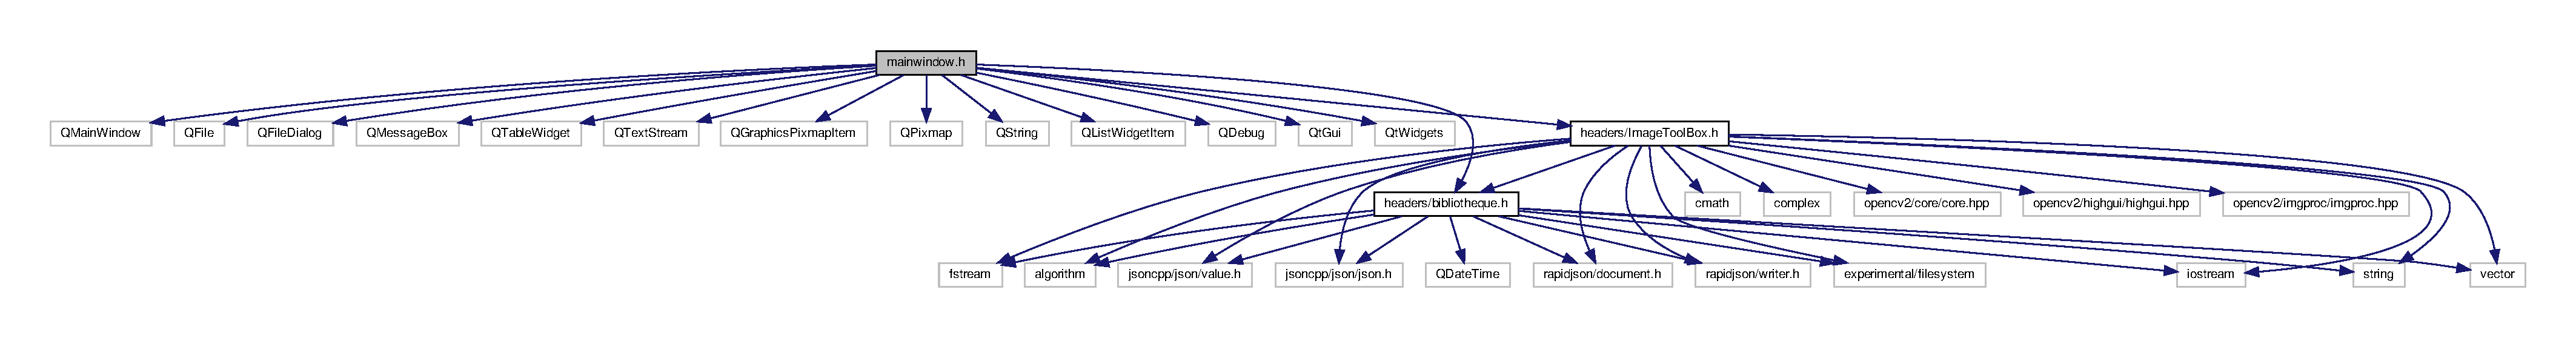
\includegraphics[width=350pt]{mainwindow_8h__incl}
\end{center}
\end{figure}
\subsection*{Classes}
\begin{DoxyCompactItemize}
\item 
class \hyperlink{classMainWindow}{Main\+Window}
\begin{DoxyCompactList}\small\item\em The \hyperlink{classMainWindow}{Main\+Window} class. \end{DoxyCompactList}\end{DoxyCompactItemize}


\subsection{Description détaillée}
Header de la classe \hyperlink{classMainWindow}{Main\+Window} de QT. 

\begin{DoxyVersion}{Version}
0.\+1 
\end{DoxyVersion}
\begin{DoxyDate}{Date}
2022-\/01-\/22
\end{DoxyDate}
\begin{DoxyCopyright}{Copyright}
Copyright (c) 2022 
\end{DoxyCopyright}

%--- End generated contents ---

% Index
\backmatter
\newpage
\phantomsection
\clearemptydoublepage
\addcontentsline{toc}{chapter}{Index}
\printindex

\end{document}
